\documentclass[11pt]{report}

%% Language and font encodings
\usepackage[english]{babel}
\usepackage[utf8x]{inputenc}
\usepackage[T1]{fontenc}
\usepackage{graphicx}
\usepackage{amsfonts}
\usepackage{dsfont}
\usepackage{bm}
\graphicspath{ {images/} }
%% Sets page size and margins
\usepackage[a4paper,top=3cm,bottom=2cm,left=3cm,right=3cm,marginparwidth=1.75cm]{geometry}

%% Useful packages
\usepackage{amsmath}
\usepackage[colorinlistoftodos]{todonotes}
\usepackage[colorlinks=true, allcolors=blue]{hyperref}
\usepackage{braket} % needed for \Set
\usepackage{caption}
\usepackage{algorithm}
\usepackage[noend]{algpseudocode}
\usepackage{float}
\usepackage{subcaption}
\usepackage{appendix}
\linespread{1.3}

%%declarations
\usepackage{xspace}                                                             
\DeclareRobustCommand{\eg}{e.g.,\@\xspace}                                      
\DeclareRobustCommand{\ie}{i.e.,\@\xspace}                                      
\DeclareRobustCommand{\wrt}{w.r.t.\@\xspace}                                    
\DeclareRobustCommand{\wp}{w.p.\@\xspace}
\DeclareRobustCommand{\quotes}[1]{``#1''}
\usepackage{dsfont}
\usepackage{bm}
\newcommand{\mathbr}[1]{\bm{\mathbf{#1}}}

\usepackage{amsthm}

\DeclareMathOperator*{\argmax}{arg\,max}
\DeclareMathOperator*{\argmin}{arg\,min}
\newtheorem{definition}{Definition}[section]
\newtheorem{theorem}{Theorem}[section]
\newtheorem{prop}{Proposition}[section]
\newtheorem{ass}{Assumption}[section]
\newtheorem{coroll}{Corollary}[section]
\newtheorem{lemma}{Lemma}[section]
\newtheorem{example}{Example}[section]

\usepackage[english]{babel}
\renewcommand{\captionfont}{\small}
\newcommand{\ev}{\displaystyle \mathop{\mathbb{E}}}
\newcommand{\Var}{\displaystyle \mathop{\mathbb{V}\mathrm{ar}}}
\newcommand{\Cov}{\displaystyle \mathop{\mathbb{C}\mathrm{ov}}}
\newcommand{\Bias}{\displaystyle \mathop{\mathbb{B}\mathrm{ias}}}

\pagenumbering{roman}
\begin{document}
\title{
	Driving Exploration Through Particle Q-Distributions
}
\thispagestyle{empty}
\begin{titlepage}
\vspace*{-1.5cm} \bfseries{
\begin{center}
  \Large
  POLITECNICO DI MILANO\\
  \vspace*{0.3cm}
  \large
  \textsc{School of Industrial and Information Engineering}\\
  \normalsize
  Department of Electronics, Information and Bioengineering\\
  Master of Science Degree in Computer Science and Engineering\\
  \vspace*{0.8cm}
  \begin{figure}[htbp]
    \begin{center}
      
\includegraphics[width=4cm]{Logo-pol.jpg}
    \end{center}
  \end{figure}
  \vspace*{0.3cm} \huge



  \textbf{Driving Exploration Through \\ Particle Q-Distributions}\\


  \vspace*{.75truecm} \large
  AI \& R Lab \\
  The Artificial Intelligence and Robotics Lab\\
  of the Politecnico di Milano
\end{center}
\vspace*{3.0cm} \large
\begin{flushleft}


  Supervisor: Prof. Marcello Restelli \\
  Co-supervisor: Dott. Alberto Maria Metelli
  
  \end{flushleft}
\vspace*{1.0cm}
\begin{flushright}


  Author:\\ Amarildo Likmeta, 872023 \\ 


\end{flushright}
\vspace*{0.5cm}
\begin{center}



  Academic Year 2017-2018
\end{center} \clearpage
}
\end{titlepage}

\chapter*{Abstract}
\par
The various sequential decision making problems are one object of study of Artificial Intelligence. Reinforcement learning addresses these problems in a trial and error way.  An agent is required to interact with an environment and collect experience from these interactions which in turn are used to find the optimal policy to pursue. One core element of reinforcement learning is the reward signal that the agent receives from the environment telling the agent if some states are desired or they should be avoided. This reward is assumed to be immediate after each action and the goal of the agent is to maximize the cumulative reward collected during its activity in the environment. Defined in this way, the reward function specifies the task to be learned by the agent.\par
The Exploitation- Exploration trade-off remains a main topic in reinforcement learning. The problem consists in balancing reward maximization using the knowledge acquired at the moment with exploring new actions to improve the knowledge of the environment. Traditionally exploration has been explicitly added to algorithms by occasionally choosing actions randomly instead of relying on the experience collected, nonetheless it remains a major challenge in reinforcement learning. Common exploration strategies, such as $\epsilon$-greedy, fail to conduct temporally-extended or deep exploration. This not only causes exponentially larger data requirements for the algorithms, but most importantly might cause premature convergence of the algorithms to a suboptimal policy or might prevent convergence altogether.\par
Traditionally reinforcement learning faces these problems by estimating the value function  which estimates how ``good'' the states are (or action-states pairs in the case of action-value function). Being that the agents interact with an ``uncertain'' environment the value-function is the expected cumulative reward collected in the long term. In this thesis we build on recent work advocating the use of Q-distributions to drive exploration. By explicitly modeling the distribution of the Q-values instead of just estimating the mean we are able to make more informed decisions and use these distributions to drive exploration. Starting from a prior distribution we can update our knowledge with each new sample using a Bayesian approach and we can also use these distributions to quantify the Exploration-Exploitation trade-off.\par
We start by introducing our new approach in simple finite domains, designed to emphasize exploration, for later extending it to continuous domains.   We compare our approach with state of the art algorithms in Taxi , Loop, Chain, SixArms, RiverSwim and KnightQuest domains as well as in various Atari games from the Arcade Learning Environment.

\chapter*{Acknowledgements}
I would like to thank Prof. Marcello Restelli, supervisor, and Dott. Alberto Maria Metelli, co-supervisor for the constant support and guidance in writing this thesis. They were a constant source of inspiration and my first contact with the research world. I would like to also thank Dott. Carlo D'Eramo for support in implementing some of the algorithms discussed in this thesis.\par 
Moreover, I would like to thank all my friends for supporting me and specially for putting up with me during the time I worked in this thesis. A special thanks goes to the residents and managers of the "La Presentazione" student residence in Como, where I did most of the work discussed in this thesis.\par
The most important thanks goes to my family. They have always been there for me, always supporting and pushing me to achieve my dreams. This thesis is dedicated to them.
\begin{flushright}


  Amarildo \\ 04 10 2018 \\ 


\end{flushright}

\tableofcontents

\listoffigures

\listofalgorithms

\chapter{Introduction}
\pagenumbering{arabic}
Technology is continuously growing in terms of complexity and capabilities, whereas society is evolving and increasingly relying on computers to make decisions and to take actions on its behalf. Next-generation computer systems, too complex to manage for humans , will need to configure, optimize, and repair themselves. Self-driving cars are already on our roads, relieving humans of the monotony of driving during rush hours. Robots will accept tasks that are too dangerous for humans, from fighting fires to exploring disaster areas. These are just a few examples of \emph{autonomous agents} taking actions without human intervention to achieve some task. A key research question is how to make these agents’ behaviors robust like human decision-making. \par
Determining fixed behaviors in advance yields agents that fail to adapt to the inevitable unforeseen situations and uncertainty that characterize real-world tasks. To replicate human expertise, agents must replicate the human ability to learn and adapt. These \emph{learning} agents choose future behaviors in response to past behavior data. The learning agent needs to account for the delayed effect of its
decisions, along with the possible non-determinism of the environment. Clearly, in
order to plan a good decision, the agent must refer to some notion of \emph{optimality}. In real-life, optimality is not necessarily expressed in a formal way, however, when
a sequential decision-making problem is tackled from the point of view of Artificial
Intelligence (AI) we need to specify some notion of \emph{goal}. A \emph{goal-directed agent} is able not only to react to the changes of the environment, but also to show a proactive behavior, intended to achieve its goal. Differently from classic optimal control, no assumption is made on the knowledge of the dynamics of the environment, so the controller cannot be designed a priori, but needs to be learned from the interaction with the environment.\par
We will consider those problems that satisfy the Markov property, \ie the next state of the environment does not depend on the past states and actions given the current state and action, as well as the decision of the agent is determined as a function of the current environment state only. This requirement, while apparently unrealistic, can always be assumed provided that the representation of the environment state is
sufficiently rich (e.g., we can define a rich state as the concatenation of all the states and actions visited so far; in this way we embed the whole history in a single state). Such problems can be cast into the Markov Decision Processes (MDP) framework. The goal of learning agents in this environment is usually to maximize some sort of  \emph{utility function}. Whenever the agent performs an action, it receives a feedback from the environment, the \emph{immediate reward}, which depends, in the most general case, on the starting state, the action performed and the landing state. The utility, from a given state, is defined as the \emph{cumulative reward}, \ie the sum (possibly discounted) of the rewards collected along the visited states.\par
Reinforcement learning (RL) provides an appealing framework for developing learning agents. It grew out of promising early algorithms ~\cite{Watkins:89,rummery:cuedtr94} that guarantee convergence to optimal behavior in arbitrary finite agent-environment systems. These algorithms achieve these theoretical guarantees by estimating the long-term value of every state in the system. However, convergence to the correct values requires an infinite amount of data from each state (asymptotic convergence) and, in practice, these methods are rarely feasible in realistic applications. RL research has focused on scaling these methods on harder problems, working towards the goal of a relatively simple learning algorithm that allows an agent to cope with the complexity of the real world.\par
Interesting problems, especially tasks that are easy solvable by humans, suffer from the \emph{curse of dimensionality} in the sense that the state space size is usually exponential in the number of dimensions. It is thus not possible to brute force all the possible combinations of actions and save the best. There is an increasing need for smart strategies on how to explore the environment and decide when the agent should explore.
The natural counterpart of exploration is exploitation.  Both together form one of the fundamental challenges in RL: the Exploration vs. Exploitation dilemma~\cite{Sutton:1998:IRL:551283}. If some knowledge is obtained about the environment, the agent should use it to receive higher rewards. Logically pure random exploration is not enough to get high rewards. Therefore, imagine a human who has recently moved to a new city. During the first week he/she explores the city center by taking some randomly chosen routes through it. With this technique, he/she is going to find some spots, which match his/her personal interests. However if he/she decides to visit the best places, he/she found during the first week he/she might lose the opportunity to find other places, which are even better, because he/she stopped exploring the environment.\par
In order to solve the exploration vs. exploitation problem several strategies have been proposed. There are very simple ones, e.g., $\epsilon$-greedy strategies, used extensively in the literature in classic approaches ~\cite{Watkins:89,rummery:cuedtr94} as well as modern ones ~\cite{mnih2015humanlevel,DBLP:journals/corr/OsbandBPR16}. The drawback of these simple strategies is that they tend to need exponential many examples of states and actions and thus suffer from the curse of dimensionality as well. For example, take the Deep Q Network (DQN) architecture that was the first capable of playing Atari games at a human level ~\cite{mnih2015humanlevel}. Its actions are based solely on raw input pixel data, one of the main steps in designing a generally closed perception system.~\cite{mnih2015humanlevel} and perfomed on various Atari 2600 games well. However, a prominent example in which DQN fails is Montezuma’s Revenge. In this game, the player has to find several keys to unlock the doors unveiling the way to higher levels. The main reason for the malfunction is insufficient exploration in the regions of sparse rewards.\par
More advanced methods for exploration have been proposed in the literature. Some of them fall into the category of \emph{model-based} algorithms ~\cite{Kearns:2002:NRL:599616.599699,Brafman:2003:RGP:944919.944928,NIPS2006_3052}. They estimate the parameters of the underlying MPD model and use uncertainty about these estimates to drive exploration. \emph{Model-free} algorithms that perform efficient exploration have also been proposed ~\cite{Strehl:2006:PMR:1143844.1143955,Dearden98bayesianq-learning}. Some of these algorithms offer theoretical guarantees on the number of transitions they need to learn the optimal policies ~\cite{Kearns:2002:NRL:599616.599699,Brafman:2003:RGP:944919.944928,NIPS2006_3052,Strehl:2006:PMR:1143844.1143955}, but these theoretical bounds are either too lose, or apply only to small finite problems or both. Recent methods have been proposed to scale efficient and deep exploration in large problems, where function approximation (e.g., \emph{deep networks}) is used to generalize over the large state space ~\cite{DBLP:journals/corr/OsbandBPR16}. More recently, \emph{distributional reinforcement learning}, although it is not developed mainly to address the exploration problem, has been used to drive deep exploration in the context of \emph{deep reinforcement learning} ~\cite{DBLP:journals/corr/BellemareDM17,DBLP:journals/corr/abs-1710-10044}.
\par
This thesis continues in the tradition of scaling RL algorithms to harder tasks. We focus on the classical problem of balancing what is referred to as \emph{exploitation}: the estimation of optimal behavior given the existing data, with \emph{exploration}: the generation of behaviors intended to gather data that will improve future attempts at exploitation. In particular, most RL algorithms estimate optimal behavior from existing data while assuming that new data will not become available. They then modify this behavior to encourage the acquisition of new data, in the simplest case just by adding random actions. We advocate the development of agents, that explicitly  consider the uncertainty of their knowledge about the environment so that they can choose future behaviors in order to improve the usefulness of future data. By gathering more data, the agent improves its future ability to exploit the environment. This approach draws inspiration from human learning, which is most effective in the context of active experimentation, not passive observation. 
\subsubsection{Goal}
The goal of this thesis is to develop a model-free Reinforcement Learning algorithm that is able to perform efficient and deep exploration by explicitly representing the uncertainty  about its current Q-value estimates. 
\section{Overview}
The contents of this thesis are organized in the following five chapters. We start
in Chapter ~\ref{chap:chapter2} with an overview of the different aspects of Markov decision processes and reinforcement learning. We introduce definitions and discuss several aspects, such as value functions and optimal policies. Moreover, we outline the techniques for solving MDPs, starting with dynamic programming and presenting the most popular reinforcement learning approaches, along with  a brief discussion to function approximation methods. Finally, we give an overview of distributional reinforcement learning. The focus of the presentation is directed to the aspects that will be exploited in the subsequent chapters. Furthermore, in this chapter,
we introduce the notation that we will use throughout the thesis.\par
In Chapter ~\ref{chap:chapter3} we depict the landscape of the state-of-the-art algorithms in efficient exploration. The algorithms are presented in overlapping categories that group together methods that share similarities in the approach. For each category we mainly address a representative algorithm discussed in detail, emphasizing pros and cons. The goal of this chapter is to guide the reader in a conscious understanding of the fundamental motivations of this work.
Chapter ~\ref{chap:chapter4} is devoted to the extensive description of Particle Q-Learning. We begin by discussing our representation of the uncertainty of the agent using Q-distributions and present our main results about the approximation of the Q-distribution using a \emph{mixture of deltas} and how to update the distributions with new samples. Then we illustrate two policies that use the Q-distributions to make more informed decisions to balance exploration and exploitation. Finally, we discuss how to maintain our Q-distributions online, by using samples of the \emph{local immediate reward}.\par
In Chapter ~\ref{chap:chapter5} we evaluate Particle QL against popular RL methods. We first introduce the metrics we use to compare the performance of the algorithms. Then, for the considered domains, we analyze the performance in terms of \emph{learning speed} and we show how the Q-distributions shrink and how the uncertainty about the Q-values goes to 0. Besides the experiments in small domains, designed to require exploration, we evaluate our algorithm in the Atari suite of games, comparing our results with Bootstrapped DQN ~\cite{DBLP:journals/corr/OsbandBPR16} a recent deep RL algorithm that performs deep exploration. We test the algorithms in various Atari games, including the infamous Montezuma's Revenge.\par
In Chapter ~\ref{chap:chapter6} we summarize the most relevant achievements of this thesis and we highlight the strengths and weaknesses of the proposed approach. Furthermore, we suggest possible extensions of this work.

\chapter{Reinforcement Learning and Markov Decision Processes} \label{chap:chapter2}
Reinforcement Learning (RL) is an area of machine learning, closely tied to behavioral psychology, concerned with how agents should behave in their environment as to maximize some notion of utility function. Being inspired from psychology, we can say that this area is the closer to how humans and other beings learn.  The agent has to explore  environment, collecting data on its interactions and using them to make informed decisions in the future. In a way this process is similar to a baby exploring his surroundings and playing in a playground. The process is formalized in Figure \ref{fig:rl_framework}.\par
\begin{figure}
  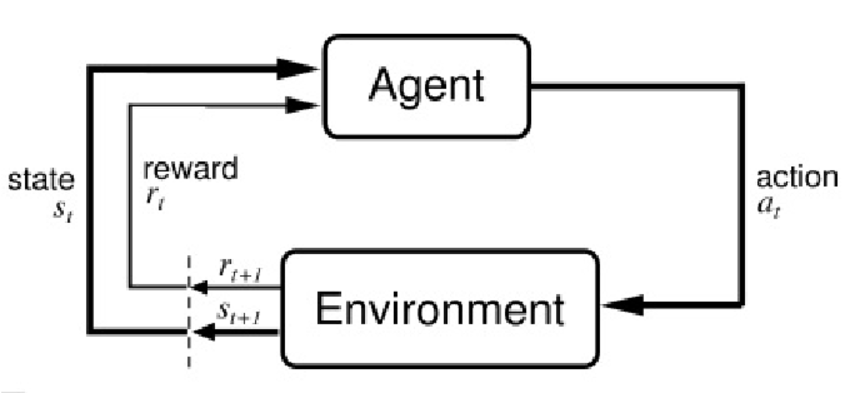
\includegraphics[width=\linewidth]{RL.png}
  \caption{The Reinforcement Learning framework ~\cite{Sutton:1998:IRL:551283}}
  \label{fig:rl_framework}
\end{figure}
The main driver of the agent's behavior is the reward signal it receives from the environment.  In the baby's case, the activity of exploring the playground and playing, is driven by an intrinsic motivation of human beings to explore our surroundings and understand them better, which in this case can be seen as an internal, or intrinsic reward signal. Other examples include teaching rats how to solve a maze by giving them food if they reach the end. In this case the reward signal is external or extrinsic. In either case the reward function  specifies the task the agent has to learn. We assume that the reward is given to the agent after every action but in the most interesting and complicated cases actions might affect not only the immediate rewards but also future rewards. So the agent must have the ability to map the sensations it gets from the environment (states) to actions, keeping in mind the effects of these actions in the future. This kind of problems are best described in the Markov Decision Process (MDP) framework.\par
Reinforcement Learning is fundamentally different from supervised learning. In the latter, learning is conducted on a training set of labeled samples provided by an external knowledgeable source (supervised)~\cite{hastie_09_elements-of.statistical-learning}. Each sample is a representation of the situation together with specification of the correct behavior of the system in this situation. This kind of learning is used to generalize from this training dataset, and apply a correct behavior in future situations not present in the train set. Even though it is a really important part of machine learning, supervised learning alone is not enough to deal with control problems. In interactive problems it is often impractical to collect these datasets of the desired behavior, and even if this data is available it might be unreliable so the agents must be able to learn from their own experience. \par
Nonetheless supervised learning is often used together with reinforcement learning to tackle control problems. A famous example is the original AlphaGo~\cite{Silver_2016}, the first computer program able to beat an expert player in the ancient Chinese game of Go. The program was first trained to mimic the moves of expert players by using a database of historical moves containing more than 30 million moves. After it reached a certain level of mastery, using reinforcement learning methods,  the program was trained from experience by playing against other instances of itself. Even though this was a milestone in Artificial Intelligence, it was surpassed by the latest version of the program, Alpha Go Zero~\cite{silver2017mastering} , which skipped the initial supervised learning and learned to play the game totally by scratch and was able to beat the original game, 100 times in 100 games, showing the importance of reinforcement learning in control problems.\par
Reinforcement learning is also different from unsupervised learning which in literature is typically refereed as the area of machine learning concerned with finding structure hidden in large sets of unlabeled data~\cite{hastie_09_elements-of.statistical-learning}. Even though both rely on learning from unlabeled data, reinforcement learning is concerned with maximizing a reward signal received from the environment rather than discovering hidden features of the environment. Discovering features of the environment might be useful to reach the goal, but alone it is not enough to maximize the reward. For this reason, reinforcement learning is considered as a third machine learning paradigm~\cite{Sutton:1998:IRL:551283}.\par
Another aspect that distinguishes reinforcement learning form other paradigms of machine learning is the exploration vs exploitation dilemma, which is one of the greatest (if not the greatest) challenges of reinforcement learning and it does not arise in the other machine learning paradigms. Agents must be able  to apply the “best” actions in each situation  they face. To evaluate the value of each action they use the knowledge acquired from the interaction with the environment and to discover the best actions they need to explore the environment by applying new actions. So neither exploration or exploitation can be used exclusively to reach the goal of maximizing the reward. How do you balance the two? This dilemma is even more important in stochastic tasks, where actions have to be tried multiple times before having a reliable estimate of their value. This problem has been studied extensively for decades but no definitive solution has been found so far.\par
In this thesis, to address the exploration vs exploitation dilemma, we will turn to a distributional approach to Reinforcement Learning. The common approach to reinforcement learning models the expected cumulative reward received from each action in given states. By explicitly modeling the distribution of the return estimate, instead of the expected value we are able to have a better estimate of the value of each action and to quantify the exploration dilemma, thus making better decisions.~\cite{Dearden98bayesianq-learning}\par
This chapter is meant to introduce main concepts of reinforcement learning used in further chapters. The chapter is organized as follows. We start in Section ~\ref{MDPs} where we introduce the concept of Markov decision process, the notion of value function and we formalize the optimality criteria. Section ~\ref{planning_mdps} briefly presents the notion of planning in MDPs and  dynamic programming, the standard approach to solve MDPs, when the model of the environment is available. Section ~\ref{reinforcement_learning} gives a classification of RL algorithms and describes the most important model-free algorithms. In Section ~\ref{sec:function_approximation} we shortly discuss function approximation. Finally, Section ~\ref{distributional_rl_section} is devoted to distributional RL and the fundamental importance of the value distribution.
\section{Markov Decision Processes} \label{MDPs}
Markov Decision Processes (MDPs) provide a mathematical framework for modeling sequential  decision making problems in situations where the outcomes are partly random and partly in control of a goal-directed agent, which interacts with an environment by performing actions and sensing perceptions. In this thesis we consider discrete time  MDPs, in which the agent has to decide which action to take in each state so that he maximizes his utility function. At each time step the agent perceives a state  from the environment, and after choosing an action he perceives the next state he moved to and a reward signal associated with this transition, called  immediate reward. Usually the utility function of the agent is some sort of cumulative reward calculated on an extended time frame. Maximizing the immediate rewards might not be enough to maximize the cumulative reward so many times the agent has to sacrifice immediate rewards to gain in the long  term.\par
Markov Decision Processes are an extension of Markov Chains. The difference is the addition of actions (allowing choice of the agent) and rewards (providing motivation to the agent). So if we have only one action , and all the rewards are the same  an MDP reduces to a Markov Chain. These processes are called Markov, because they have what is known as the Markov property, that is, that given the current state and action, the next  state is independent of all the previous states and actions. The current state captures all that is relevant about the world in order to predict what the next state will be.   
\subsection{Definitions}
Different definitions are available in literature. We consider the following one:
\begin{definition}
	A Markov Decision Process is a \emph{tuple} $\mathcal{M= (S, A, P, R, \mu, \gamma)}$ ,
where:
\end{definition}
\begin{itemize}
\item $\mathcal{S}$ is a \emph{non-empty measurable} set , called \emph{state space};
\item $\mathcal{A}$ is a \emph{non-empty measurable} set , called \emph{action space};
\item $\mathcal{P}$ is a function $\mathcal{P: S\times A\rightarrow}\Delta \mathcal{S}$ called \emph{transition model}, that for all  $s \mathcal{ \in S}$ and for all  $a\mathcal{\in A}$, assigns $\mathcal{P}(\cdot\mid s,a)$, a probability measure over $\mathcal{S}$,$P(\cdot\mid s,a)$ being the corresponding probability density function;
\item $\mathcal{R}$ is a function $\mathcal{R: S\times A \times S\rightarrow \Delta \mathbb{R}}$ called \emph{the reward function}, that for all  $s,s' \mathcal{ \in S}$ and for all  $a\mathcal{\in A}$, assigns $\mathcal{R}(\cdot\mid s,a,s')$, a probability measure over $\mathbb{R}$,R$(\cdot\mid s,a,s')$ being the corresponding probability density function and R(s,a)= $\mathbb{E}_{\substack{\text{$ s'\sim P(\cdot\mid s,a)$} \\ \text{$r \sim R(\cdot\mid s,a,s')$}}} [r] $ is the state-action expected reward;
\item $\mu$ is a probability measure over $\mathcal{S}$ called distribution of the initial states, $\mu(\cdot)$ being the probability density function;
\item $\gamma \in [0,1]$ is the \emph{discount factor}. 
\end{itemize} \par
The state space $\mathcal{S}$ and the action space $\mathcal{A}$ define the sensor and actuator possibilities of the agent. They can be either finite or infinite, discrete or continuous. Sometimes not all the actions are performable in all states, in this case it is convenient to define the set $\mathcal{A}(s)$ for all $s\mathcal{ \in S}$ which is the set of actions available in state s, therefore $\mathcal{A}= \bigcup_{s∈S}A(s)$\par
The immediate payoff is modeled by means of a scalar reward, that given the current state $s$, the current action $a$ and the next state $s′$ assigns for all Borel sets $A \in B(\mathbb{R})$ the quantity $R(A|s, a, s′)$ that is the probability to get a payoff in $A$ by starting from state $s$, performing action $a$ and ending up in state $s′$. $R(\cdot|s, a, s′)$ is the corresponding density function. In most common applications the state-action expected reward $R(s, a)$ is used,  defined as the expected value of the reward taken over all next states $s′$ and all real rewards $r$. Sometimes it is convenient to consider the state-action-state expected reward $R(s, a, s′) = \mathbb{E}_{r∼R(\cdot|s,a,s′)} [r]$. We will also assume that the immediate reward is upper bounded in absolute value, \ie $\parallel R\parallel_{\infty} = \max_{s\in \mathcal{S}} \max_{a \in \mathcal{A}} \mid R(s,a)\mid \leq M < +\infty $.\par
The reward function ultimately defines the goal of the agent in its environment. Is a scalar reward enough to specify every goal? Sutton and Burto~\cite{Sutton:1998:IRL:551283} hypothesize that all that we call \emph{goal} can be expressed as maximizing the cumulative sum of a received scalar reward signal. Although not proven, this hypothesis is so simple and powerful that we need to disprove it before looking for something more complicated.\par
The time is modeled as a discrete set of time steps, typically represented as a sequence of natural numbers $\mathcal{T} = {0, 1, \ldots, T }$ where $T$ is called \emph{horizon} and can be either finite $T \in \mathbb{N}$ or infinite $T = \infty$. In the former case the MDP is said to be \emph{finite horizon}, otherwise it is called \emph{infinite horizon}. An MDP is said episodic if the state space contains a \emph{terminal} (or absorbing) state, \ie a state $s$ from which no other states can be reached (for all actions $a \in \mathcal{A}, P(s|s,a)= 1$). Typically, it is assumed that all actions performed in a terminal state yield zero reward.\par
The discount factor $\gamma$, which is typically strictly less than 1, causes rewards perceived further in time to be weighted less. This is especially important in infinite horizon MDPs, but might be useful also in finite horizon cases. A typical example where applying a discount factor less than 1 are financial applications where receiving monetary rewards in the present usually is more valuable than receiving them in the future due to the interest rate.\par
To recap, the dynamics of MDPs are as follows. We start from an initial state $s_{0}$ drawn from the initial state distribution $\mu$. At each time step the agent choses an action from the available set of actions $A(s)$. Following the transition model $P(\cdot \mid s,a)$ it ends in state $s'$ and it observes the reward signal $r$ drawn from the reward model $R(\cdot \mid s,a,s')$. By repeatedly applying these activity the agent traverses a sequence of states collecting a sequence of rewards. Maximizing the ($\gamma$ discounted) cumulative sum of these rewards is the agents goal.
\subsection{Policies}
As we said before the goal of an agent is to maximize some sort of cumulative reward by taking actions that produce larger rewards. Generally the agent uses the history of states he has traversed ($s_0, s_1...$) to make decision on future actions as to maximize his utility function. The set of rules mapping the agents history to actions are called \emph{policies}. But because MDPs have the Markovian property, the current state ,$s_t$ is enough to determine the next action $a_t$~\cite{Sutton:1998:IRL:551283}. These kind of policies are called, not surprisingly, Markovian Policies. Moreover if the actions mapped are not dependent on the time step $t$, the policy is called stationary. In this thesis,for simplicity, when we use the term policy we will refer to Markovian Stationary Policies. More formally:
\begin{definition}
	A Markovian Stationary Policy $\pi$ is a function $\pi:\mathcal{S}\rightarrow \Delta(A)$ that for every state $s \in \mathcal{S}$ maps a probability distribution, $\pi(\cdot \mid s)$, over the action space $\mathcal{A}$. If the policy is deterministic then $\pi:\mathcal{S}\rightarrow A$
\end{definition}
The goal of reinforcement learning becomes finding the policy that maximizes the cumulative reward collected.
An MDP paired with a policy $\pi$ induces what in literature is called a \emph{Markov Reward Process} denoted by the tuple $\mathcal{(S,P^\pi,R^\pi,\gamma,\mu)}$. For all states $s \in \mathcal{S}$, $\mathcal{P^\pi}(\cdot \mid s)$ is a probability measure over $\mathcal{S}$. $P^\pi$ is the probability density function obtained by marginalizing the transition model of the MDP, $\mathcal{P}$ over the actions:
\begin{equation}
	P^\pi(s'|s)=\sum_{a \in \mathcal{A}} \pi(a|s)P(s'|s,a) \qquad \forall s,s' \in \mathcal{S}
\end{equation}
$P^\pi(s'|s)$ gives the probability of ending up in state s', starting from state s, in one time step. Similarly,$\mathcal{R^\pi}(\cdot|s,s′)$ for all $s,s′\in \mathcal{S}$ is a probability measure over $\mathbb{R}$ with the corresponding density function $R$ obtained from the reward model of the MDP as:
\begin{equation}
	R^\pi(r|s,s')=\sum_{a \in \mathcal{A}} \pi(a|s)\mathcal{R}(r|s,s',a) \qquad \forall s,s' \in \mathcal{S}
\end{equation}
MRPs are a suitable model for uncontrolled processes. The notion of action disappears and they can be used to model stochastic processes taking place in the environment and producing rewards. By further removing the concept of reward from the MRPs, as mentioned before we are left with Markov Chains or Markov Processes.
\subsection{Utility Functions and Value Functions}
Given a policy $\pi$, played by an agent in an MDP, it is possible to define the utility of each state. While the reward signal measures the immediate payoff the agent experiences, the utility function of a state measures the reward in a long run. The utility function is calculated over trajectories, and measures how ``good'' that trajectory is to the agents. Typically the utility is a sum (possibly discounted) of the rewards collected during the trajectory , even though there are other types of utility functions defined in literature~\cite{Puterman:1994:MDP:528623}. \par
If $\tau$ is a trajectory the agent followed under policy $\pi$,starting form the initial state distribution $\mu$, the expected discounted sum of rewards is defined as:
\begin{equation}
		J^{\pi}=E_{\tau \sim p(\cdot |\mu,\pi,\mathcal{P})}\left[ \sum_{t=0}^{T(\tau)} R(s_{\tau,t},a_{\tau,t})\right]
\end{equation}
where :
\begin{itemize}
\item $T(\tau)$ is the length of trajectory $\tau$;
\item $s_{\tau,t}$ is the state where the agent is in the t-th time step of trajectory $\tau$;
\item $a_{\tau,t}$ is the action taken in the t-th time step of trajectory $\tau$.
\end{itemize}
To avoid the potential divergence of the utility function in the case of infinite MDP, a discount factor is introduced and the utility function becomes the discounted expected cumulative reward also known as \emph{expected return}~\cite{Sutton:1998:IRL:551283}.
\begin{equation}
		J^{\pi}=E_{\tau ~p(\cdot |\mu,\pi,\mathcal{P})}\left[ \sum_{t=0}^{T(\tau)} \gamma^{t}(s_{\tau,t},a_{\tau,t})\right].
\end{equation}
By introducing the discount factor we avoid the divergence of this measure, holding the assumption that the reward signal is upper bounded. The discount factor is open to multiple interpretations. From an economical/financial point of view the discount factor accounts for the fact that an agent might be more interested in a payoff obtained in the near future rather than a payoff obtained far in the future. Values of $\gamma$ close to 0 lead to a "miopic” evolution (at the limit in which $\gamma$ = 0 the agent is interested only in the immediate reward and the solution of the problem is obtained with a greedy policy) while values of $\gamma$ close to 1 lead to a “far-sighted” evolution.\par
From a statistical point of view the discount factor is related to the probability that the process continues for another epoch. If the MDP is episodic, \ie all trajectories reach an absorbing state, then $\gamma$ = 1 can be used. Formally, the discount factor is a parameter of the MDP. However, many times, $\gamma$ is tuned to favor the convergence of the RL algorithms. Small values of $\gamma$ improve the convergence rate. In the extreme case of $\gamma$ = 0 the problem degenerates in a greedy choice. However, small $\gamma$ could compromise the quality of the solution since the rewards collected in the far future become less important. Thus, the choice of $\gamma$, when possible, has to trade off
the quality of the recovered solution and the convergence speed of the algorithms.
\subsection*{Value Functions}
As we have already introduced, the goal of reinforcement learning is to find the optimal policy the agent can play to maximize his utility function. The most trivial way to do this is to list all the possible behaviors the agent can exhibit and chose the one with highest utility, using the utility functions mentioned above.Fortunately, we can do better than this.
A better way is to use the value function of each state, defined as :
\begin{definition}
The value function in state $s, V^\pi(s)$, of an MDP is the expected return starting from state $s$ and following policy $\pi$~\cite{Sutton:1998:IRL:551283}.
\begin{equation}
			V^\pi(s)=E_\pi \left[v_t| s_t=s \right] \qquad\qquad \forall s \in \mathcal{S},
\end{equation}
\end{definition}
where $v_t= \sum_{t=0}^{T(\tau)} \gamma^{t}(s_{\tau,t},a_{\tau,t})$. The problem of finding the optimal policy becomes finding the optimal value function, and determining the optimal behavior from it.\par
For control purposes, it is easier to compute the action-value function, $Q^\pi(s,a)$, as it is easier to determine the value of each action in each state, and then derive the optimal policy.The value function simply does not include enough information to determine the greedy action(the current best) for each state, at least without having the model of the MDP, where by model we refer to the state transition probabilities $\mathcal{P}$.
\begin{definition}
	The action-value function in state $s$ executing action a, $Q^{\pi}(s,a)$, of an MDP is the expected return starting from state $s$, applying action a and then following policy $\pi$ ~\cite{Sutton:1998:IRL:551283}
    \begin{equation}
			Q^\pi(s,a)=E_\pi \left[v_t| s_t=s,a_t=a \right] \qquad \qquad  \forall (s,a) \in \mathcal{S}\times \mathcal{A}.
	\end{equation}
\end{definition}
There is a clear relationship between the value function and the state value function. The former is computed by averaging the latter over the possible actions:
\begin{equation}
	V^\pi(s)=E_{a \sim \pi(\cdot|s)}\left[Q^\pi(s,a)\right] \qquad\qquad \forall s \in \mathcal{S}.
\end{equation}
Sometimes it is useful to estimate the \emph{advantage function}, $A^\pi(s,a)$ ~\cite{LeemonCBaird93}~\cite{SchulmanMLJA15}, which represents how much a given action, $a$, is convenient in state $s$, \wrt, the average utility of that state. $A^\pi(s,a)$ is defined as:
\begin{equation}
		A^\pi(s,a)=Q^\pi(s,a)-V^\pi(s) \qquad \qquad \forall (s,a)\in \mathcal{S} \times \mathcal{A}.
\end{equation}
\subsection{Bellman Equations and Operators}
We defined the state value function, $V^\pi(s)$, as the expected return collected stating from state $s$, and then following policy $\pi$. We can decompose this definition further by considering the value function as the sum of the immediate reward in state $s$ with the expected discounted reward in the following state. This kind of recursive definition will show itself useful in solving MDPs.

\subsubsection*{Bellman Expectation Equation}
The \emph{Bellman Expectation Equation}~\cite{Bellman:DynamicProgramming} is defined as :
\begin{equation}
\begin{split}
	V^\pi(s) & =E_\pi \left[ r_{t+1} + \gamma V^{\pi}(s_{t+1})|s_t=s \right] \\
    	& =\sum_{a\in A} \pi (a|s) \left( R(s,a)+ \gamma \sum_{s'\in S} P(s'|s,a) V^\pi(s')\right).
\end{split}	
\end{equation}
The action-value function can be decomposed in the same way as :
\begin{equation}
\begin{split}
	Q^\pi(s,a) & =E_\pi \left[ r_{t+1}+ \gamma Q^\pi(s_{t+1},a_{t+1})|s_t=s,a_t=a \right] \\
    	& =R(s,a)+ \gamma \sum_{s'\in S} P(s'|s,a) V^\pi(s') \\
        & = R(s,a)+ \gamma \sum_{s'\in S} P(s'|s,a) \sum_{a'\in A} \pi(a'|s') Q^\pi(s',a').
\end{split}	
\end{equation}
When the MDP is finite,by using the \emph{ Markov Reward Process} induced by policy $\pi$, we can write the Bellman Expectation Equation in a concise matrix form of the equation as follows:
\begin{equation}
	V^\pi=R^\pi+\gamma P^\pi V^\pi,
\end{equation}
which yields the solution:
\begin{equation}
	\label{eq:mdp_closed_form_solution}
	V^\pi=\left(I-\gamma P^\pi \right)^{-1} R^\pi.
\end{equation}
While this is an exact solution of the MDP , unfortunately inverting the matrix $\left(I-\gamma P^\pi \right)$ has a high computational complexity.\par
A way to solve the MDP while avoiding the complexity of the matrix inversion is to use the \emph{Bellman  Operator}~\cite{Bellman:DynamicProgramming} defined as $\mathcal{T}^\pi :\mathbb{R}^{(|S|)} \rightarrow \mathbb{R}^{(|S|)}$ :
\begin{equation}
(T^\pi V)(s)=\sum_{a \in A} \pi(a|s)\left(R(s,a)+ \gamma \sum_{s'\in S} P(s'|s,a) V(s')\right) \qquad \forall s \in \mathcal{S}/
\end{equation}

The Bellman Operator maps value functions to value function.It can be proved ~\cite{Puterman:1994:MDP:528623} that the state value function $V^\pi$ is the unique fixed point of the Bellman operator, $T^\pi$ , \ie it satisfies $T^\pi[V^\pi] = V^\pi $ (Bellman Expectation Equation).\par
We can define the Bellman Expectation Operator for the Q function as well ,$T^\pi : R^{S \times A} \rightarrow
R^{S \times A}$ , defined as:
\begin{equation}
(T^\pi Q^\pi)(s,a)=R(s,a)+ \gamma \sum_{s'\in S} P(s'|s,a) \sum_{a'\in A} \pi(a'|s') Q^\pi(s',a')  \qquad \forall (s,a) \in \mathcal{S} \times \mathcal{A}
\end{equation}
Like for the value function, $Q^\pi$ is the unique fixed point of $T^\pi$ , \ie $T^\pi[Q^\pi] = Q^\pi$.It is worth to notice that both operators are linear. Furthermore, they satisfy the contraction property in $\mathcal{L}_\infty$ norm, \ie $ \| T^\pi f_1 − T^\pi f_2 \| _{\infty} \leq \gamma \| f_1 − f_2 \| _{\infty}$ , thus the repeated application of $T^\pi$ makes any function converge to the value function.
Value functions are very important in reinforcement learning. They define a partial order over policies. Namely for any two policies $\pi, \pi'$:
\begin{equation*}
	\pi \geq \pi'\quad if \quad V^\pi(s) \geq V^{\pi'}(s) \qquad \forall s \in \mathcal{S}
\end{equation*}
\subsection{Optimality Conditions}
The standard approach to finding the \emph{optimal policy} of an MDP, \ie the policy that maximizes the agents utility function. is by means of the \emph{optimal value function}. The optimal value function maximizes the expected return for every state.\par
We will start by defining the optimal value function. If we call $\Pi$ the set of all possible Markovian policies then the optimal value function,$V^*$ is :
\begin{definition}
	Given an MDP $\mathcal{M}$, the optimal value function in any state $s \in S$ is given by :
\begin{equation}
	V^*(s)=\max_{\pi \in \Pi} V^\pi(s) \qquad \qquad \forall s \in \mathcal{S}
\end{equation}
\end{definition}
The optimal value function specifies the best possible performance an agent can reach in any state of the MDP. Solving an MDP means finding the optimal value function.Similarly we can define the optimal action-value function, $Q^*(s,a)$ as :
\begin{definition}
	Given an MDP $\mathcal{M}$, the optimal action-value function in any state-action pair $(s,a) \in S \times A$ is given by :
\begin{equation}
	Q^*(s,a)=\max_{\pi \in \Pi} Q^\pi(s,a) \qquad \qquad \forall (s,a) \in \mathcal{S} \times \mathcal{A}
\end{equation}
\end{definition}

\subsubsection{Bellman Optimality Equation}
Similarly with the value function of a given policy, we can define the optimal value function of an MDP in a recursive way ~\cite{Sutton:1998:IRL:551283}, as :
\begin{equation}
	\begin{split}
	V^*(s) &=\max_{a \in A}Q^*(s,a)\\
    &=\max_{a \in A}\left( R(s,a)+ \gamma \sum_{s' \in S} P(s'|s,a) V^*(s') \right)
	\end{split}
\end{equation}

\begin{definition}
The Bellman optimality operator, $T^*: \mathbb{R}^{|S|} \rightarrow \mathbb{R}^{|S|}$ is defined as:
\begin{equation}
	(T^*V)(s) =\max_{a \in A}\left( R(s,a)+ \gamma \sum_{s' \in S} P(s'|s,a) V(s') \right) \qquad \forall s \in \mathcal{S}.
	\label{eq:bellman_optimality}
\end{equation}
\end{definition}
As before a similar definition follows for the action-value
 optimality operator.This operator has the same properties as the Bellman Expectation Operator mentioned before, namely its a contraction \wrt $\|\cdot\|_\infty$, and the optimal value function $V^*$ is a unique fixed point of the operator.
 \subsubsection{Optimal Policies}
 Having defined the optimal value function and it is meaning, the question becomes is there any policy,$\pi^*$ whose corresponding value function coincides with the optimal value function? It can be shown~\cite{Sutton:1998:IRL:551283} that:
\begin{theorem}
For any Markov Decision Process 
\begin{itemize}
\item There exists an optimal policy $\pi^*$ that is better than or equal to all other policies $\pi \in \Pi$ 
\item All optimal policies achieve the optimal value function, $V^{\pi*}(s)=V^*(s)$
\item All optimal policies achieve the optimal action-value function, $Q^{\pi*}(s,a)=Q^*(s,a)$
\item There is always a deterministic optimal policy for any MDP
\end{itemize}
\end{theorem}
The last result is extremely important. As a result of the theorem above we can find the optimal policy of an MDP  by finding the optimal Q function, $Q^*$, and taking the  ``greedy'' action in each state.More formally :
\begin{equation}
			\pi^*(s)= \argmax_{a\in A}Q^*(s,a)	\qquad \qquad \forall s \in \mathcal{S}		
\end{equation}
It is worth noting that the knowledge of the optimal action value function $Q^*$ is sufficient to compute an optimal policy in a model-free manner,while the optimal value function $V^*$ requires the knowledge of the transition model $\mathcal{P}$. Model-free RL algorithms aim to estimate $Q^*$ from trajectories.
\section{Planning in MDPs} \label{planning_mdps}
We recall that an MDP is defined as the tuple $\mathcal{M}=(\mathcal{S,A,P,R},\mu,\gamma)$. If we know all the elements of the tuple we can solve the MDP (find the optimal policy) without ever taking an action in the environment~\cite{doi:10.2200/S00426ED1V01Y201206AIM017}. In AI, solving a decision making problem without ever making a decision is called \emph{planning}.Below we will describe some of the most used planning algorithms.
\subsection{Dynamic Programming}
Solving an MDP means finding an optimal policy. We are interested just in one policy, not the complete space of optimal policies. Having said this the usual approach is to find the optimal value function(or action-value function) and derive from it the optimal policy. When the state transition model of the MDP, $\mathcal{P}$, is known \emph{Dynamic Programming} is the most common approach used to solve MDPs. Dynamic programming ~\cite{Bellman:DynamicProgramming} is a common technique to solve problems that can be divided in subproblems.It is used to solve problems that satisfy two properties:
\begin{itemize}
\item Optimal Substructure \ie the solution can be decomposed into subproblems;
\item Overlapping subproblems \ie subproblems recur many times and solutions can be cached and reused.
\end{itemize}
When the subproblems are solved also the main problem is solved. This recursive thinking of problem might seem familiar as we described it before in the definition of the Bellman operator. In fact MDPs have both these properties.
\begin{itemize}
\item Bellman equation gives recursive decomposition;
\item Value function stores and reuses solutions.
\end{itemize}

\subsection{Policy Iteration}
Policy Iteration solves MDPs by alternating the \emph{policy evaluation} and \emph{policy improvement} phases~\cite{howard:dynamic60}.
\begin{figure}
  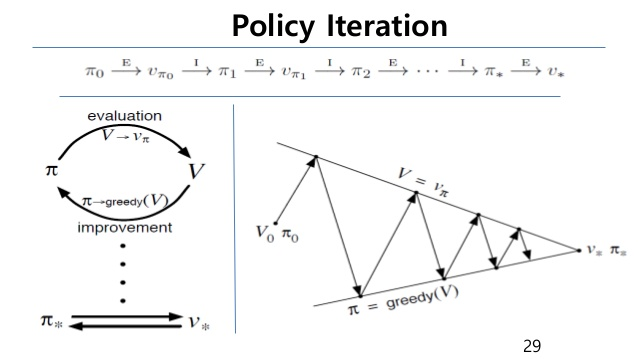
\includegraphics[width=\linewidth]{policy_iteration.jpg}
  \caption{Policy iteration algorithm (~\cite{Sutton:1998:IRL:551283}).}
  \label{fig:policy_iteration}
\end{figure}
The algorithm starts from a random policy, $\pi_0$, as shown in Figure ~\ref{fig:policy_iteration}. The policy iteration phase tried to extract the value function of the current policy. This can be done in various ways, mentioned in the previous section. The closed form solution could be used to get an exact solution(~\ref{eq:mdp_closed_form_solution}), but as we said before this comes with a high computational cost. Alternatively, we can apply recursively the Bellman Expectation Operator, which, as mentioned before, is a contraction in the max norm. By applying recursively this operator we get an approximation of the real value function of the policy, but for most applications look for an approximation of the value function. In fact in \emph{modified policy iteration}~\cite{Puterman:1978:MPI:2828482.2828486} the algorithm does not wait until convergence, advocating that a sufficiently good approximation is enough.\par
After the policy evaluation phase, policy improvement generates the greedy policy from the value function, by selecting, in each state, the action that maximizes it.
\begin{equation}
	\pi^{t+1}(s)=\argmax_{a \in \mathcal{A}} Q^{\pi^t}(s,a) \qquad \qquad s \in \mathcal{S}
\end{equation}
The policy generated is deterministic , and moreover it is guaranteed to be an improvement over the previous one.
\begin{theorem}
(Policy Improvement Theorem) Given an MDP $\mathcal{M}$ and two deterministic policies $\pi$ and $\pi′$ :
\begin{equation*}
	Q^\pi(s,\pi'(s)) \geq V^\pi(s) \qquad \forall s \in \mathcal{S} \qquad \Rightarrow \qquad V^{\pi'}(s) \geq V^\pi(s)	\qquad \forall s \in \mathcal{S}
\end{equation*}
\end{theorem}
Now, of course, by evaluating the policy by means of the value function, to generate the greedy policy, we need the state transition model, $\mathcal{P}$. In other cases, when the model is not available, Q-iteration is used. Here, instead of evaluating the value function of the policy, we evaluate the action-value function in a similar way.
\subsection{ Value Iteration}
Value iteration finds the optimal value function (and from it the optimal policy), without the intermediate use of policies. This method is based on the iterative application of the Bellman Optimality operation discussed in the previous section.\par
We recall that this operator is a contraction ~\cite{Banach1922}. The algorithm start from an initial (random) value function, $V^0$, and applies iteratively the Bellman operator until a stopping condition is met. The stopping condition might be maximal number of iterations or based on some minimal metric of distance between two subsequent estimations of the value function. In the end the optimal policy is recovered in the same way as in policy iteration, by taking the greedy policy induced by the optimal value function. Again the state transition model is required, otherwise we need to estimate the optimal action-value function instead.The convergence to the optimal value function is guaranteed. In particular, given two consecutive
approximations of the optimal value function we can bound the error \wrt the true optimal value function:
\begin{equation}
\|V^{t+1}-V^{s}\|_{\infty} < \epsilon \qquad \Rightarrow \qquad \|V^{t+1}-V^*\|_{\infty} < \frac{2 \epsilon \gamma}{1- \gamma}.
\end{equation} \par
While policy iteration represents explicitly the policy, value iteration focuses on the value function only. This means that intermediate value functions may not correspond to any policy. Both have polynomial time complexity for MDPs with fixed discount factor ~\cite{DBLP:journals/corr/abs-1301-6718}. Considering the single iteration, policy iteration is more computationally demanding \wrt, value iteration since it requires evaluating the policy and performing the greedy improvement, but it tends to converge in a smaller number of iterations. Besides DP, also Linear Programming (LP) can be employed to recover the optimal value function. However, LP becomes impractical at a much smaller number of states than DP methods do.
\section{Reinforcement Learning} \label{reinforcement_learning}
The main disadvantage of Dynamic Programming (when used to solve MDPs) is the fact that it requires the knowledge of the model. We need the state transition model to solve the MDP, which in real life problems is, more often than not, unavailable. Furthermore, DP becomes quickly infeasible as the action-state spaces of the MDP increase and it is clearly inapplicable for infinite MDPs. Reinforcement Learning tries to  convert DP algorithms in a sample-based nature. Sample based because we need to identify the underlying mechanisms of the environment since we do not have the transition model. 
\subsection{Classifying Reinforcement Learning Algorithms}
Reinforcement Learning, being one of the Machine Learning paradigms, is a vast field containing a large number of algorithms. We can classify RL algorithms in a number of ways as:
\begin{itemize}
\item Model-based vs Model-free depending whether or not the algorithm needs the state transition probabilities, $\mathcal{P}$. Model-free techniques try to find the optimal policy directly from samples of trajectories, whereas model-based techniques estimate first the transition model, to then apply DP to find the optimal policy
\item On-Policy vs Off-Policy depending on whether the agent learns the same policy used to collect data. On-policy algorithms learn the value function of the policy used to collect the samples, whereas off-policy algorithms learn the value function of a second policy (typically the optimal policy) while using a different policy to collect the samples.\
\item Online vs Offline depending on when the learning is performed. Online methods learn while collecting the samples whereas offline methods learn after they have all the data.
\item Tabular vs Function Approximation depending on the representation of the value function. Tabular methods explicitly save the value function for each state in a table (usable only in finite MDPs), whereas function approximation algorithms use approximators (regressors, neural networks) to estimate the value function.
\item Value-based vs Policy-based vs Actor Critic. Value-based algorithms estimate the value-function of the optimal policy (and from it the optimal policy). Policy-based algorithms try to estimate directly the optimal policy. Actor-critic methods have two parts. An actor(agent) that estimates the value function and a critic that updates it.
\end{itemize}
\subsection{Model-free Prediction}
The prediction problem aims to estimate the value function of a given policy.We will concentrate on the \emph{model-free} case, \ie when the transition model of the MDP is not known. We recall the process is now an MRP (MDP+ policy). The focus will be on two classes of algorithms, \emph{ Monte Carlo approches} (MC) and \emph{Temporal Difference approaches} (TD) ~\cite{Sutton:1998:IRL:551283}.Both methods are able to learn the value function of the policy directly from episodes of experience, whithout knowing the transition model of the MDP.They are able to do this by iteratively updating their estimation of the value function in each state.The updates are done using the exponential average update rule :
\begin{equation}
	V^{t+1}(s_t)=V^{t}(s_t)+ \alpha^t\left(v^{*}_t-V^{t}(s_t) \right),
\end{equation}
where $v^{*}_t$ is an estimation of the value function in state $s_t$ and $\alpha^t$ is the learning rate.\par
The two approaches differ on how the estimator $v^{*}_t$ is calculated. Monte Carlo learning:
\begin{itemize}
	\item Uses the simplest possible idea , value function is the sum of  (discounted) returns, $v^{MC}_{t}=\sum_{i=t}^{T(\tau)-1} \gamma^{t} r_{i+1}$;
	\item The approximator $v^{*}_t$ has the disadvantage the method is only usable for episodic MDPs. All episodes must terminate for the value function to be estimated;
	\item For the same reason can only be used for offline learning;
	\item States may be visited multiple times during an episode. When this happens we can either compute the value function just for the first visit of the state (first-visit MC) or for every time we visit the state (every-visit MC).The choice between the two boils down to the classical bias-variance trade off.~\cite{Sutton:1998:IRL:551283}.
\end{itemize}\par
TD on the other hand:
\begin{itemize}
	\item Leverages on bootstrapping to use the crrent approximation of the value function;
	\item The estimator is now the \emph{temporal difference target}, given by $v^{TD}_t=r_{t+1}+ \gamma V^{t}(s_{t+1})$;
	\item Bootstrapping allows for online learning and is not restricted to episodic MDPs;
	\item Bootstrapping after multiple timesteps gives rise to the $TD(\lambda)$ class of algorithms. We refer to ~\cite{Sutton:1998:IRL:551283} for more details.
\end{itemize}\par
Even though it can be shown that MC is an unbiased estimator ~\cite{Sutton:1998:IRL:551283} and TD is biased , in practice $TD(\lambda)$ is used more since it exploits the Markovian property of MDPs.
\subsection{Model-free Control}
The prediction problem deals with evaluating the value function a given policy. Whats more interesting about RL algorithms is the ability to learn a optimal policy in an MDP from samples of experience. This is called the \emph{model free control problem}. Control algorithms can be derived from the algorithms mentioned in the previous section by modifying them in a DP fashion. The main modification is estimating the Q function instead of the value function, since the model of the environment is not given. Second, and most importantly, we cannot apply the policy improvement step just by choosing the optimal action according to our current estimate. We are learning from samples, starting from an initial (possibly random) estimate.By choosing the optimal action, completely trusting our current estimate, we (almost surely) will converge to sub-optimal policies, since the samples we collect depend on our estimation of the Q function. This is in fact an instance of the \emph{exploitation vs exploration} problem. Do we use the information we have so far (exploitation) or we chose new actions to gather new informations (exploration) ? \par
An option is using an $\epsilon-greedy$ policy, a stochastic policy that chooses a random action, from the available ones, with probability $\epsilon$ and the current optimal action with probability  $1-\epsilon$. The $\epsilon-greedy$ Policy Improvement Theorem ~\cite{Sutton:1998:IRL:551283} shows that the new policy is an improvement \wrt, the previous one. As we collect samples, we become more confident about our estimate of the Q function and we can explore less. This can be done, in the simplest case, by defining a schedule for the \emph{exploration rate} $epsilon$, so that it converges to zero.We can now write the update rule for the Q function as :
\begin{equation}
	Q^{t+1}(s_t,a_t)=Q^{t}(s_t,a_t)+ \alpha^t\left(v^{*}_t-Q^{t}(s_t,a_t) \right).
\end{equation}
Again, different algorithms differ on their estimation of the value function, $v^{*}_t$.
MC uses the estimator $v^{MC}_{t}=\sum_{i=t}^{T(\tau)-1} \gamma^{t} r_{i+1}$, while TD as before uses $v^{TD}_t=r_{t+1}+ Q^{t}(s_{t+1},a_{t+1})$. The TD control algorithm is called SARSA ~\cite{rummery:cuedtr94}. The remarks made in the previous section about the usage of the two algorithms are valid also in the control setting. It is important to mention that both MC and TD are on-policy methods, meaning that they estimate the value function of a policy , while following it. This is important especially while bootstrapping in TD, since it determines the choice of the next action, $a_{t+1}$ that appears in the TD target. Both algorithms have convergence guarantees, as long as they follow the Robbin-Moore conditions on the learning rate, given by:
\begin{equation}
	\sum_{t=0}^{\infty} \alpha^{t}=+\infty \quad and \quad \sum_{t=0}^{\infty} \left(\alpha^{t}\right)^2 \leq +\infty.
\end{equation}
and  each state-action pair is visited infinitely many times ~\cite{Jaakkola:1994:CSI:1362288.1362296,Sutton:1998:IRL:551283}. A simple case that respects these conditions is $\alpha^t= \frac{1}{t}$.\par
We will now shortly present, an off-policy algorithm, used to estimate the optimal action-value function of an unknown MDP. The famous Q-Learning ~\cite{Watkins:89} can be thought as an extension of Value Iteration to the model-free case. Basically it applies a sample based version of the Bellman Optimality Equation, allowing to learn the optimal action value function without having to actually play an optimal policy The update rule of Q learning is given as:
\begin{equation}
	Q^{t+1}(s_t,a_t)= Q^{t}(s_t,a_t) +\alpha^t \left(r_{t+1} + \gamma \max_{a' \in \mathcal{A}} Q^{t}(s_{t+1},a') - Q^{t}(s_t,a_t)\right).
\end{equation}
Pseudocode of the Q learning algorithm is shown in Alg. [~\ref{alg:q-learning}].
\begin{algorithm}[H]
\begin{flushleft}
        \textbf{Input:} States $\mathcal{S} = \{1, \dots, n_s\}$, Actions $\mathcal{A} = \{1, \dots, n_a\}$, Reward function $R: \mathcal{S} \times \mathcal{A} \rightarrow \mathbb{R}$, Learning rate $\alpha \in [0, 1]$, Exploration rate $\epsilon \in [0, 1]$, Discount factor $\gamma \in [0, 1]$.\\
        \textbf{Input:} $Q$ function
\end{flushleft}
        \begin{algorithmic}
            \State Initialize $Q: \mathcal{S} \times \mathcal{A} \rightarrow \mathbb{R}$ arbitrarily
            \While{$Q$ is not converged}
                \State Start in state $s \in \mathcal{S}$
                \While{$s$ is not terminal}
                    
                    \State Chose $a$ according to Q and  $\epsilon-greedy $ exploration strategy 
                    \State Take $a$ and receive the reward $r$ and the new state $s'$
                    \State $Q(s', a) \gets (1 - \alpha) \cdot Q(s, a) + \alpha \cdot (r + \gamma \cdot \max_{a'} Q(s', a'))$
                    \State $s \gets s'$
                    \State Update learning rate $\alpha$ according to learning rate schedule
                    \State Update exploration rate $\epsilon$ according to exploration rate schedule
                \EndWhile
            \EndWhile
            \Return $Q$
        \end{algorithmic}
    \caption{$Q$-learning: Learn function $Q: \mathcal{S} \times \mathcal{A} \rightarrow \mathbb{R}$}
    \label{alg:q-learning}
\end{algorithm}
\section{Function Approximation} \label{sec:function_approximation}
Q-learning uses a tabular representation for the Q-function which is inapplicable when the state-action space is large, due to memory and time restrictions. Obviously, when the MDP is continuous a tabular representation is impossible. The solution proposed in literature is to estimate the value function with function approximation, i.e., $V^\pi(s) \approx \hat{V}(s)$. This approach tends to enforce generalization capabilities of the model and to speed up the computation \wrt tabular representation with no significant performance degradation when the approximators are carefully chosen.\par 
We can distinguish between parametric and non-parametric approximators: the former have a set of parameters known a priori, data are used to tune the values of the parameters (e.g., \emph{neural networks}); while for the latter the number of parameters is not fixed (e.g., \emph{decision trees}, \emph{nearest neighbors}).
\subsection{Basics of Function Approximation}
In the context of function approximation, learning can be defined as the process of
selecting a function $\hat{V}$ in a functional space $\mathcal{F}$ in order to minimize a loss function that encodes the fact that we aim to use $\hat{V}$ to approximate the value function $V^\pi$. We aim to solve the following problem:
\begin{equation}
\hat{V} = \argmin_{f \in \mathcal{F} } \Vert V^\pi - f \Vert_{q}.
\end{equation}
A fundamental issue at this point, is the \emph{bias-variance trade off}, closely related to the choice of the function space $\mathcal{F}$ ~\cite{hastie01statisticallearning}. We will focus on parametric function approximation, in which $\mathcal{F} = \mathcal{F}_\theta = \{f_\theta : \theta \in \Theta \subseteq \mathbb{R}^k \}$ is a parametric function space. The problem of finding $\hat{V}$, becomes equivalent to finding the optimal parameter:
\begin{equation}
 \hat{\theta} = \argmin_{\theta \in \Theta} \Vert V^\pi - f_{\theta} \Vert_{q}.
 \label{eq:loss_function_func_approximator}
\end{equation}
We assume that function $f_\theta$ is constructed starting from a vector of \emph{features} $\phi = \phi_1 , \phi_2 , \ldots, \phi_p$ , \ie functions that map each state to real numbers $\phi(s)$ (or each state-action pair to real numbers $\phi(s, a)$). The functional form of $f_\theta$ can vary a lot: from linear models to complex non linear approximators, like neural networks.\par
Under certain regularity conditions, prediction in this scenario can be carried out with \emph{gradient descent} methods employing as \emph{loss function} equation (\ref{eq:loss_function_func_approximator}) with $q=2$ and the unknown value function is replaced with the corresponding Monte Carlo or Temporal Difference estimator. The parameter update for approximate prediction is given by:
\begin{equation}
\theta^{(t+1)} \leftarrow \theta^{(t)} - \alpha^{(t)}(v^*_t - f_{\theta^{(t)}}(s_t,a_t)) \nabla_{\theta} f_{\theta^{(t)}}(s_t,a_t).
\end{equation}
Unfortunately convergence is no longer guaranteed. SARSA may display instability while Q-learning does not have anymore guarantees even for simple linear approximators. \par
The algorithms presented so far perform updates as soon as a sample is drawn
(\emph{incremental methods}). This has at least two drawbacks: first, it is computationally inefficient; second, two subsequent samples are strongly correlated. On the contrary, \emph{batch methods} seek to find the best fitting value function once all the data have been collected. The loss function remains the same, but learning is performed over the whole (static) dataset. This allows recovering the optimal parameters even in closed form for some simple approximators, like linear parametrizations.
\section{Distributional Reinforcement Learning} \label{distributional_rl_section}
The common approach to RL is modeling the expected random return the agent gets, or the value function. This approach has shown really good results, like playing the game of Go in super-human levels, but it has some  problems.Consider for a moment the Atari game , Space Invaders. A frame from this game is shown in Figure ~\ref{fig:space_invaders}. In this game the agent control a laser-canon that shoots alien invaders (hence Space Invaders) as they descent the screen. While the agent shoots enemy spaceships he collects points (rewards). The goal of the game is obviously maximizing this reward. The enemy ships also shoot at the laser-canon. If all the laser-canons of the player are destroyed the game ends and the final score is the score collected so far. What is interesting about the game is that if the enemy ships reach the bottom , you lose immediately, no matter how many lives you have left. This is interesting because as the enemies approach the bottom of the screen, the probability that you lose the game increases so in these states the value distribution is quite complex, multi-modal if you will. A simple expected return does not capture this multi modality and actually gives an expectation that will not be reached in practice. Modeling the expected return of the agent actually hides the intrinsic randomness of the environment. In this section we will discuss the importance of value distributions.
\begin{figure}
  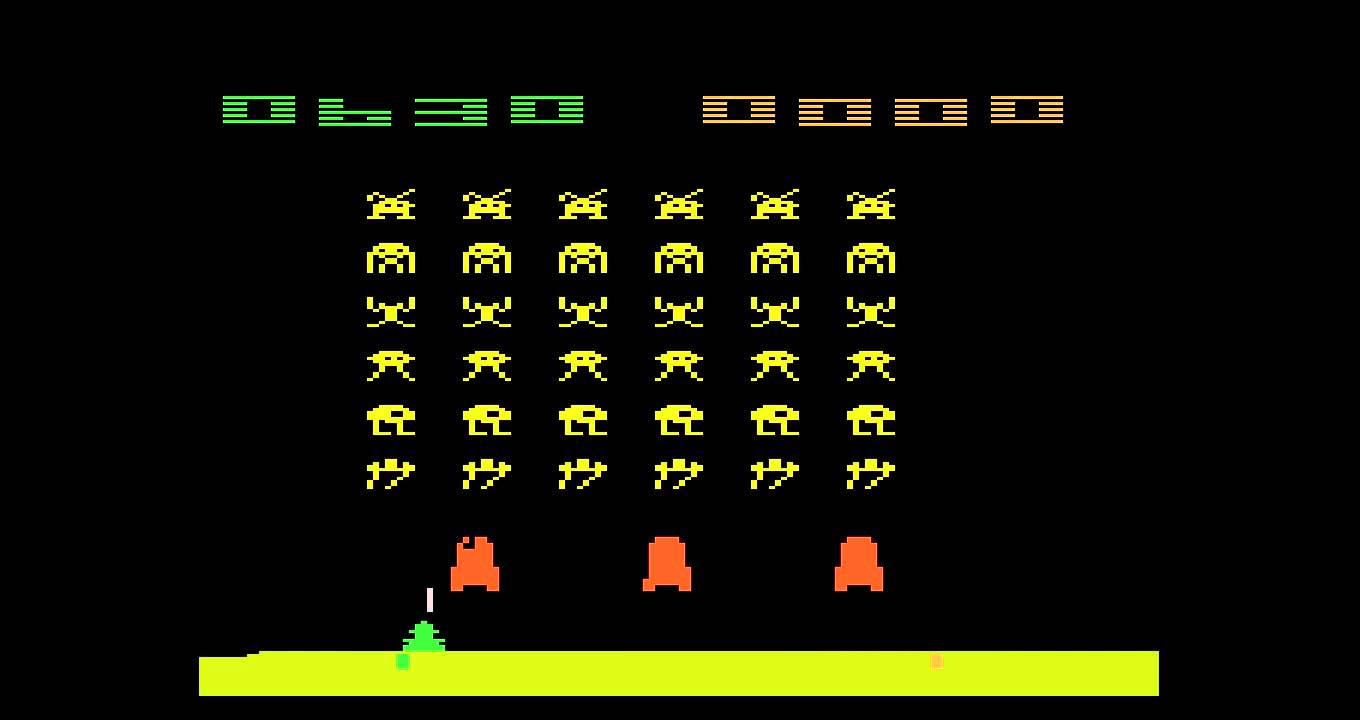
\includegraphics[width=\linewidth]{space_invaders.jpg}
  \caption{A frame form the video game Space Invaders }
  \label{fig:space_invaders}
\end{figure}
\subsection{Value distributions}
One of the major principles of RL states that, if not not otherwise constrained in its behavior, an agent should aim to maximize its expected utility Q, or value~\cite{Sutton:1998:IRL:551283} and as discussed before this is expressed elegantly with the Bellman Operators.\par
Bellemare et al. ~\cite{DBLP:journals/corr/BellemareDM17} argue for the fundamental importance of the value distribution:  the distribution of the random return received by a reinforcement learning  agent. There is a large body of literature on this distribution~\cite{jaquette1973}~\cite{articleSobel} , but for mainly specific purposes, such as implementing risk-aware behavior~\cite{Morimura:2010:NRD:3104322.3104424} or to model parametric uncertainty~\cite{Dearden98bayesianq-learning}. Specifically we are interested on the random return $Z$.\par
\subsection{Distribution Distance Measures}
In this section we will review some  measures of distance between distributions which will be used in this thesis.
\subsubsection{KL Divergence}
In \emph{mathematical statistics}, the Kullback–Leibler divergence (also called relative entropy) is a measure of how one probability distribution is different from a second, reference probability distribution ~\cite{Kullback59}. In the simple case, a Kullback–Leibler divergence of 0 indicates that we can expect similar, if not the same, behavior of two different distributions, while a Kullback–Leibler divergence larger than 0 indicates that the two distributions behave differently and its value indicates ``how much'' the distributions differ. In simplified terms, it is a measure of surprise. 
\par More formally, given two probability measures, $P$ and $Q$, the KL divergence of $Q$ to $P$, $d_{KL}(P,Q)$ is defined as:
\begin{equation}
d_{KL}(P,Q)=\mathbb{E}_{P}\left[\log\frac{P(z)}{Q(z)}\right].
\end{equation}
$d_{KL}(P,Q)$ is an index of the information gained when one revises one's beliefs from the prior probability distribution $Q$ to the posterior probability distribution $P$. In other words, it is the amount of information lost when $Q$ is used to approximate $P$ ~\cite{BurnhamModelSelection}. In applications, $P$ typically represents the ``true'' distribution of data, observations, or a precisely calculated theoretical distribution, while $Q$ typically represents a theory, model, description, or approximation of $P$. In order to find a distribution $Q$ that is closest to $P$, we can minimize KL divergence and compute an information projection.
\subsubsection{Wasserstein Metric}
The Wasserstein metric, $d_p$ is a \emph{distance function} defined between cumulative distributions functions ~\cite{bootstrapAsymptotic}. Given $F$ and $G$, two \emph{c.d.fs}, the Wasserstein metric is defined as:
\begin{equation}
	d_p(F,G)= \inf_{U,V}\Vert U-V\Vert_p,
\end{equation}  
where the infimum is taken over all pairs of random variables $(U,V)$, with respective cumulative distributions $F$ and $G$. For $p< \infty$, and if $U$ and $V$ are defined over $\mathbb{R}$, $d_p$ can be written as:
\begin{equation}
	d_p(F,G)=\left(\int_{0}^{1} |F^{-1}(u)-G^{-1}(u)|^p du \right)^{\frac{1}{p}}.
\end{equation}
Given two random variables $U,V$ with c.d.fs $F_U,F_V$, we will write $d_p(U,V)=d_p(F_U,F_V)$ for convenience.\par
Considering a scalar $a$ and a random variable $A$, independent of $U,V$, the metric $d_p$ has the following properties ~\cite{DBLP:journals/corr/BellemareDM17}:
\begin{equation*}
\begin{split}
		d_p(aU,aV) & \leq \vert a \vert d_p{U,V}, \\
		d_p(A+U,A+V) &  \leq d_p(U,V) \\,
		d_p(AU,AV) & \leq \Vert A \Vert d_p(U,V).
\end{split}
\end{equation*}
Let $\mathcal{Z}$ denote the space of value distributions. For two value distributions $Z_1, Z_2 \in \mathcal{Z}$ a maximal form of the Wasserstein metric can be defined as: 
\begin{equation}
	\overline{d}_p(Z_1,Z_2)= \sup_{s,a} d_p(Z_1(s,a),Z_2(s,a)).
\end{equation}
\subsection{Policy Evaluation Setting}
We recall that agent following a policy $\pi$ in an uncertain world will experience return $Z^\pi$, defined as the sum of discounted rewards following the trajectory induced by policy $\pi$. The value function $Q^\pi$  describes the expected return  from taking  action $a$  in state $s$, then acting according to $\pi$.
\begin{equation*}
	Q^\pi(s,a)=\mathbb{E}\left[Z^\pi(s,a)\right]=\mathbb{E}\left[\sum_{t=0}^{\infty} \gamma^{t}R(s_t,a_t) \right].
\end{equation*}
We emphasize that $Z^\pi$ describes the intrinsic randomness of the agent's interactions with its environment, rather than some measure of uncertainty about the environment itself~\cite{DBLP:journals/corr/BellemareDM17}. We discussed before how this expectation can be expressed elegantly using Bellman's expectation equation. Now we will take away the expectations in Bellman's equation and use the distribution $Z^\pi$\par
The randomness in the return of the next state can also be expressed in the transition operator $P^\pi: \mathcal{Z \rightarrow Z}$, defined as:
\begin{equation}
\begin{aligned}
	P^\pi Z(s,a) \,{\buildrel D \over =}\ Z(S',A') \\
	S' \sim P(\cdot |s,a) \quad A' \sim \pi(S'),
\end{aligned}
\end{equation} 
where $\,{\buildrel D \over =}\ $ is an equality in distribution. We use the capital letters $S'$ and $A'$ to emphasize the random nature of the next state-action pair. Now we can give the definition of the distributional Bellman operator, $\mathcal{T}^\pi Z \rightarrow Z$, as 
\begin{equation}
	\mathcal{T}^\pi Z(s,a) \,{\buildrel D \over =}\ R(s,a)+ \gamma P^\pi Z(s,a).
	\label{eq:bellman_distributional}
\end{equation} 
The \emph{distributional Bellman operator} states that the distribution of $Z$ is characterized by the interaction of three random variables: 
\begin{itemize}
	\item the reward $R$;
	\item the next state-action ($S',A'$);
	\item the random return in the next state-action. $Z(S',A')$
\end{itemize}
Further it can be shown that equation ~\ref{eq:bellman_distributional} is a contraction mapping in Wasserstein metric and its unique fixed point is $Z^\pi$~\cite{DBLP:journals/corr/BellemareDM17} 
\begin{equation}
	\overline{d}_p(T^{\pi}Z_1,T^{\pi}Z_2) \leq \gamma \overline{d}_p(Z_1,Z_2).
\end{equation}
In  this  context,  the  Wasserstein metric is particularly interesting because it does not suffer from disjoint-support issues ~\cite{pmlr-v70-arjovsky17a} which  arise  when  performing  Bellman  updates.
\subsection{The Control Setting}
In the previous section we discussed how the Bellman distributional operator has the same properties as the expectation one. This does not hold in the control setting unfortunately, with the optimality operator. As a reminder, in the control setting we seek a policy $\pi$ that maximizes the value function and the corresponding notion of an optimal value distribution. We will see how optimality is a trickier concept when seen in a distributional setting.Just like with the value function, the notion of optimal value distribution is tied with the notion of an optimal policy. But if with value functions , all optimal policies have the same optimal value function , this is not the case with value distributions. \par
The notion of optimal policy does not change. The optimal policy is still the policy that maximizes the expected return. Having the definition of the optimal policy , we can define the optimal value distribution as :
\begin{definition}
	An optimal value distribution is the value distribution of an optimal policy. The set of optimal value distributions is  $\mathcal{Z^*} := \left\lbrace \mathcal{Z^{\pi^*}} : \pi^* \in \Pi^* \right\rbrace$
\end{definition}
We emphasize that not all value distributions with expectation $Q^\pi$ are optimal. They must match the full distribution  of the return under some optimal policy.\par
Recall that the expected Bellman optimality operator $\mathcal{T}$. In (~\ref{eq:bellman_optimality}) the maximum over actions corresponds to an implicit greedy policy, which cannot be ignored in the distributional case. So let us give the definition of a greedy policy as provided by ~\cite{DBLP:journals/corr/BellemareDM17}.
\begin{definition}
	A greedy policy $\pi$ for $Z \in \mathcal{Z}$ maximizes the expectation of $Z$. The set of greedy policies for $Z$ is:
	\begin{equation*}
	\mathcal{G}_{Z} = \left\lbrace \pi : \sum_{a \in \mathcal{A}} \pi(a|s) \mathbb{E}\left[Z(s,a)\right] =\max_{a' \in \mathcal{A}} \mathbb{E} \left[Z(s,a')\right] \right\rbrace.
	\end{equation*}
\end{definition}
After defining the notion of a greedy policy we can define a distributional optimality operator as any operator $\mathcal{T}$ which implements a greedy selection rule, \ie
\begin{equation}
	\mathcal{T}Z=\mathcal{T}^\pi Z \quad for \quad some \quad \pi \in \mathcal{G}_{Z}.
\end{equation}
 As in the policy evaluation setting, we are interested in the behavior of the iterates $Z_{k+1}= \mathcal{T}Z_k$ where $Z_0 \in \mathcal{Z}$. Bellemare ~\cite{DBLP:journals/corr/BellemareDM17} shows that the expectation, $\mathbb{E}Z$ behaves as expected, converging to $Q^*$ exponentially quickly. Unfortunately, convergence of $Z_k$ to $Z^*$ is neither quick nor assured to reach a fixed point. In Bellemare derives 3 negatives results concerning the operator $\mathcal{T}$:
 \begin{itemize}
 	\item The operator $\mathcal{T}$ is not a contraction in any measure;
 	\item Not all optimality operator have a fixed point $Z^*$;
 	\item Even if $\mathcal{T}$ has a fixed point, it does not guarantee the convergence of $\lbrace Z_k\rbrace$ to $\mathcal{Z^*}$.
 \end{itemize} 
\chapter{State of The Art in Efficient Exploration} \label{chap:chapter3}
A fundamental issue in reinforcement learning algorithms is how to balance between exploration of the environment and exploitation of information already obtained by the agent. There is a large body of literature on efficient exploration tackling the exploration vs exploitation dilemma. The goal of exploration strategies is minimizing learning time while providing some guarantees on the performance of the learned policy. Clearly, the more effectively and efficiently an agent explores and learns from its environment, the more effectively and efficiently it uses its time, and hence, the less time is required for learning. Intuitively, one might infer that pure exploration during learning would be the most effective learning approach. However, this is not the case. Pure exploration may waste much time and computing resources exploring task-irrelevant parts of the environment. This also means that the agent's performance during learning will be poor, relatively speaking, since it spends some unnecessary portion of its time performing actions that do not help it in achieving its goals. \par
It is often advantageous to find some suitable balance of both exploration and exploitation. If the agent can exploit its current knowledge of the environment, it may be able to identify the most worthwhile parts of the environment to explore. Further, minimizing the learning costs (\ie maximizing the agent's performance during learning) cannot be done without some degree of exploration of the environment such that effective behaviours can be discovered. 
Another problem that may arise is the applicability of the exploration strategy to the task at hand. An exploration strategy that performs well in one environment may be ill suited to another environment. Thrun in ~\cite{Thrun92efficientexploration} observed that the impact of the exploration technique on both learning time and learning costs can be enormous. \par
The purpose of this chapter is to review some relevant algorithms in the field of efficient exploration, starting from the classical ones to the more modern ones. In Section ~\ref{exploration} reviews measures of efficient exploration and some algorithms that give theoretical guarantees. Section ~\ref{deep_exploration} describes deep exploration and Bootstrapped DQN as an example algorithm that performs deep exploration. Finally, Section ~\ref{distributional_rl} is devoted to algorithms that perform exploration using the value distribution, and the distributional Bellman operator.
\section{Exploration} \label{exploration}
\subsection{Measuring Efficient Exploration}
Before reviewing the state of the art in exploration, it is important to discuss how to measure the efficiency of an RL algorithm in formal terms. In this section we will review two important measures, \emph{sample complexity} and \emph{regret}.
\subsubsection{Sample Complexity}
Sample complexity defined as the time required by the algorithm to find an approximately optimal policy ~\cite{Gatsby2003OnTS}. More formally:
\begin{itemize}
 \item Let $\mathcal{M}$ be an MDP with N states, K actions, discount factor $\gamma$ and a maximal reward $R_{max}$ >0;
 \item Let A be an algorithm that acts in the environment producing experience $s_0$, $a_0$, $r_1$, $s_1$, $a_1$, $r_2$ $\ldots$;
 \item Let $V^{A}_t=\mathbb{E} \left[ \sum_{\tau =0}^{\infty} \gamma^\tau r_{t+\tau} \mid s_0,a_0,r_1 \ldots s_{t-1},a_{t-1},r_t,s_t \right]$ be the value accumulated by A;
 \item Let $V^*$ be the value function of the optimal policy;
\end{itemize}
\begin{definition}
	Let $\epsilon > 0 $ be a prescribed accuracy and $\delta > 0$ be an allowed probability of failure. The expression $\eta(\epsilon,\delta,N,K,\gamma,R_{max})$ is a sample complexity bound for algorithm A if independently of the choice of $s_0$,with probability at least $1-\delta$, the time steps such that $V^{A}_t < V^* - \epsilon$ is at most $\eta(\epsilon,\delta,N,K,\gamma,R_{max})$.
\end{definition}
Now that we have a measure of the efficiency of RL algorithms, we can give the definition of \emph{PAC-MDPs}, a class of algorithms which includes some of the algorithms we will discuss further.
\begin{definition}
An algorithm with sample complexity that is polynomial in $\frac{1}{\epsilon}$, $\log\frac{1}{\delta}$, $N$, $K$, $\frac{1}{1-\gamma}$, $R_{max}$ is called PAC-MDP (probably approximately correct in MDPs).
\end{definition}
\subsubsection{Regret}
Regret is defined as the difference between the cumulative reward of the optimal policy and that gathered by the policy $\pi$ played by the agent hence is usually used with on-policy algorithms. More formally, the total regret of policy $\pi$ after $T$ steps, $R^{\pi}(T)$ is defined as:
\begin{equation}
	R^{\pi}(T)=\sum_{t=1}^{T}\left(V^{\pi^*}(s_t^{\pi^*})-V^{\pi^t}(s_t^{\pi})\right),
\end{equation}
where $s_t^{\pi^*}$ is the state the agent would have been in time step $t$, if he had followed optimal policy $\pi^*$. Regret measures the cumulative reward loss due to the need of learning, quantifying the exploration vs. exploitation dilemma. 
\subsection{Explicit Explore or Exploit}
In the previous chapter we shortly reviewed the Q-Learning algorithm. An important characteristic of Q-learning is that it is a model-free approach to learning an optimal policy in an MDP with unknown parameters. In other words, there is not an explicit attempt to model or estimate costs and/or transition probabilities, the value of each action is estimated directly through samples. Another approach to the same problem is to estimate the MDP parameters from the data and find a policy based on the estimated parameters (model-based). In this sections, we will review an algorithm of that class specifically designed for efficient exploration, the Explicit Explore or Exploit ($E^3$) algorithm, proposed by Kearns and Singh ~\cite{Kearns:2002:NRL:599616.599699}. $E^3$ is a model-based, PAC-MDP algorithm which assumes knowlwdge of the maximum reward of the MDP and uses the concept of \emph{optimism in the face of uncertainty}.\par 
The main ideas of $E^3$ are as follows :
\begin{itemize}
	\item The state space $S$ is divided in two parts, \emph{known states} $N$ and \emph{unknown states} $N^C$,
	\item Counters for state and actions are kept to quantify confidence in model estimates,
	\item Known states have been visited sufficiently many times to guarantee that the transition probabilities $P(s,a,s')$ and rewards $R(s,a,s')$ are accurate with high probabilities for every tuple $(s,a,s') \in S \times A \times S$,
	\item Unknown states are moved to the known set, $N$, when they are visited at least $m$ times, for some number $m$.
\end{itemize}
By separating the state space in two subsets, $E^3$ defines two different MDPs. The first MDP, $MDP_{known}$, includes the states in the set N and the calculated values for the transition probabilities and Reward function. This MDP is used for exploitation. The second MDP, $MDP_{unknown}$, has the same structure as the first one with the addition of a special state $s'$ which includes all the unknown states and the reward for reaching it is maximal, for every action $a \in A$. Pseudocode of the $E^3$ algorithm is shown in Alg.~\ref{alg:e3}
\begin{algorithm}[H]
\begin{flushleft}
 \textbf{Input:} $s$ - Current state\\
 \textbf{Output:} $a$ -Action to execute
\end{flushleft}
 \begin{algorithmic}
 
 \If{$s$ is known }
 \State Plan in $MDP_{known}$
 \If{resulting plan has value above some threshold}
 \State \Return first action of plan
 \Else
 	 \State Plan in $MDP_{unknown}$
 	 \State \Return first action of plan
 \EndIf
 \Else
 	\State \Return action with the least observations in $s$
 \EndIf
 \end{algorithmic}
 \caption{$E^3$ algorithm}
 \label{alg:e3}
\end{algorithm}
$E^3$ makes the exploitation vs exploration dilemma explicit by choosing in which of the two MDPs to plan, based on the confidence it has on the model parameters estimated so far. Kearns and Singh ~\cite{Kearns:2002:NRL:599616.599699} show that, with probability no less than $1-\delta$, $E^3$ will stop after a number of actions and computation time $poly(\frac{1}{\epsilon},\frac{1}{\delta},N,\frac{1}{1-\alpha},R_{max})$. The number of samples required to solve the MDP is polynomial in the number of states, so the algorithm is called efficient. However, in natural environments, the number of states is enormous, exponential to the number of state variables. This makes $E^3$ exponential in the number of states variables. 
\subsection{R-Max}
R-max is a very simple model-based reinforcement learning algorithm which can attain near-optimal average reward in polynomial time. In R-max, the agent always maintains a complete, but possibly inaccurate model of its environment and acts based on the optimal policy derived from this model. The model is initialized in an optimistic fashion: all actions in all states return the maximal possible reward (hence the name). During execution, it is updated based on the agent's observations.
R-max improves upon several previous algorithms: (1) It is simpler and more general than Kearns and Singh’s $E^3$ algorithm, covering \emph{zero-sum stochastic games}. (2) It has a built-in mechanism for resolving the exploration vs. exploitation dilemma. (3) It formally justifies the \emph{optimism under uncertainty} bias used in many RL algorithms. (4) It implicitly addresses the exploration vs exploitation dilemma.\par
\subsubsection{Stochastic Games}
Before explaining how R-max works, it is important to shortly define the framework of stochastic games. We consider a stochastic game $\mathcal{M}$ consisting of a set $\mathcal{S}= \lbrace G_1,\ldots,G_N \rbrace$ of stage-games in which both the agent and the adversary, have a set $\mathcal{A}= \lbrace a_1,\ldots,a_K \rbrace$ of possible actions. We associate a reward matrix $R^i$ with each game, and use $R^i_{m,l}$ to denote a pair consisting of the reward obtained by the agent and the adversary after playing actions $a_m$ and $a_l$ in game $G_i$, respectively. In addition, we have a probabilistic transition function, $P_M$, such that $P_M(s,t,a,a')$ is the probability of making a transition from $G_s$ to $G_t$ given that the agent played $a$ and the adversary played $a'$. This way, all model
parameters, both rewards and transitions, are associated with joint actions of a particular game.
\subsubsection{R-max algorithm}
In R-max, the agent will always attempt to optimize its behavior, albeit with respect to a fictitious model. Roughly speaking, this model assumes that the reward the agent obtains in any situation it is not too familiar with is its maximal possible reward, denoted by $R_{max}$. Often, optimal behavior with respect to this fictitious
model results in exploration with respect to the real model, and thus, to learning. The
major insight behind the R-max algorithm is that the optimal policy with respect to the agent’s fictitious model has a very interesting and useful property with respect to the real model: it is always either optimal or it leads to efficient learning. In many situations, the agent will not know ahead of time whether its behavior will lead to optimizing behavior with respect to the real model or to learning – this depends on how the adversary will act. However, it knows that it will either optimize or learn efficiently.\par
The approach taken by R-max is not new. It has been referred to as the optimism in the face of uncertainty heuristic, and was considered an ad-hoc, though useful, approach ~\cite{KLMSurvey,Sutton:1998:IRL:551283}. The approach has been extensively studied in the framework of multi armed bandits ~\cite{journals/corr/abs-1204-5721}. This optimistic bias has also been used in a number of well-known reinforcement learning algorithms, e.g. Kaelbling’s interval exploration method ~\cite{kaelbling1993learning}, the exploration bonus in Dyna ~\cite{DBLP:journals/sigart/Sutton91} etc. However, none of this work provides theoretical justification for this very natural bias. Brafman and Tennenholtz ~\cite{Brafman:2003:RGP:944919.944928} provide a formal justification for the optimism under uncertainty bias, used in their R-max algorithm.\par
The algorithm is quite simple. Model $\mathcal{M}'$ is constructed, containing the set of $N+1$ games $\mathcal{S}= \lbrace G_0,G_1,\ldots,G_N \rbrace$, where $G_0$ is an initial fictitious game, and the set of $k$ actions $\mathcal{A}= \lbrace a_1,\ldots,a_K \rbrace$. The reward matrices are initialized to have ($R_{max},0$) in all entries whereas the transition model is initialized $P_M(G_i,G_0,a,a′)$ = 1 for all i=$0,\ldots,N$ and for all actions $a,a′$. In addition, for each game, we maintain some additional information:
\begin{itemize}
\item a boolean value depicting whether the state is \emph{known} or \emph{unknown}, initiliazed to unknown;
\item the states reached by playing the joint action corresponding to this entry (and how many times each state was reached), initially empty;
\item the reward obtained (by both players) when playing the joint action
corresponding to this entry, initially empty.
\end{itemize}
The algorithm assumes knowledge of the maximum reward, $R_{max}$, and the $\epsilon$-return mixing time of an optimal policy, $T$. After the initialization phase the algorithm enters its main loop, composed of two phases. The first phase called \emph{Compute and Act}, computes an optimal $T$ -step policy for the current state, and executes it for $T$-steps or until a new entry becomes known. The second phase, \emph{Observe and update}, follows each joint action as follows: Let $a$ be the action the agent performed in $G_i$ and let $a'$ be the adversary's action:
\begin{itemize}
\item If the joint action ($a,a'$) is performed for the first time in $G_i$, update the reward associated with ($a,a'$) in $G_i$, as observed;
\item Update the set of states reached by playing ($a,a′$) in $G_i$ ;
\item If at this point your record of states reached from this entry contains \\ $K_1=\max \left( \lceil (\frac{4NTR_{max}}{\epsilon})^3 \rceil,\lceil -6 \ln^3(\frac{\delta}{6Nk^2}) \rceil \right) +1$ elements, mark this entry as known and update the transition probabilities for this entry according to the observed frequencies.
\end{itemize}
R-max starts with an initial estimate for the model parameters that assumes all states and all joint actions yield maximal reward and lead with probability 1 to the fictitious stage-game $G_0$. Based on the current model, an optimal $T$-step policy is computed and followed. Following each joint action the agent arrives at a new stage-game, and this transition is recorded in the appropriate place. Once we have enough information about where some joint action leads to from some stage-game, we update the entries associated with this stage-game and this joint action in our model. After each model update, we recompute an optimal policy and repeat the above steps.\par
Like $E^3$, R-max is a model based approach, meaning that it maintains a model of the environment and uses the samples of experience to estimate the model parameters and uses the latter to plan in the environment. Unlike $E^3$, exploration is done implicitly due to the initialization of the reward matrices at R-max, meaning that unknown states will explored since the model gives high reward for them. Another point in common is the efficiency of the algorithm. R-max is also PAC-MDP, meaning that the number of samples needed to find the optimal policy scales polynomially with respect to the number of states, which again wields a exponential complexity with respect to the state variables.
\subsection{Upper Confidence Reinforcement Learning}

\subsubsection{UCRL}
Upper Confidence bound Reinforcement Learning (UCRL)~\cite{NIPS2006_3052} tries to apply the standard optimism in face of uncertainty in the RL context, by selecting optimistic policies consistent with some confidence set over the MDPs. UCRL is again a model-based algorithm that uses the optimism in face of uncertainty principle to plan over the model it has estimated. To select good policies, the agent keeps track of estimates for the average rewards and the transition probabilities as follows:
\begin{itemize}
\item $N_t(s,a)$ being the number of times action $a$ was chosen in state $s$,
\item $R_t(s,a)$ being the sum of rewards collected when choosing action $a$ in state $s$,
\item $P_t(s,a,a')$ being the number of times the agent transitioned to state $s'$ from state $s$, executing action $a$. 
\end{itemize}\
From these number we can get estimates of the reward and transitions probabilities:
\begin{equation}
	\hat{r}_t(s,a)=\frac{R_t(s,a)}{N_t(s,a)},
\end{equation}
\begin{equation}
	\hat{p}_t(s,a,s')=\frac{P_t(s,a,a')}{N_t(s,a)},
\end{equation}
provided that the state counter in $(s,a)$, $N_t(s,a)$>0. Together with appropriate confidence intervals, these estimates may be used to define a set $\mathcal{M_t}$
of plausible MDPs. UCRL then chooses an optimal policy $\pi_t$ for an MDP $M_{t}$ with maximal average reward $\rho^{∗}_t$=$\rho^*(M_t)$ where $\rho^*(M_t)$ is the \emph{average reward} of the optimal policy in MDP $M_t$. That is:
\begin{equation}
	\rho^*(M)=\rho(M,\pi^*)=\sum_{s\in S} \mu_{\pi^*}(s) r(s,\pi^*(s)),
\end{equation}
where $\mu_{\pi^*}$ is the stationary distribution induced by $\pi^*$ in $M$.\par
UCRL includes in the set $\mathcal{M}_t$ those MDPs $M'$ whose transition probabilities $p'(\cdot,\cdot,\cdot)$, and rewards $r'(\cdot,\cdot)$ satisfy for all states $s,s'$ and actions $a$:
\begin{equation}
		r'(s,a)\leq \hat{r}_t(s,a) +\sqrt{\frac{\log(2t^\alpha |S| |A|)}{2N_t(s,a)}},
\end{equation}
\begin{equation}
		|p'(s,a,s')- \hat{p}_t(s,a,s')| \leq \sqrt{\frac{\log(4t^\alpha |S|^2 |A|)}{2N_t(s,a)}},
\end{equation}
for some $\alpha>2$. The intuition behind the algorithm is that if a non-optimal policy is followed, then this is eventually observed and something about the MDP is learned. Auer and Ortner ~\cite{NIPS2006_3052} show that this learning happens sufficiently fast to approach an optimal policy with only logarithmic regret. As switching policies too often may be harmful, and estimates do not change very much after few steps, UCRL discards the policy $\pi_t$ only if there was considerable progress concerning the estimates of the transition model or reward. That is, UCRL sticks to a policy until the length of some of the confidence intervals given before is halved. Only then a new policy is calculated.

\subsubsection{UCRL2}
We will now review a variant of UCRL algorithm discussed in the previous section. As its predecessor, UCRL2 ~\cite{Jaksch:2010:NRB:1756006.1859902} implements the paradigm of optimism in the face of uncertainty. That is, it defines a set $\mathcal{M}$ of statistically plausible MDPs given the observations so far, and chooses an optimistic MDP, $M_t$ (with respect to the achievable average reward) among these plausible MDPs. Then it executes a policy $\pi_t$ which is (nearly) optimal for the optimistic MDP $M_t$. The algorithm proceeds in episodes and computes a new policy $\pi_k$ only at the beginning of each episode $k$, unlike URCL which switched policies based on the size of the confidence interval in each step, compared to the size of the interval when the policy was first calculated. The lengths of the episodes are not fixed a priori, but depend on the observations made.\par
The algorithm computes the estimates for the mean rewards and the transition probabilities from the observations made before episode $k$. As before, a set of plausible MDPs is calculated using slightly different confidence intervals. This guarantees that with high probability the true MDP $M$ is in the set $\mathcal{M}_k$. At this point, UCRL2 adds a new step called \emph{extended value iteration}~\cite{Jaksch:2010:NRB:1756006.1859902} , used to choose a near-optimal policy $\pi_k$ on an optimistic MDP $M_k \in \mathcal{M}_k$. This policy $\pi_k$ is executed throughout episode $k$. Episode $k$ ends when a state $s$ is visited in which the action $a =\pi_k(s)$ induced by the current policy has been chosen in episode $k$ equally often as before episode $k$. Thus, the total number of occurrences of any state-action pair is at most doubled during an episode. The algorithm has to keep tack of these counters also. UCRL2 improves the regret bounds of its predecessor. 
\subsection{Delayed Q Learning}
We will now discuss Delayed Q-Learning ~\cite{Strehl:2006:PMR:1143844.1143955}, a PAC-MDP, model-free RL algorithm. We recall that the algorithms reviewed so far in this chapter, while being PAC-MDP, were model-based. They explicitly estimate the model of the MDP and then take decisions based on the model and their confidence about it.\par Delayed Q-Learning does not maintain estimates of the model parameters. The algorithm keeps Q-value estimates, $Q(s,a)$, for each state action pair $(s,a)$. In addition to these estimates, the algorithm maintains boolean flags associated to each state-action pair, $LEARN(s,a)$. The value of the flag at time $t, LEARN_t(s,a)$, denotes whether the agent is considering a change to its Q-value estimate $Q(s_t,a_t)$. A counter, $l(s,a)$, is also maintained for each $(s,a)$ pair. The counter represents the amount of samples acquired for use in an upcoming update of $Q(s,a)$. Two additional parameters are required, $\epsilon_1 \in [0,1]$ and a positive integer $m$. The algorithm is initialized as follows:
\begin{itemize}
	\item The Q-value estimates, $Q(s,a)$, are initialized at $\frac{1}{1-\gamma}$ for all $(s,a) \in S \times A$ (it is assumed $R(s,a) \in [0,1]$),
	\item The counters, $l(s,a)$, are initialized at zero for all $(s,a) \in S \times A$,
	\item The flags, $LEARN(s,a)$, are initialized a $true$ for all $(s,a) \in S \times A$.
\end{itemize}\par
We will now discuss the update rule of Delayed Q-Learning. At time step $t$, the agent is at state $s$ and performs action $a$. If the value of the counter, $l(s,a)$, is larger than the parameter $m$, the transition results in an \emph{attempted update}. Let $s_{k_1}, s_{k_2}, \ldots, s_{k_m}$ be the $m$ most recent next-states observed from executing $(s, a)$, at times $k_1< k_2 < \ldots < k_m$, respectively ($k_m=t$), and $r_i$ the $i-th$ reward received during execution of Delayed Q-learning. Thus, at time $k_i$, action $a$ was executed at state $s$, resulting in a transition to state $s_{k_i}$ and receiving reward $r_{k_i}$. At this point the following update rule is considered:
\begin{equation}
	Q_{t+1}(s,a)=\frac{1}{m}\sum_{i=1}^{m}(r_{k_i}+ \gamma V_{k_i}(s_{k_i})) +\epsilon_1.
\end{equation}
The update is performed as long as the new value is at least $\epsilon_1$ smaller than the previous estimate (hence attempted update). In other words the following condition must be satisfied:
\begin{equation}
	Q_t(s,a)- \frac{1}{m}\sum_{i=1}^{m}(r_{k_i}+ \gamma V_{k_i}(s_{k_i})) >=2 \epsilon_1.
\end{equation}
If the condition does not hold, or the $LEARN(s,a)$ flag is $false$ the update is not performed and $Q_{t+1}(s,a)=Q_t(s,a)$. The flags are initialized to true, and they are changed to false only when no updates are made during a length of time for which ($s, a$) is experienced $m$ times and the next attempted update of $(s, a$) fails. In this case, no more attempted updates of ($s, a$) are allowed until another Q-value estimate is updated, time when all flags are set to $true$, because the update might need to propagate to other state action pairs.\par
Delayed Q-learning is similar to traditional Q-Learning. In fact, if we used learning rate, $\alpha_t=\frac{1}{(l_t(s,a)+1)}$, then $m$ repetitions of the Q-learning update would be similar to the Delayed Q-Learning update, minus a small bonus of $\epsilon_1$. The difference is that Q-Learning performs updates in every step whereas the former waits for $m$ samples to perform an update. This delay has an averaging effect, which removes some of the effects of randomness, and combined with the $\epsilon_1$ bonus, achieves an optimism ($Q(s,a)>Q^*(s,a))$ with high probability ~\cite{Strehl:2006:PMR:1143844.1143955}. The property of optimism is useful for efficient exploration and appears in many RL algorithms. The intuition is that if an action’s Q-value is optimistic the agent will learn much by executing that action. Since the action-selection strategy is greedy, the Delayed Q-learning agent will tend to choose overly optimistic actions, therefore achieving directed exploration when necessary. If sufficient learning has been completed and all Q-values are close to their true $Q^*$ values and selecting the maximum will guarantee near-optimal behavior.
\subsection{Bayesian Q Learning}
Dearden et al.~\cite{Dearden98bayesianq-learning} apply a Bayesian approach to tackle the exploration vs exploitation dilemma. They extend Q-Learning by maintaining and propagating probability distributions over the Q-values. By maintaining these distributions over the Q-values, rather than just point estimates, we are able to make more informed decisions.\par
In the Bayesian framework, we need to consider \emph{prior} distributions over Q-values, and then update these priors based on the collected experience. Let $R_{s,a}$ be a random variable denoting the total discounted reward received when executing action $a$, starting from state $s$, and then following an optimal policy. We are uncertain of how $R_{s,a}$ is distributed. Dearden et al. make a number of assumption in their paper:
\begin{itemize}
	\item $R_{s,a}$ has a normal distribution. By making these assumption we are able to model the uncertainty over the distribution by modeling a distribution over the mean $\mu_{s,a}$ and \emph{precision}, $\tau_{s,a}$.
	\item The prior distribution over $\mu_{s,a}$ and $\tau_{s,a}$ is independent from the prior distribution over $\mu_{s',a'}$ and $\tau_{s',a'}$ for $s \neq s'$ or $a \neq a'$.
	\item The prior $p(\mu_{s,a},\tau_{s,a})$ is a \emph{normal-gamma} distribution ~\cite{degroot2012probability}, determined by a tuple of hyperparameters, $\rho=(\mu_0,\lambda,\alpha,\beta)$. The choice of the normal-gamma distribution to represent the normal distribution of $R_{s,a}$ with unknown mean $\mu_{s,a}$ and precision $\tau_{s,a}$, is important because standard results ~\cite{degroot2012probability} show that the posterior of a normal-gamma distribution is again a normal-gamma distribution. This mean that to represent the agent's prior over the distribution of $R_{s,a}$ we need only to maintain the tuple $\rho_{s,a}=(\mu_0^{s,a},\lambda^{s,a},\alpha^{s,a},\beta^{s,a})$ for all $(s,a) \in \mathcal{S \times A}$.
	\item At any stage, the agent's posterior over $\mu_{s,a}$ and $\tau_{s,a}$ is independent from the posterior distribution over $\mu_{s',a'}$ and $\tau_{s',a'}$ for $s \neq s'$ or $a \neq a'$.
\end{itemize} 
\subsubsection{Action Selection}
Bayesian Q-Learning uses this compact representation in a similar way to Q-Learning, but instead of storing the Q-values, it stores the hyperparameters of the distributions. Using the distributions, Bayesian Q-Learning uses to different methods to perform action selection. The first method uses \emph{Q-value sampling}, first described by Wyatt ~\cite{articleWyatt1997}. The idea is to select actions stochastically, based on the probability that actions are optimal. To do this we can use the distributions to calculate the probability for each action to be optimal. To avoid the calculation of this probability, in practice we sample from the distribution of each action and execute the action with maximum sample value. One drawback of this selection method is that it only considers the probability of action $a$ to be optimal, and does not take into account how much this action improves over the current policy. Figure \ref{fig:q_value_sampling} shows an example where even though Q-value sampling would give the same result, the benefit of exploring action $a_2$ is larger in the second case since the probability to experience higher rewards is higher.\par
\begin{figure}
 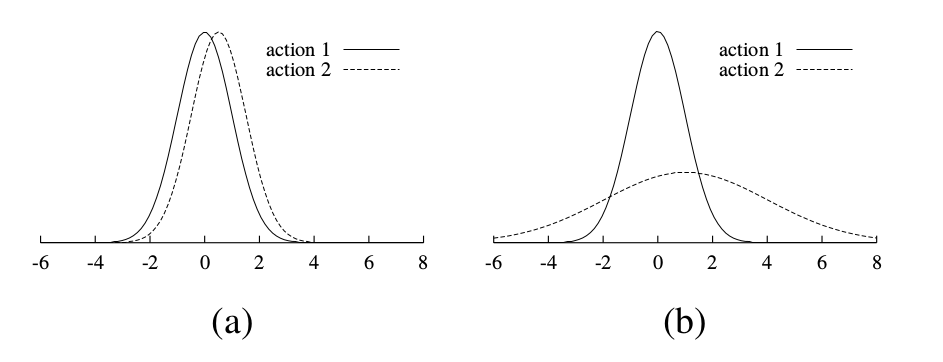
\includegraphics[width=\linewidth]{q_value_sampling.png}
 \caption{Examples of Q-value distributions of two actions for which Q-value sampling has the same exploration policy even though the payoff of exploration in (b) is higher than in (a) ~\cite{Dearden98bayesianq-learning}.}
 \label{fig:q_value_sampling}
\end{figure}
The second method of action selection is \emph{Myopic-VPI}. This method uses the distributions over the Q-values to calculate an approximation of the \emph{Value of Information} ~\cite{4082064} for each action and then selects the action that best balances exploration and exploitation according to the criterion. The idea is to balance the expected gains from exploration, in the form of improved policies, against the expected cost of doing a potentially suboptimal action. The only interesting scenarios are those where the new knowledge collected from exploration does change the agent’s policy. This can happen in two cases: 
\begin{itemize}
\item When the new knowledge shows that an action previously considered sub-optimal is revealed as the best choice (given the agent’s beliefs about other actions),
\item When the new knowledge indicates that an action that was previously considered best is actually inferior to other actions.
\end{itemize}
Based on the above logic, Dearden et al. derive closed form equations to calculate the VPI for each action, and execute the action that maximizes: 
\begin{equation}
	\mathbb{E}[Q(s,a)]+VPI(s,a).
\end{equation}
The value of exploration estimate is used as a way of boosting the desirability of different actions. When the agent is confident of the estimated Q-values, the VPI of each action is close to 0, and the agent will always choose the action with the highest expected value.
\subsubsection{Updating the Distribution}
The question of updating the distributions maintained it is complicated due to the fact that we maintain the distribution of Q-values, which are the expected total discounted reward, whereas the observations available are samples of the local reward\footnote{In this sense BQL is a distributional approach.}. For this reason, standard Bayesian results cannot be used directly. Suppose the agent is at state $s$, executes action $a$, observes next-state $s'$ and reward $r$. We would like to know the complete sequence of rewards observed from state $s'$ onward, but unfortunately this is not available. Let $R_{s'}$ be the total sum of discounted rewards collected from $s'$. If the agent will follow the optimal policy then $R_{s'}$ is distributed as $R_{s',a'}$ where $a'$ is the action with highest expected value at $s'$. Bayesian Q-Learning proposes to ways to use this distribution to substitute for the unknown future experiences.\par
The first method proposed is \emph{Moment Updating}. The idea is to sample $R_{s'}^1, \ldots, R_{s'}^n$ from the distribution of the Q-values in the next state, $R_{s',a'}$, and use these values to update $P(R_{s,a})$ with the samples $r+\gamma R_{s'}^1, \ldots, r+\gamma R_{s'}^n$. Dearden et al. show that we need just the first two moments of the distribution to perform the update, which for $n$ that tends to infinity are given by:
\begin{equation}
\label{eq:moment_updating}
\begin{split}
	& M_1= r+\gamma \mathbb{E}[R_{s'}], \\
	& M_2= r^2+2 \gamma r \mathbb{E}[R_{s'}]+ \gamma^2 \mathbb{E}[R_{s'}^2],
\end{split}
\end{equation} 
where $\mathbb{E}[R_{s'}]=\mu_0$ and $\mathbb{E}[R_{s'}^2]=\frac{\lambda+1}{\lambda} \frac{\beta}{\alpha-1}+ \mu_0^2$.
Using (~\ref{eq:moment_updating}) and standard results for normal-gamma distribution ~\cite{degroot2012probability}, Dearden et al. give the posterior $p(\mu_{s,a},\tau_{s,a} | r+\gamma R_{s'}^1, \ldots, r+\gamma R_{s'}^n) \sim NG(\mu_{0_{s,a}}',\lambda_{s,a}',\alpha_{s,a}',\beta_{s,a}')$ where:
\begin{equation}
\begin{split}
	& \mu_{0_{s,a}}'=\frac{\lambda_{s,a} \mu_{0_{s,a}} + M_1}{\lambda_{s,a}+1}, \\
	& \lambda_{s,a}'=\lambda_{s,a}+1, \\
	& \alpha_{s,a}'=\alpha_{s,a}+ \frac{1}{2}, \\
	& \beta_{s,a}'=\beta_{s,a}+\frac{1}{2}(M_2-M_1^2)+ \frac{\lambda_{s,a}(M_1-\mu_{0_{s,a}})^2}{2(\lambda_{s,a}+1)}.
\end{split}
\end{equation}
Moment updating results in a simple closed form solution, but unfortunately becomes to confident of the value of the mean $\mu_{s,a}$. This leads to low exploration values and hence to premature convergence.\par
The second update method proposed is \emph{Mixture Updating}. The method was proposed to avoid the premature convergence problem of Moment Updating. This method uses the distribution of $R_{s'}$ in a slightly different way. Let $p(\mu_{s,a},\tau_{s,a}|R)$ be the posterior distribution after observing discounted reward $R$. If we observed $R_{s'}=x$, we would have the posterior $p(\mu_{s,a},\tau_{s,a}|r+ \gamma x)$. We can capture the uncertainty of the value of $x$, by weighting this distribution with the probability $R_{s'}=x$. This way we get the following \emph{mixture distribution} :
\begin{equation}
	p^{mix}(\mu_{s,a},\tau_{s,a})=\int_{-\infty}^{\infty} p(\mu_{s,a},\tau_{s,a} |r + \gamma x) P(R_{s'}=x) d(x).
\end{equation} 
Unfortunately this distribution is no longer a normal-gamma distribution, and performing this update in every time step would result, each time, in a more complex distribution. Dearden et al. use an approximation to keep the distribution normal-gamma, but unfortunately they did not come with a closed form solution for the update. Performing Mixture update, while it leads to better and more efficient exploration, comes with higher computational effort compared to Moment Updating, as a result of the numericalcalculation of integrals needed to perform the update. \par
Finally, it is important to note that BQL does not guarantee efficient exploration. BQL guarantees convergence of the algorithm to the optimal Q-function at best, when Q-value sampling is used for action selection and Moment Update is used to update the distributions. Even though the combination of Myopic VPI and Mixture Updating gives better results in experiments, convergence is not guaranteed.
\section{Deep Exploration} \label{deep_exploration}
In the previous section we discussed a variety of provably-efficient approaches to exploration. However, these are designed for MDPs with small finite state spaces. These algorithms are not practical in complex environments where an agent must generalize to operate effectively. For this reason, large-scale applications of RL have relied upon statistically inefficient strategies for exploration ~\cite{mnih2015humanlevel} or even no exploration at all ~\cite{Tesauro:1995:TDL:203330.203343}.
Uncertainty estimates allow an agent to direct its exploration at potentially informative states and actions. In RL, directed exploration is not enough to guarantee efficiency; the exploration must also be deep. Deep exploration means exploration which is directed over multiple time steps; it can also be called ``planning to learn'' or ``far-sighted'' exploration. For exploitation, this means that an efficient agent must consider the future rewards over several time steps and not simply the myopic rewards. In exactly the same way, efficient exploration may require taking actions which are neither immediately rewarding, nor immediately informative. Several work discussed deep exploration both in model-based and model-free frameworks ~\cite{Osband:2016:GEV:3045390.3045641,Osband2017WhyIP,NIPS2013_5185,DBLP:journals/corr/OsbandR15,Osband2017DeepEV}. In this section we will review a recent algorithm that performs deep exploration in large-scale applications, Bootstrapped DQN ~\cite{DBLP:journals/corr/OsbandBPR16}.
\subsection{Bootstrapped Q Learning}
\emph{Deep neural networks} (DNN) represent the state of the art in many supervised and reinforcement learning domains ~\cite{mnih2015humanlevel}. Our objective is an exploration strategy that is statistically computationally efficient together with a DNN representation of the value function. To explore efficiently, the first step is to quantify uncertainty in value estimates so that the agent can judge potential benefits of exploratory actions. The neural network literature presents a sizable body of work on uncertainty quantification founded on parametric Bayesian inference ~\cite{Blundell:2015:WUN:3045118.3045290,Gal:2016:DBA:3045390.3045502}. One such method to represent uncertainty is the bootstrap principle.\par
The bootstrap principle is to approximate a population distribution by a sample distribution ~\cite{EfroTibs93}. In its most common form, the bootstrap takes as input a data set $D$ and an estimator $\psi$. To generate a sample from the bootstrapped distribution, a data set $\widetilde{D}$ of cardinality equal to that of $D$ is sampled uniformly with replacement from $D$. The bootstrap sample estimate is then taken to be
$\psi(\widetilde{D})$. The bootstrap is widely hailed as a great advance of 20th century
applied statistics and even comes with theoretical guarantees ~\cite{bootstrapAsymptotic}. In this section we will discuss the application of the bootstrap principle to neural networks.\par
Osband et al.~\cite{DBLP:journals/corr/OsbandBPR16} present a scalable method for generating bootstrap samples from a large and deep neural network. The architecture is shown in Figure ~\ref{fig:BDQN_Architecture}. The network consists of a shared architecture with $K$ bootstrapped ``heads'' branching off independently. Each head is trained only on its bootstrapped sub-sample of the data and represents a single bootstrap sample $\psi(\widetilde{D})$. The shared network learns a joint feature representation across all the data, which can provide significant computational advantages at the cost of lower diversity between heads. This type of bootstrap can be trained efficiently in a single \emph{forward/backward pass}.
\begin{figure}
 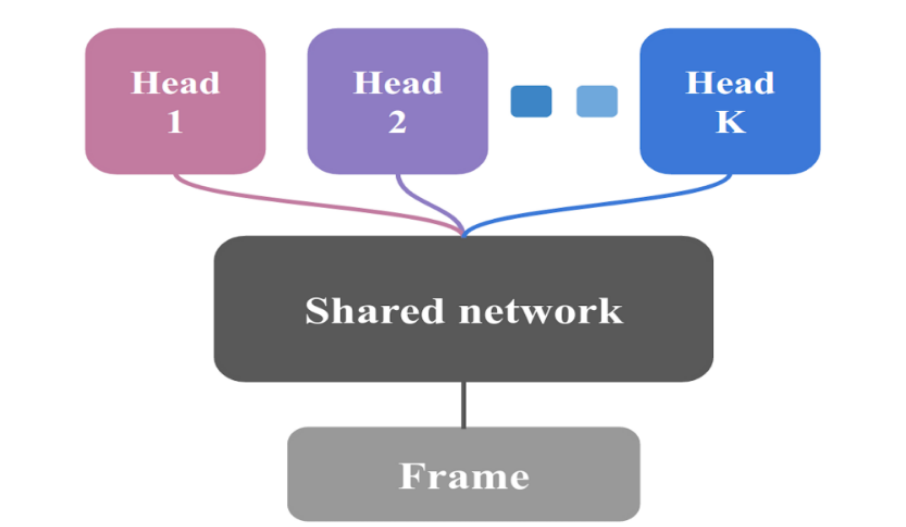
\includegraphics[width=\linewidth]{BDQN_Architecture.png}
 \caption{Network architecture in Bootstrapped DQN ~\cite{DBLP:journals/corr/OsbandBPR16}.}
 \label{fig:BDQN_Architecture}
\end{figure}
Bootstrapped DQN uses a parametrized estimate of the Q-value function, $Q(s,a;\theta)$, rather than a tabular encoding. A neural network is used to estimate this value, inspired from the architecture presented in ~\cite{mnih2015humanlevel}. The parameters $\theta$ are the weights of the neural network ~\cite{Goodfellow-et-al-2016}.\par
Bootstrapped DQN uses the modifications taken from DQN, to stabilize learning:
\begin{itemize}
\item The algorithm learns from sampled transitions from an experience buffer, rather than learning fully online,
\item The algorithm uses a target network with parameters $\theta^-$ that are copied from the learning network $\theta^- \leftarrow \theta_t$ only every $\tau$ time steps and then kept fixed in between updates.
\end{itemize}
The network update when executing action $a_t$ from state $s_t$, and observing reward $r_t$ and next state $s_{t+1}$ is :
\begin{equation}
\theta_{t+1} \leftarrow \theta_t +\alpha(y^Q_t-Q(s_t,a_t;\theta_t)) \nabla_{\theta} Q(s_t,a_t;\theta_t)),
\end{equation}
 where $\alpha$ is the learning rate and $y^Q_t$ is the target value. Bootstrapped DQN uses the target value of Double DQN ~\cite{Goodfellow-et-al-2016} to further stabilize learning. The target value $y^Q_t$ is as follows:
 \begin{equation}
 \label{eq:double_DQN_target}
 y^Q_t\leftarrow r_t+ \gamma \max_a Q(s_{t+1}, \argmax_{a} Q(s_{t+1},a;\theta_t);\theta^-).
 \end{equation}
 The Double DQN target is an elegant modification to stabilize learning. The update uses the main network to find the optimal action in the next state, but uses the value of this action from the target network. By doing this, we lower the positive bias introduced by the $\max$ operation in Q-Learning.\par
Bootstrapped DQN modifies DQN to approximate a distribution over Q-values via the bootstrap. At the start of each episode, bootstrapped DQN samples a single Q-value function from its approximate posterior. The agent then follows the policy which is optimal for that sample for the duration of the episode. The authors argue this is a natural adaptation of the Thompson sampling heuristic to RL that allows for temporally extended (or deep) exploration ~\cite{Strens00abayesian,NIPS2013_5185}. The algorithm can be implemented efficiently by building up $K \in \mathbb{N}$ bootstrapped estimates of the Q-value function in parallel as in Figure ~\ref{fig:BDQN_Architecture}. It is important to clarify that each one of these value function function heads $Q_k(s,a;\theta)$ is trained against its own target network $Q_k(s,a;\theta^-)$. This means that each $Q_1, \ldots, Q_K$ provide a temporally extended (and consistent) estimate of the value uncertainty via TD estimates. \par 
The algorithm also stores a mask, $w_1, \ldots, w_K \in \{0, 1\}$ indicating data are used to train which head. The mask, $m_t$, is a core idea of the full Bootstrapped DQN algorithm because it decides, for each value function $Q_k$, whether or not it should train upon the experience generated at step $t$. In its simplest form $m_t$ is a binary vector of length $K$, masking out or including each value function for training on that time step of experience (\ie should it receive gradients from the corresponding experience $(s_t, a_t, r_t, s_{t+1},m_t)$). The masking distribution $M$ is responsible for generating each $m_t$. For example, when $M$ yields $m_t$ whose components are independently drawn from a Bernoulli distribution with parameter 0.5 then this corresponds to the double-or-nothing bootstrap ~\cite{owen2012}. On the other hand, if $M$ yields a mask $m_t$ with all ones, then the algorithm reduces to an ensemble method.\par
Periodically, the replay buffer is played back to update the parameters of the value function network $Q$. The gradients of the $k$-th value function $Q_k$ for the $t$-th tuple in the replay buffer $B$, $g_t^k$ is:
\begin{equation}
g_t^k=m_t^k(y_t^Q-Q_k(s_t,a_t;\theta))\nabla_{\theta}Q(s_t,a_t;\theta),
\end{equation}
where $y_t^Q$ is the target value given by (~\ref{eq:double_DQN_target}). Pseudocode of the algorithm is shown in Alg.~\ref{alg:bootstrapped_dqn}.
\begin{algorithm}[H]
	\textbf{INPUT:} Value function networks $Q$ with $K$ outputs $\lbrace Q_k \rbrace_{k=1}^{K}$, Masking distribution $M$.
 \begin{algorithmic} 
 \State Let $B$ be a replay buffer storing experience
 \For{each episode}
 \State Obtain initial state $s_0$
 \State Pick a value function to act using $k \sim Uniform\lbrace1, \ldots, K\rbrace$
 \For{step $t=1, \ldots$ until end of episode}
 	\State Pick an action according to $a_t \in \argmax_a Q_k(s_t,a)$
 	\State Take action $a_t$, and observe $r_t,s_{t+1}$
 	\State Sample bootstrap mask $m_t \sim M$
 	\State Add experience ($s_t,a_t,r_t,s_{t+1},m_t)$ to replay buffer $B$
 \EndFor
 \EndFor
 \end{algorithmic}
	\caption{Bootstrapped DQN}
 \label{alg:bootstrapped_dqn}
\end{algorithm}

\section{Distributional RL} \label{distributional_rl}
In the previous chapter we reviewed the theory behind Distributional RL, and the essential importance of the value distribution. Although the distributional framework is not derived to guide exploration, it provides some relevant ideas we will reuse in our algorithm. We recall $Z(s,a)$ is the random variable denoting the total return collected by the agent starting from state $s$, executing action $a$ and then following an optimal policy, the expected value of which is $Q(s,a)$. In this section we will review two recent algorithms that belong to this class.
\subsection{Approximate Distributional Learning: C51}
In this section we discuss a recent algorithm based on the distributional Bellman optimality operator discussed in the previous chapter. C51 ~\cite{DBLP:journals/corr/BellemareDM17} models the value distribution using a discrete distribution parametrized by $N \in \mathbb{N}$ and $V_{MIN}, V_{MAX} \in \mathbb{R}$. The support of the distribution is given by a set of \emph{atoms} $\lbrace z_i= V_{MIN} + i\Delta z : 0 \leq i < N \rbrace, \Delta z= \frac{V_{MIN}-V_{MAX}}{N-1}$. The atom probabilities are given by a parametric model $\theta: \mathcal{S} \times \mathcal{A} \rightarrow R^N$. 
\begin{equation}
Z_{\theta}(s,a) =z_i \qquad w.p. 	\quad p_i(s,a)= \frac{e^{\theta_i(s,a)}}{\sum_{j=0}^{N-1}e^{\theta_j(s,a)}}.
\end{equation}
This discrete distribution is highly expressive and computationally friendly ~\cite{VanDenOord:2016:PRN:3045390.3045575}.\par
The algorithm works as follows:
\begin{itemize}
	\item From $(s,a)$, sample a transition, $r, S', A' \sim R(s,a), P(\cdot|s,a), \pi(\cdot|S')$, where $\pi$ the policy the agent follows;
	\item Compute the \emph{sample backup} given as:
	\begin{equation}
	\hat{\mathcal{T}}^\pi Z(s,a)=r+\gamma Z(S',A');
	\end{equation}
	\item Project this distribution onto the discrete distribution $z_\theta$, $\Phi \widehat{T}^\pi Z(s,a)$;
	\item Update towards projection, \ie take a KL-minimizing step.
\end{itemize}
\subsubsection{Projection step}
C51 reduces the Bellman update, discussed in the previous chapter, to multiclass classification by projecting the update $\hat{\mathcal{T}}z_\theta$ into the support of $z_{\theta}$. We recall the Bellman Operator defined in (~\ref{eq:bellman_distributional}). Figure ~\ref{fig:distributional_operator} gives an idea of this step. The framework is the same. The agent is at state $s$, executes action $a$, and observes reward $r$ and next state $s'$. We start from our prior belief about the distribution of the return in the next state, seen in Figure ~\ref{fig:distributional_operator} (a) in the figure. We want to learn from the experience collected. In Figure ~\ref{fig:distributional_operator} (b) we see how our distribution in the next state shrinks after we multiply it with the discount factor $\gamma$, and in Figure ~\ref{fig:distributional_operator} (c) we see the shifted distribution after adding the observed reward $r$. The projection step mentioned above can be seen in Figure ~\ref{fig:distributional_operator} (d). Discounting shrinks the distribution, so the target and the approximation have a disjoint support, and the KL divergence is infinite, so we cannot apply a minimization step. C51 solves this by taking every atom of the target distribution, and mapping them to its two nearest neighbors.\par
\begin{figure}
 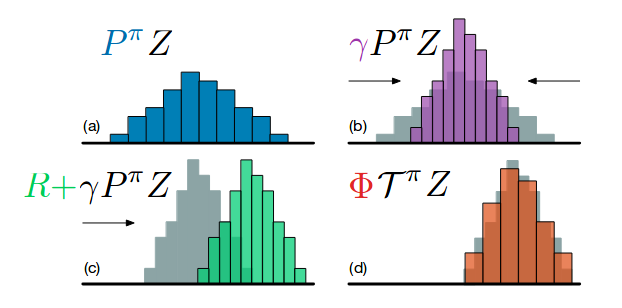
\includegraphics[width=\linewidth]{distributional_bellman_operator.png}
 \caption{Visualization of the distributional Bellman operator ~\cite{DBLP:journals/corr/BellemareDM17}.}
 \label{fig:distributional_operator}
\end{figure}
More formally, let $\pi$ be the greedy policy \wrt $\mathbb{E}[Z_\theta]$. Given a sample transition $(s,a,r,s′)$, we compute the Bellman update $\widehat{T}z_j=r+\gamma z_j$ for each atom $z_j$, then distribute its probability $p_j(s′,\pi(s′))$ to the immediate neighbours of $\widehat{T}z_j$. The $i$th component of the projected update $\Phi \widehat{T}^\pi Z(s,a)$ is:
\begin{equation}
	\Phi \widehat{T}^\pi Z(s,a)_i=\sum_{j=0}^{N-1} \left[1- \frac{\vert [\widehat{T}z_j]_{V_{MIN}}^{V_{MAX}} -z_i  \vert}{\Delta z} \right]_{0}^{1},
\end{equation}
where $[\quad]_{a}^{b}$ bounds its arguments in the range $[a,b]$. Pseudocode of the algorithm is shown in Alg. ~\ref{alg:c51}
\begin{algorithm}[H]
\begin{flushleft}
 \textbf{Input:} A transition $s_t,a_t,r_t,s_{t+1}$, $\gamma \in [0,1]$\\
 \textbf{Output:} Loss
\end{flushleft}
 \begin{algorithmic}
 \State $Q(s_{t+1},a)= \sum_{i} z_i p_i(s_{t+1},a)	\qquad \forall a$
 \State $a^* \leftarrow \argmax_a Q(s_{t+1},a)$
 \State $m_i=0, i \in 0, \cdots, N-1$
 \For{$j \in 0, \cdots, N-1$}
 		\State $\widehat{T}z_j \leftarrow [r+\gamma z_j]_{V_{MIN}}^{V_{MAX}}$
 		\State $b_j \leftarrow (\widehat{T}z_j- V_{MIN}) / \Delta z$
 		\State $l \leftarrow \lfloor b_j\rfloor, u \lceil b_j \rceil$
 		\State $m_l \leftarrow m_l+ p_j(s_{t+1},a^*)(u-b_j)$
 		\State $m_u \leftarrow m_u+ p_j(s_{t+1},a^*)(b_j-l)$
 \EndFor
 \Return $-\sum_{i} m_i \log p_i(s_t,a_t)$
 \end{algorithmic}
 \caption{$C51$ algorithm}
 \label{alg:c51}
\end{algorithm}
\subsection{Distributional Reinforcement Learning with Quantile Regression}
One of the theoretical contributions of the C51 work was a proof that the distributional Bellman operator is a contraction in a maximal form of the Wasserstein metric between probability distributions. 
Unfortunately, as noted by the authors, and further developed by Bellemare et al., the Wasserstein metric, viewed as a loss, cannot generally be minimized using stochastic gradient methods ~\cite{DBLP:journals/corr/BellemareDM17}. This negative result left open the question as to whether it is possible to devise an online distributional reinforcement learning algorithm which takes advantage of the contraction result of the Wasserstein metric. Instead, the C51 algorithm first performs a heuristic projection step, followed by the minimization of a KL divergence between projected Bellman update and prediction. C51 therefore leaves a theory-practice gap in our understanding of distributional reinforcement learning, which makes it difficult to explain the good performance of C51.\par
By appealing to the theory of \emph{quantile regression} ~\cite{koenker2005quantile}, Dabney et al. in ~\cite{DBLP:journals/corr/abs-1710-10044}, propose an algorithm, applicable in a stochastic approximation setting, which can perform distributional reinforcement learning over the Wasserstein metric. Recall that C51 approximates the distribution at each state-action pair by attaching variable (parametrized) probabilities $p_1,\ldots,p_N$ to fixed locations $z_1 \leq \ldots \leq z_N$. Quantile Regression DQN's approach is to ``transpose'' this parametrization by considering fixed probabilities but variable locations. Specifically, we take uniform weights, so that $p_i= \frac{1}{N}$ for each $i = 1,\cdots,N$. This new distribution aims to estimate \emph{quantiles} of the target distribution, hence the name \emph{quantile distribution}. Let $\mathcal{Z}_Q$ be the space of quantile distributions for a given $N$. We will denote the cumulative probabilities associated to such a distribution by $\tau_1, \ldots, \tau_N$, so that $\tau_i=\frac{i}{N}$ for $i=1, \ldots, N$.\par
Formally, let $\theta: \mathcal{S} \times \mathcal{A} \rightarrow R^N$ be some parametric model. A quantile distribution, $Z_\theta \in \mathcal{Z}_Q$ maps each state-action pair $(s,a)$ to a uniform probability distribution supported on $\lbrace \theta_i(s,a) \rbrace$. That is:
\begin{equation}
	\label{eq:quantile_distribution}
	Z_\theta(s,a)= \frac{1}{N} \sum_{i=1}^{N} \delta_{\theta_i(s,a)},
\end{equation} 
where $\delta_z$ denotes a \emph{Dirac} at $z \in \mathbb{R}$.\par
Compared to the parametrization of C51, the benefits of a parameterized quantile distribution are threefold. 
\begin{itemize}
\item We are not restricted to prespecified bounds on the support, or a uniform resolution, potentially leading to significantly more accurate predictions when the range of returns vary greatly across states;
\item This also lets us do away with the projection step present in C 51, as there are no issues of disjoint supports. This obviates the need for domain knowledge about the bounds of the return distribution when applying the algorithm to new tasks;
\item This reparametrization allows us to minimize the Wasserstein loss, without suffering from biased gradients, specifically, using quantile regression ~\cite{DBLP:journals/corr/abs-1710-10044}.
\end{itemize}
\subsubsection{The Quantile Approximation}
It is well-known that in reinforcement learning, the use of function approximation may result in instabilities in the learning process ~\cite{Tsitsiklis97ananalysis}. Specifically, the Bellman update projected onto the approximation space may no longer be a contraction. Dabney et al. analyze the distributional Bellman update, projected onto a parameterized quantile distribution, and prove that the combined operator is a contraction. \par
We are interested in quantifying the projection of an arbitrary value distribution $Z \in \mathcal{Z}$ onto $\mathcal{Z}_Q$, that is:
\begin{equation}
	\Pi_{d_1}Z= \argmin_{Z_\theta \in \mathcal{Z}_Q} d_1(Z,Z_\theta).
\end{equation}
Let $Y$ be a distribution with bounded first moment and $U$ be a uniform distribution over $N$ Diracs as in [~\ref{eq:quantile_distribution}] with support $\lbrace \theta_1, \ldots, \theta_N \rbrace$. Then the 1-Wasserstein distance is:
\begin{equation}
	d_1(Y,U)= \sum_{i=1}^{N} \int_{\tau_{i-1}}^{\tau_i} \vert F_Y^{-1}(\omega)- \theta_i \vert d \omega,
\end{equation}
where $F_Y^{1}$ is the quantile function of $Y$. We are looking for the parametrized distribution that minimizes this distance. Dabney et al. prove in ~\cite{DBLP:journals/corr/abs-1710-10044} the following: 
\begin{lemma}
	For any $\tau, \tau' \in [0,1]$ with $\tau < \tau'$ and cumulative distribution $F$ with inverse $F^{-1}$, the set of $\theta \in \mathbb{R}$ minimizing $\int_{\tau_{i-1}}^{\tau_i} \vert F_Y^{-1}(\omega)- \theta_i \vert d \omega$ is given by 
	\begin{equation*}
		\left\lbrace \theta \in \mathbb{R} \vert F(\theta)=\frac{\tau+\tau'}{2} \right\rbrace.
	\end{equation*}
	\label{lem:MinQuantileDist}
\end{lemma}
These \emph{quantile midpoints} will be denoted by $\hat{\tau}_i=\frac{\tau_{i-1}+\tau_i}{2}$ for $1 \leq i \leq N$. Therefore, by Lemma \ref{lem:MinQuantileDist}, the values for $\lbrace \theta_1,\theta_2,\ldots,\theta_N\rbrace$ that minimize $d_1(Y,U)$ are given by $\theta_i=F^{-1}_Y(\hat{\tau_i})$.\par
Dabney et al. prove that the combination of the projection implied by quantile regression with the Bellman operator is a contraction in $\infty$-Wasserstein metric, \ie the largest gap between the two c.d.fs. More formally, for any two value distributions $Z_1, Z_2 \in \mathcal{Z}$ for an MDP with countable state action spaces, 
\begin{equation}
\overline{d}_{\infty}(\Pi_{d_1} \mathcal{T}^\pi Z_1,\Pi_{d_1} \mathcal{T}^\pi Z_2) \leq \gamma \overline{d}_{\infty} (Z_1,Z_2),
\end{equation}
where $\Pi_{d_1} \mathcal{T}^\pi$ is the combined Bellman operator.\par
Following these results, Dabney et al. use the \emph{quantile regression loss}, which is an asymmetric convex loss that penalizes overestimation errors with weight $\tau$ and underestimation errors with weight $1-\tau$. More formally, for a distribution $Z$, and a given quantile $\tau$, the value of the quantile function $F_Z^{-1}(\tau)$ may be characterized as the minimizer of the quantile regression loss:
\begin{equation}
\begin{split}
\mathcal{L}_{QR}^{\tau}(\theta) & =\mathbb{E}_{\hat{Z} \sim Z}[\rho_{\tau}(\hat{Z}-\theta)], \text{where} \\
\rho_{\tau}(u) & = u(\tau- \delta_{\lbrace u<0 \rbrace}) \quad \forall u \in \mathbb{R}.
\end{split}
\label{eq:quantile_regression_loss}
\end{equation} 
More generally, we have that the minimizing values of $\lbrace \theta_1,\theta_2,\ldots,\theta_N\rbrace$ for $d_1(Z,Z_\theta)$ are those that minimize the following objective
\begin{equation*}
	\sum_{i=1}^{N} =\mathbb{E}_{\hat{Z} \sim Z}[\rho_{\tau}(\hat{Z}-\theta_i)].
\end{equation*}
This loss gives unbiased sample gradients. As a result, we can find the minimizing $\lbrace \theta_1,\theta_2,\ldots,\theta_N\rbrace$ by stochastic gradient descent. In practice the authors use the \emph{quantile Huber loss}, the asymmetric variant of the Huber loss ~\cite{huber:1964}, given by:
\begin{equation}
\mathcal{L}_k(u)=
		\begin{cases}
 \frac{1}{2}u^2 &\quad\text{if }\vert u \vert \leq k\\
 k(\vert u \vert - \frac{1}{2} k) &\quad\text{otherwise}. \\
 \end{cases}
\end{equation}
The Quantile huber loss is simply:
\begin{equation}
	\rho^k_\tau (u)=\vert \tau - \delta{\lbrace u<0 \rbrace} \vert \mathcal{L}_k(u).
\label{eq:quantile_huber_loss}
\end{equation}
\subsubsection{QRTD}
Recall the standard TD update from Chapter 1. TD allows us to update the estimated value function with a single unbiased sample following $\pi$. Quantile regression also allows us to improve the estimate of the quantile function for some target distribution, $Y(s)$, by observing samples $y \sim Y(s)$ and minimizing Equation (~\ref{eq:quantile_regression_loss}). Using these results, Dabney et al. in ~\cite{DBLP:journals/corr/abs-1710-10044} define the quantile regression temporal difference (QRTD) learning algorithm summarized by the update: 
\begin{equation}
\theta_i(s) \leftarrow \theta_i(s)+ \alpha(\hat{\tau}_1- \delta_{\lbrace r+\gamma z' < \theta_i(s) \rbrace}),
\end{equation}
where $Z_\theta$ is a quantile distribution as in (~\ref{eq:quantile_distribution}) and $\theta_i(s)$ is the estimated value of $F^{-1}_{Z^{\pi}(s)}(\hat{\tau}_i)$ in state $s$. It is important to note that this update is for each value of $\hat{\tau}_i$ and is defined for a single sample from the next state value distribution. In general it is better to draw many samples of $z′\sim Z(s′)$ and minimize the expected update. Another approach, used by the authors, is to compute the update for all pairs of $(\theta_i(s),\theta_j(s′))$.
\subsubsection{Quantile Regression DQN}
Quantile Regression DQN builds from the DQN architecture described in ~\cite{mnih2015humanlevel}. The algorithm requires two modifications to DQN. First, it uses a nearly identical neural network architecture as DQN, only changing the output layer to be of size $\vert A \vert \times N$, where $N$ is a hyper-parameter giving the number of quantile targets. Second, it replaces the Huber loss used by DQN,  with the quantile Huber loss given in Equation (~\ref{eq:quantile_huber_loss}). Pseudocode of the algorithm is given in Alg. ~\ref{alg:QRDQN}.
\begin{algorithm}[H]
\begin{flushleft}
 \textbf{Input:} A transition $s,a,r,s'$, $\gamma \in [0,1]$\\
 \textbf{Output:} Quantile Regression Loss
\end{flushleft}
 \begin{algorithmic}
 \State $Q(s',a')= \sum_{j} q_j \theta_j(s',a')	\qquad \forall a$
 \State $a^* \leftarrow \argmax_a Q(s',a)$
 \State $\mathcal{T}\theta_j \leftarrow r+ \gamma \theta_j(s',a^*), \quad \forall j$
 \State \Return $\sum_{i=1}^{N} \mathbb{E} \left[ \rho^k_{\hat{\tau}_i}(\mathcal{T}\theta_j - \theta_i(s,a)) \right]$
 \end{algorithmic}
 \caption{$QR-DQN$ algorithm}
 \label{alg:QRDQN}
\end{algorithm} 
\chapter{Particle Q Learning} \label{chap:chapter4}
The exploration vs. exploitation dilemma is still an open problem in RL. Classic exploration approaches like $\epsilon$-greedy or Boltzman work well for simple problems, but they do not address temporally extended (or deep) exploration. In Chapter 2 we discussed some classic and modern, model-free and model-based algorithms that do efficient or deep exploration. In this chapter we propose a new model-free approach to the exploration vs. exploitation tradeoff. \emph{Particle Q Learning} explicitly expresses the uncertainty about the Q-value estimates by maintaining Q-value distributions and uses them to make better decisions during the learning process. We approximate the Q-value distribution by attaching fixed weights to variable (parametrized) locations. We call these parametrized locations, \emph{particles}, hence the name. This way we attempt to estimate the quantiles of the target distribution. \par
We begin in Section ~\ref{sec:q_value_distributions} where we define our approximation of the Q-distribution and derive some interesting results. In Section ~\ref{sec:action_selection} we propose two possible policies that use the Q-distributions as defined in Section ~\ref{sec:q_value_distributions}. Finally, in Section ~\ref{sec:updating_q_distributions},  we discuss how to maintain the distributions from samples of experience $(s,a,r,s')$.

\section{Q Value Distributions} \label{sec:q_value_distributions}
A reinforcement learning agent needs to do exploration because he is uncertain about the true Q-values of the actions. Indeed, this uncertainty is the reason for doing learning in the first place. An agent that is certain about the Q-value estimates of all the action has no reason to explore, since it does not expect there to be a better policy to discover. It seams reasonable to us, that decisions whether to explore new actions or to exploit the current best ones, should be done based on how uncertain the agent is about the Q-values. Therefore this uncertainty should be expressed explicitly in an RL agent.\par
We represent the uncertainty we have about the Q-value estimates, using a \emph{Q-distribution}, a probability distribution over the possible values that the Q-value might take. Formally, let $R_{s,a}$ be a random variable that denotes the total discounted reward received when action $a$ is executed in state $s$ and then an optimal policy is followed. We note that $Q^*(s,a)=\mathbb{E}[R_{s,a}]$. The objective of the agent is to learn $\mathbb{E}[R_{s,a}]$, and not approximate the whole distribution of $R_{s,a}$, as the knowledge of the expectation of the return is sufficient to act optimally. In this section we will review the proposed Q-value distribution.
\subsection{Particle Q Distribution}
We will denote with $Q(s,a)$ the random variable representing the expected cumulative reward from $(s,a)$ following the optimal policy. To approximate this distribution we will use a parametric model, parametrized over $N$ locations, which we call particles, associated to fixed weights $\frac{1}{N}$. We indicate with $\mathcal{Q}(s,a)$ the set of particles associated to $(s,a)$ ($\vert \mathcal{Q}(s,a) \vert =N$):
\begin{equation}
\mathcal{Q}(s,a)={x^i_{s,a} \qquad i=1, \ldots,N}.
\end{equation}
where $x^i_{s,a}$, is the $i$th particle of the state action pair $(s,a)$. We will assume, without loss of generality, $x_1 \leq x_2 \ldots \leq x_N$. This way, the Q-distribution is approximated by the following \emph{mixture of deltas}:
\begin{equation}
	p(x \vert s,a)=\sum_{i=1}^{N} \frac{1}{N} \delta(x-x^i_{s,a}).
	\label{eq:particle_distribution}
\end{equation}
The c.d.f is given by:
\begin{equation}
\hat{F}(x \vert s,a) = \sum_{i=1}^{N} \frac{1}{N} H(x-x^i_{s,a}),
\end{equation}
where H is the Heaviside step function, defined as:
\begin{equation}
	H(x) = \begin{cases}
    			1 & x \ge 0 \\
                0 & x < 0
    		\end{cases}.
\end{equation}
Using this parametrized distribution, we try to estimate the quantiles of the Q-distribution.\par
It is important to note the fundamental difference between maintaining a distribution of the return $R_{s,a}$, and the distribution of the Q-values, $\mathbb{E}[R_{s,a}]$. While the return $R_{s,a}$ has an intrinsic randomness, which might come from different factors  like the stochasticity of the underlying model of the MDP or the randomness of the reward function, the Q-values are the expected value of this return. We keep a distribution of the Q-values to represent our uncertainty about the current estimate. We expect that at the end of the learning process this distribution shrinks to the real Q-value. On the other hand, when maintaining the distribution of the return, the distribution will remain wide to represent the intrinsic randomness of the MDP. Figure ~\ref{fig:q_distribution_behaviour} shows the expected behavior of the learning process. The distribution will start flat (given that the prior is initialized that way). As the learning process continues, the agent observes a sequence of values from $\mathbb{E}[R_{s,a}]$ and updates its belief. As the learning process continues, the distribution should get progressively more peaked and the agent becomes more certain about the actual Q-value.
\begin{figure}
 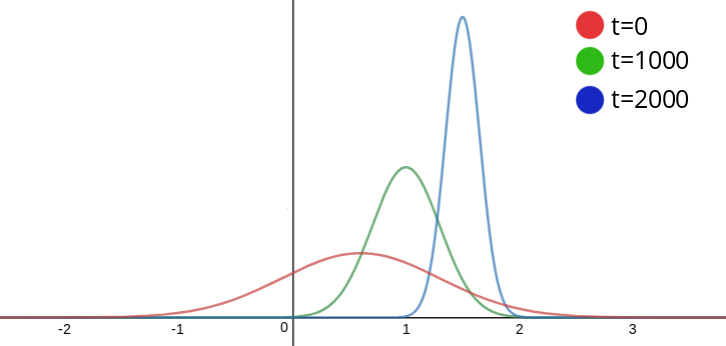
\includegraphics[width=\linewidth]{q_distribution_behaviour.jpg}
 \caption{Behaviour of the Q-distribution over time.}
 \label{fig:q_distribution_behaviour}
\end{figure}
\subsection{Sample Mean Distribution}
We consider a collection of random variables $\{X_i\}_{i=1}^m$ and $I \in \{1,\dots,m\}$ a random index; we aim to estimate the mean $\widehat{\mu}_Y$ of $Y = X_{I}$ assuming to have estimations of the means $\widehat{\mu}_{X_i}$ of $X_i$. We assume $I \sim \rho$ where $\Pr(I = i) = \xi_i$ unknown. Standard Monte Carlo estimation would sample $I$ from $\rho$ distribution $N$ times and perform the estimate:
\begin{equation}
	\widehat{\mu}_{Y}^{MC} = \frac{1}{N} \sum_{j=1}^N \widehat{\mu}_{X_{I_j}}, \quad I_j \sim \rho.
\end{equation}
Suppose to know the distribution of the sample means $\widehat{\mu}_{X_i} \sim \nu_i$. Which is the best approximating distribution for the sample mean? In~\cite{NIPS2017_7149}, in the context of Gaussian processes, the authors claim that by tacking the convolution of the single distributions $\nu_i$ properly weighted with $\xi_i$ would underestimate the uncertainty on $\widehat{\mu}_{Y}^{MC}$. Indeed, if $m\rightarrow \infty$ the uncertainty would be null. Contrary, we could find the distribution $\nu$ minimizing:
\begin{equation}
	\mathcal{L}_d^p (\nu) = \mathbb{E}_{I \sim \rho} \left[ d(\nu, \nu_I)^p \right],
\end{equation}
where $d$ is a suitable distribution divergence and $p>0$. $\nu^* = \argmin_{\nu \in \mathcal{N}} \mathcal{L}_d^p (\nu)$ is called \emph{Barycenter}~\cite{journals/siamma/AguehC11} of $\{\nu_i\}_{i=1}^m$ \wrt divergence $d$. The same loss function can be computed from samples as:
\begin{equation}
	\widehat{\mathcal{L}}_d^p (\nu)  = \frac{1}{N} \sum_{j=1}^N d(\nu, {\nu_{I_j}}), \quad I_j \sim \rho.
\end{equation}
If $\nu = \nu_{\theta}$ belongs to $\mathcal{N}_{\Theta} = \{ \nu_{\theta}: \theta \in \Theta \subseteq \mathbb{R}^d \}$ a parametrized distribution space differentiable in $\theta$ and $d$ is differentiable \wrt the first argument we can find the parameter $\theta^*$ via stochastic gradient descent:
\begin{equation}
	\theta^{(t+1)} = \theta^{(t)} - \alpha \nabla_\nu d(\nu, {\nu_{I}}) \nabla_{\theta} \nu_{\theta^{(t)}}, \quad I \sim \rho.
\end{equation}
\subsection{Approximation of a distribution function with mixture of delta functions}
We consider a c.d.f. $F(x)$ that we want to approximate with:
\begin{equation}
	\widehat{F}_n(x) = \frac{1}{n} \sum_{j=1}^n w_j H(x-x_j).
\end{equation}
We start considering the case in which $w_j$ are fixed.
We need to determine $x_j$ such that the distance between the distribution of $F(x)$ and $\widehat{F}_n(x)$ is minimal.Clearly, using discontinuous distributions the classical divergences like KL or TV are inappropriate (they are always maximal). We resort to the Wasserstein metric. We use $W_2(F, \widehat{F}_n)$ as metric.

\begin{theorem}
	Let $F(x)$ a c.d.f. of r.v. $X$ s.t. $X \in [a,b]$ a.s.. Then, the 2-Wasserstein distance $W_2(F, \widehat{F}_n)$ has the unique minimizer:
    \begin{equation}
    	\widehat{x}_j = \frac{1}{|I_j|} \int_{I_j} F^{-1}(t) \mathrm{d} t, \quad j=1,2,\dots, n,
    \end{equation}
    where $I_j=[t_{j-1}, t_j)$, $t_0 = 0$ and $t_j = \sum_{k=1}^j w_j$. In this case, the 2-Wasserstain distance can be bounded as:
    \begin{equation}
    	W_2(F, \widehat{F}_n) \le \frac{(b-a)^2}{4} \max_{j=1,2,\dots,n} |I_j|.
    \end{equation}
\end{theorem}

\begin{proof}
	Let us first compute the quantile function $\widehat{F}_n^{-1}$:
    \begin{equation}
    	\widehat{F}_n^{-1}(t) = \sum_{j=1}^n x_j \mathds{1}_{I_j}(t),
    \end{equation}
    where $\mathds{1}$ is the indicator function. The 2-Wasserstin distance can be written as:
    \begin{align*}
    	W_2^2(F, \widehat{F}_n) & = \int_0^1 \left( F^{-1}(x) - F_n^{-1}(x) \right)^2 \mathrm{d} t = \\
        & = \sum_{j=1}^n \int_{I_j} \left( F^{-1}(x) - x_j \right)^2  \mathrm{d} t. 
    \end{align*}
    We take the derivative \wrt $x_j$ and we get:
    \begin{equation}
    	\frac{\partial W_2^2}{\partial x_j} = -2 \int_{I_j} \left( F^{-1}(x) - x_j \right)  \mathrm{d} t = 0.
    \end{equation}
    From which the first result follows. Let us now observe, since $F^{-1}$ is monotonically increasing, that for every $j$:
    \begin{align*}
    	\int_{I_j} \left(F^{-1}(x) - \widehat{x}_j\right)^2 \mathrm{d} t & \le \int_{I_j} \left(F^{-1}(x) - \frac{F^{-1}(t_j) - F^{-1}(t_{j-1}) }{2}\right)^2 \mathrm{d} t \le \\
        & \le\frac{1}{4} \int_{I_j} \left( (F^{-1}(x) - F^{-1}(t_j)) +  (F^{-1}(x) - F^{-1}(t_{j-1})) \right)^2 \mathrm{d} t \le \\
        & \le \frac{1}{4} \int_{I_j} \left( (F^{-1}(x) - F^{-1}(t_j)) -  (F^{-1}(x) - F^{-1}(t_{j-1})) \right)^2 \mathrm{d} t \le \\
       & \le\frac{1}{4} \int_{I_j} \left( F^{-1}(t_j) - F^{-1}(t_{j-1} \right)^2 \mathrm{d} t \le \\
       & \le \frac{1}{4} |I_j| \left( F^{-1}(t_j) - F^{-1}(t_{j-1}) \right)^2.
    \end{align*}
    Let us call $\Delta_j = F^{-1}(t_j) - F^{-1}(t_{j-1})$, the error can be bounded overall as:
    \begin{align*}
    	W_2^2(F, \widehat{F}_n) & \le \frac{1}{4}  \sum_{j=1}^n |I_j| \Delta_j ^2 \le \\
        & \le \frac{1}{4} \max_j |I_j| \sum_{j=1}^n \Delta_j ^2 \le \\
        & \le \frac{1}{4} \max_j |I_j| \left( \sum_{j=1}^n \Delta_j \right) ^2 \le \\
        & \le \frac{1}{4} \max_j |I_j| \left(b-a\right) ^2,
    \end{align*}
    where we used Cauchy–Schwarz inequality ~\cite{Steele:2004:CMC:993490} in the last passage, observing that $\Delta_j \ge 0$ from the monotonicity of $F^{-1}$.
\end{proof}

For the case of uniform $w_j = 1/n$ the result reduces to:
\begin{equation}
	W_2^2(F, \widehat{F}_n) \le \frac{(b-a)^2}{4N}.
\end{equation}
Thus if $N\rightarrow \infty$ the error goes to zero. Up to now we considered the error introduced by representing a given distribution with a mixture of deltas. 

It is interesting to investigate the properties of the approximating distribution $\widehat{F}_n$

\begin{prop}
	Let $\widehat{F}_n$ be the approximating c.d.f. of $F$ as defined before. Then it holds that:
    \begin{equation}
    	\ev_{\widehat{F}_n} [X] = \ev_{F} [X].
    \end{equation}
\end{prop}

\begin{proof}
	We first observe that by making the substitution $x = F^{-1}(t)$ we have the identity:
    \begin{equation}
    	\int_{I_j} F^{-1}(t) \mathrm{d} t = \int_{F^{-1}(t_{j-1})}^{F^{-1}(t_{j})} x f(x) \mathrm{d}x.
    \end{equation}
    Therefore:
    \begin{align*}
    	\ev_{\widehat{F}_n} [X] & =\int_a^b x \widehat{f}_n(x) \mathrm{d}x = \\
        & = \sum_{j=1}^n w_j x_j = \\
        & = \sum_{j=1}^n w_j \frac{1}{|I_j|} \int_{I_j} F^{-1}(t) \mathrm{d} t = \\
        & = \sum_{j=1}^n \int_{I_j} F^{-1}(t) \mathrm{d} t = \\
        & = \sum_{j=1}^n \int_{F^{-1}(t_{j-1})}^{F^{-1}(t_{j})} x f(x) \mathrm{d}x = \\
        & = \int_{a}^{b} x f(x) \mathrm{d}x = \ev_{F} [X].
    \end{align*}
\end{proof}

Thus, our approximation preserves the mean. This does not hold in general for the other moments.


Now we move to the problem of finding a proper Wasserstein barycenter.
\subsection{Wasserstein barycenter} 
We represent the distribution of the sample mean by means of uniform ($w_j=1/n$) mixtures of Dirac deltas. Our problem is to determine the 2-Wasserstein barycenter of a set of mixtures differently weighed with the same number of components. 
\begin{equation}
\label{eq:problem}
	\widehat{\mathbr{x}} = \argmin_{\mathbr{x}} \sum_{i=1}^m \xi_i W_2^2(F_X, F_{Y_i}),
\end{equation}
where $f_X(x) = 1/n \sum_{j=1}^n \delta(x-x_j)$ and $f_{Y_i}(x) = 1/n \sum_{j=1}^n \delta(x-y_{ij})$. We will prove that this problem has a closed form solution (remember that we assume to consider the $x$ and $y$ sorted):

\begin{theorem}
	The unique solution of the problem~\ref{eq:problem} is given by:
    \begin{equation}
    	\widehat{\mathbr{x}} = \mathbr{Y} \mathbr{\xi},
    \end{equation}
    where $\mathbr{Y} = (\mathbr{y}_1 | \dots | \mathbr{y}_m)$.
\end{theorem}

\begin{proof}
	We observe that, since all weights are $w_j = 1/n$, the relevant quantiles are the same for all involved distributions, \ie $1/n$. As a consequence, fixing $i$, we can easily compute the 2-Wasserstein distance as:
    \begin{equation}
    	W_2^2 (F_X, F_{Y_i}) = \frac{1}{n} \sum_{j=1}^n (x_j - y_{ij})^2 = \frac{1}{n} \| \mathbr{x} - \mathbr{y}_i \|^2_2.
    \end{equation}
    Thus, the objective function can be written as:
    \begin{equation}
    	\mathcal{L}(\mathbr{x}) = \frac{1}{n} \sum_{i=1}^m \xi_i \| \mathbr{x} - \mathbr{y}_i \|^2_2.
    \end{equation}
    This is a convex function, all it takes is to vanish the gradient:
    \begin{equation}
    	\nabla_{\mathbr{x}} \mathcal{L}(\mathbr{x}) = \frac{2}{n} \sum_{i=1}^m \xi_i (\mathbr{x} - \mathbr{y}_i) = 0 \implies \mathbr{x} =  \sum_{i=1}^m \xi_i \mathbr{y}_i = \mathbr{Y} \mathbr{\xi},
    \end{equation}
    where $\mathbr{Y} = (\mathbr{y}_1 | \dots | \mathbr{y}_m)$.
\end{proof}

Clearly, in reality the probabilities $\xi_i$ are not known and we want to avoid to estimate them separately (this would bring to a model-based approach as the $\xi_i$ are the probabilities defining the transition model). For this purpose we look at the objective function as an expected value:
\begin{equation}
	 \mathcal{L}(\mathbr{x}) = \ev_{I \sim \rho} [W_2^2(F_X, F_{Y_I})] = \frac{1}{n} \sum_{j=1}^n \ev_{I \sim \rho} [(x_j - y_{Ij})^2].
\end{equation}
Therefore we can employ a SGD update rule for the $x_j$.
\begin{equation}
	\mathbr{x}^{(t+1)} = \mathbr{x}^{(t)} - \alpha \nabla_{\mathbr{x}} \widehat{\mathcal{L}}(\mathbr{x}^{(t)} ) =  \mathbr{x}^{(t)} - \frac{2\alpha}{n} (\mathbr{x}^{(t)} -\mathbr{y}_{i^{(t)}} )
\end{equation}

It is simple to prove that the Wasserstein barycenter satisfies the following relation:
\begin{equation}
	\ev_{F_X}[X] = \ev_{I \sim \rho} \ev_{F_{Y_I}} [Y_I].
\end{equation}

\section{Action Selection} \label{sec:action_selection}
The classical approach to exploration, applied in $\epsilon$-greedy or Boltzman exploration, is selecting actions with the highest Q-value estimate or randomly selecting an action based on the number of timesteps of learning performed. The heuristics of this is that, at the beginning of the learning process, the Q-value estimates are unreliable and exploration is done randomly. An exploration schedule is defined, based on the timesteps, so that as the learning progresses, exploration is done less and less, until it reaches 0 and the agent exploits the Q-values it has learned. This is done because there is no measure of the uncertainty of the Q-value estimates. \par 
In this section we will discuss two methods of choosing action based on the uncertainty of the Q-value estimates. The first one is an adaptation of Myopic VPI, used in ~\cite{Dearden98bayesianq-learning}. The idea is that, by using the Q-distributions, the agent can answer the exploration vs. exploitation dilemma explicitly, by weighting the benefits of exploiting the current best actions, versus the benefits of exploring new actions that give more information on the task at hand. In the limit, when the Q-distributions shrink to the true Q-values, Myopic VPI turns in a simple greedy policy that chooses the best actions. The second method, \emph{Weighted Policy}, choses actions based on the probability of each action of being maximal. Since we maintain distributions over Q-values, we can explicitly calculate the probabilities of each action to be optimal, and then execute the action with the highest probability.
\subsection{VPI Policy}
When the agent selects an action, we would like to strike a balance between present performance, the current optimal action based on our estimates, and future performance, actions that might turn out to be optimal in the future. This is in fact the essence of the exploration vs. exploitation dilemma. In our proposed approach, the agent maintains a Q-distribution for each state-action pair, $(s,a)$. Using these distributions, we can calculate the value of perfect information (VPI) ~\cite{4082064,Russell:1991:RTS:110787}, as in ~\cite{Dearden98bayesianq-learning}. This information is used to calculate the \emph{value of exploration}, hence balancing present and future performance.\par
As an example, consider Figure ~\ref{fig:q_distributions}. The Q-distributions of 3 different actions are shown. Choosing actions based on the mean of each distribution would result in a simple greedy policy, since the mean of the distribution is our estimate of $\mathbb{E}[R_{s,a}]$. Obviously action 1 is a bad choice. The distribution is pretty confident about the low return of this action, so the action is well explored. Consequently the likelihood of action 1 to be optimal is low, so by executing it we  will (very likely) lose in current performance and also will not learn any valuable information. Considering the means of the distributions action 3 is the current optimal action. Also the variance of its distribution is low, so we are confident of it's high return. Action 2 on the other had is certainly a candidate to be executed. The current cost of executing action 2, instead of the current optimal, is low, since the means of the two distributions are close. The second Q-distribution also has a high variance, which means we have low confidence on its real return, and exploring this action might actually be beneficial in the future. VPI measures the value of each action based on these kind of considerations.
\begin{figure}
 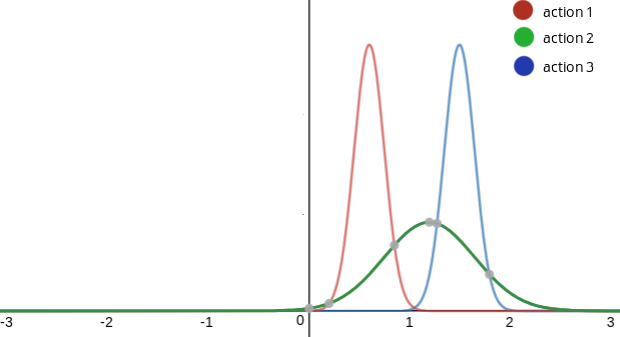
\includegraphics[width=\linewidth]{q_distributions.jpg}
 \caption{Q-distributions of 3 different actions.}
 \label{fig:q_distributions}
\end{figure}
To select which action to execute, the VPI is computed for each possible action in the current state. However, we have to consider also the cost of executing action $a$ instead of action $a_1$, the current optimal action. To select the action we have to consider the value VPI minus the difference in the expected value of $a$ and $a_1$. Formally, we choose the action that maximizes:
\begin{equation}
	VPI(s,a)- (\max_{a'} \mathbb{E}[Q(s,a')]- \mathbb{E}[Q(s,a)]).
\end{equation} 
Clearly, the expected value of the optimal action, $\max_{a'} \mathbb{E}[Q(s,a')$, is equal for all actions, so this strategy is equal to maximizing:
\begin{equation}
	VPI(s,a)+ \mathbb{E}[Q(s,a)].
\end{equation}
This way, the gain due to possible future observation is balanced with the cost of executing a current suboptimal action, instead of the current best one.\par
Computing the VPI can be thought as answering the question ``what would I be willing to pay to learn the true value, $v^*$, of this action''. If the information is worth a lot, then the information might be worth discovering through exploration. On the other hand, if the information is not worth a lot, it might be better to exploit the current optimal action. Let $q^*_{s,a}$ be the true expected value of action $a$ in state $s$. We first note that knowing the true value of the action is worth nothing is the current policy does not change ($VPI(s,a)=0$). Let $a_1$ be the current optimal action (\ie the action with the highest expected Q-value given the current information). Let $a_2$ be the action we currently believe is second best. If we learn that the true expected value of $a_1$ is higher than the expected value $a_1$, we have confirmed the current optimal policy, so we did not gain any new information. Note that the \emph{expectation} of the total discounted reward might have changed if we learned a new value for $a_1$, but the $actual$ expected discounted future reward is unchanged if we did not change our policy.  Similarly, if we learn the true value of some other action $a$, and we learn that the true value is still lower than the value of $a_1$, the new information has no value. \par 
We are left with two cases in which learning the true value of an action has some worth:
\begin{itemize}
\item When the new information shows that an action previously thought optimal is actually inferior to other actions,
\item When the new information shows that an action previously thought sub-optimal, is actually the optimal action.
\end{itemize} 
More formally, let $s$ be the current state, $a$ the action whose VPI is being calculated and $q_{s,a}$ a possible value of $Q^*(s,a)=\mathbb{E}[R_{s,a}]$. Let the two current best actions be $a_1$ and $a_2$. Then we can define the gain from learning that $a$ has expected value $q^*_{s,a}$ is ~\cite{Dearden98bayesianq-learning}:
\begin{equation}
	Gain_{s,a}(q^*_{s,a}) = \begin{cases}
    			\mathbb{E}[q_{s,a_2}]- q^*_{s,a}  & \text{if } a=a_1 \text{ and } q^*_{s,a}< \mathbb{E}[q_{s,a_2}] \\
                q^*_{s,a} - \mathbb{E}[q_{s,a_1}]  & \text{if } a \neq a_1 \text{ and  }q^*_{s,a}> \mathbb{E} [q_{s,a_1}] \\
                0 & \text{otherwise}
    		\end{cases}.
\end{equation}
Of course we do not have the value of $q^*_{s,a}$. Instead we have a Q-distribution over the value of $q^*_{s,a}$. So we can weight the gain of learning the true value of action $a$, $q^*_{s,a}$, with the probability of it being the true value according to the current Q-distribution, calculating the expected value of perfect information (EVPI) ~\cite{Dearden98bayesianq-learning} :
\begin{equation}
VPI(s,a)=\int_{-\infty}^{\infty} Gain_{s,a}(x) Pr(q_{s,a}=x) dx.
\label{eq:vpi_equation}
\end{equation}
In our case the Q-distriution is approximated using the particle distribution defined in (~\ref{eq:particle_distribution}). The integral in (~\ref{eq:vpi_equation}) turns into a sum over the particles as follows:
\begin{equation}
	VPI(s,a) = \begin{cases}
    			\sum_{x^k_{s,a} \leq \mathbb{E}[Q(s,a_2)]} \frac{1}{N}\left(\mathbb{E}[Q(s,a_2)]- x^k_{s,a}\right)  & \text{if } a=a_1 \\
                \sum_{x^k_{s,a} \geq \mathbb{E}[Q(s,a_1)]} \frac{1}{N}\left(x^k -\mathbb{E}[Q(s,a_1)]\right)  & \text{if } a \neq a_1 \\
    		\end{cases}.
\end{equation}
The value of perfect information estimate is used an a way of boosting the desirability of different actions. When the agent is confident about the value Q-value estimates VPI will go to zero and the VPI policy will turn to a simple greedy policy.
\subsection{Weighted Policy}
VPI policy tries to estimate the value of exploring a sub-optimal action, rather than exploiting the current best action. As Dearden et al. note in ~\cite{Dearden98bayesianq-learning}, this value of VPI is an optimistic assessment of the value of performing $a$. By executing $a$ we do not get perfect information about it's value, we just get one more training instance. We will now propose another policy that uses the Q-distributions maintained by our agent. \emph{Weighted policy} choses actions based on their probability of being optimal. Assuming that the Q-values of the different actions in state $s$ are independent (assumption that hardly holds in practice), the probability of  action $a$ to be optimal, $P(a= \argmax_{a'} Q(s,a'))$, is given by:
\begin{equation}
	\begin{split}
	P\left(a= \argmax_{a'} Q(s,a')\right) & = P\left(\forall a' \neq a, \prod Q(s,a) > Q(s,a')\right) \\
							   & = \int_{-\infty}^{\infty} P\left(Q(s,a)=x\right) \Pi_{a' \neq a} F_{a'}(x)dx
	\end{split},
	\label{eq:maximum_probability}
\end{equation}
where $F_{a'}(x)$ is the c.d.f. of the Q-distribution of action $a'$. Replacing the probabilities in (~\ref{eq:maximum_probability}), with our mixture of deltas distribution we get the following:
\begin{equation}
	P\left(a= \argmax_{a'} Q(s,a')\right)=\sum_{i=1}^{N} \frac{1}{N} \prod_{a' \neq a} \sum_{x_{a'}^j < x_a^i} \frac{1}{N}.
\end{equation}
Deriving the above formula is straightforward. The integral turns into a sum over the particles, for which $P(Q(s,a)=x^i_{s,a})=\frac{1}{N}$. 
\section{Updating the Q-distribution} \label{sec:updating_q_distributions}
In this section we will discuss how to update the Q-distributions maintained by the agent after executing a transition. We recall the agent maintains a distribution over Q-values , for each state-action pair, $(s,a)$, represented by a set of $N$ uniformly weighted particles. The problem at hand is how to move the set of particles $\mathcal{Q}(s,a)$ after observing local reward $r$. An obvious problem is that the distributions are over the Q-values whereas the agent observes samples from local reward, $R(s,a)$.
\par Suppose the agent is in state $s$, executes action $a$, and observes reward $r$ and next state $s'$. Let $R_{s'}$ be a random variable denoting the total sum of discounted reward from state $s'$ under an optimal policy. In this section we will see two methods to approximate the target distribution $R_{s'}$ and how to use to update the distribution of $Q(s,a)$.
\subsection{Sorted Update}
Suppose, after observing the transition $s,a,r,s'$, we have a set of $N$ particles , $\mathcal{Q}(s',a')$ representing our target distribution. The problem at hand is how to update the distribution of $Q(s,a)$ using this set of particles. The simplest idea would be to just add the new set of particles to the old set, building the set $\mathcal{Q}_{all}= \mathcal{Q}_{s,a} \cup \mathcal{Q}(s',a')$. The obvious problem with this approach is that the set would grow infinitely. We need to find the set of particles $\mathcal{Q}(s,a)$ that minimizes some sort of distance between the distribution represented from the set $\mathcal{Q}_{all}$. \par 
More formally, let $\mathcal{Q}^t(s,a)=x^t_i, \quad i=1,\ldots,N$ , $\mathcal{Q}'^t(s,a)=x'^t_i, \quad i=1,\ldots,N$ be the set of particles representing the prior and target distributions at step $t$. The set of particles minimizing the $W_2$ distance between the posterior and target distributions is given by:
\begin{equation}
	\label{eq:sorted_update}
	x^{t+1}_i \leftarrow x^{t}_i + \alpha (x'^{t}_i - x^{t}_i) \qquad i=1,\ldots,N , 
\end{equation}
where $\alpha$ is the learning rate. We recall that the set of particles are sorted. 
\subsection{Maximum Mean Updating}
\emph{Maximum mean updating} assumes the agent will follow the apparently optimal policy at state $s'$. Following this assumption, then $R_{s'}$ is distributed as $R_{s,a'}$ where $a'$ is the action with highest expected reward at state $s'$ ($a'=\argmax_{a} \ev[Q(s',a)])$. This means that to update the distribution of $Q(s,a)$ we can use the distribution of $Q(s',a')$, represented by the set of particles $\mathcal{Q}(s',a')$. Pseudocode of the algorithm is shown in Alg. ~\ref{alg:max_mean_updating}. 
\begin{algorithm}[H]
\begin{flushleft}
 \textbf{Input:} A transition $s,a,r,s'$, $\gamma \in [0,1]$, $\alpha \in [0,1]$\\
\end{flushleft}
 \begin{algorithmic}
 \State $a^* \leftarrow \argmax_a \ev[Q(s',a)]$
 
 \For{$i \in 1, \cdots, N$}
 		\State $x^{t+1}_i(s,a) \leftarrow x^{t}_i(s,a) + \alpha (r+\gamma x'^{t}_i(s',a^*) - x^{t}_i(s,a))$
 \EndFor
 \end{algorithmic}
 \caption{Maximum Mean Updating}
 \label{alg:max_mean_updating}
\end{algorithm}  
\subsection{Weighted Updating}
Maximum mean updating suffers from the same problems classical Q-learning suffers. This method quickly becomes too confident of the vale of $Q(s,a)$. We will now discuss a method to construct the target distribution using the Q-distribution of all the actions  in the next-state $s'$. \emph{Weighted updating} is based on the \emph{weighted estimator} described in ~\cite{pmlr-v48-deramo16}. Thats is we construct a new set of particles to represent the target distribution , by weighting the particles of each action with the probability of that action of being optimal. \par
For exmample, consider Figure ~\ref{fig:target_distributions} where we show a simple example with 3 possible actions starting from state $s'$. The agent maintains Q-distributions for all 3 actions, represented by a set of 4 particles. To approximate the target distribution, we set each particle of the approximation to be the weighted sum of the corresponding particles in each of the Q-distributions. \par
More formally, Let $\{ a_j\}_{j=1}{m}$ be the set of possible actions at state $s'$, let ${x^i_j}_{i=1}^{N}$ be the set of particles representing the Q-distribution of action $a_j$. Then the target distribution is represented by the set of particles $\mathcal{Q}'$ given by:
\begin{equation}
	x^i= \sum_{j=1}^{m} w_j x^i_j \qquad \forall i=1,\ldots,N,
\end{equation}
where $w_j$ is the probability of action $a_j$ to be optimal, given by (~\ref{eq:maximum_probability}).
\begin{figure}
 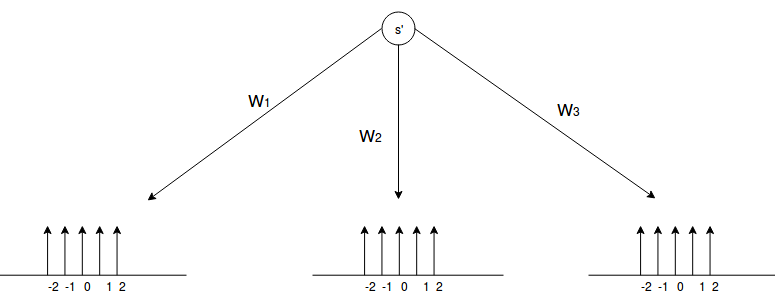
\includegraphics[width=\linewidth]{particles.png}
 \caption{Target Q-distributions of state $s'$.}
 \label{fig:target_distributions}
\end{figure}
Pseudocode of the algorithm is shown in Alg. ~\ref{alg:weighted_updating}. 
\begin{algorithm}[H]
\begin{flushleft}
 \textbf{Input:} A transition $s,a,r,s'$, $\gamma \in [0,1]$, $\alpha \in [0,1]$\\
\end{flushleft}
 \begin{algorithmic}
 
 \For{$j \in 1, \cdots, m$}
 		\State $w_j =\sum_{i=1}^{N} \frac{1}{N} \prod_{a' \neq a} \sum_{x_{a'}^j < x_a^i} \frac{1}{N}$
 \EndFor
 \For{$i \in 1, \cdots, N$}
 		\State $x'^{t}_i(s')= \sum_{j=1}^{m} w_j x'^{t}_i(s',a_j)$ 
 		\State $x^{t+1}_i(s,a) \leftarrow x^{t}_i(s,a) + \alpha (r+\gamma x'^{t}_i(s') - x^{t}_i(s,a))$
 \EndFor
 \end{algorithmic}
 \caption{Weighted Updating}
 \label{alg:weighted_updating}
\end{algorithm}   
\chapter{Experiments}		\label{chap:chapter5}
This chapter is devoted to the evaluation of Particle Q Learning on classic benchmark problems, both in the tabular and in the function approximation cases. In Section ~\ref{sec:tabular_experiments} we show the results of experiments in the tabular case for classic problems found in the literature. Section ~\ref{sec:atari_experiments} describes the experiments performed in the \emph{Arcade Learning Environment} (ALE) ~\cite{Bellemare:2013:ALE:2566972.2566979}, a classic benchmark in the Deep RL literature. 
\section{Tabular Case} \label{sec:tabular_experiments}
This section is devoted to experiments conducted in finite domains where the tabular version of the algorithm can be used. The experiments are done in 6 different domains taken from the literature on efficient and deep exploration. Combining  the two policies (VPI policy and Weighted Policy) with the two update methods (Maximum Mean Updating and Weighted Updating) proposed in the previous chapter we propose four versions of Particle Q-learning. We compare the results produced using these algorithms with the ones produced from different variations of two algorithms from the literature:
\begin{itemize}
\item Q-learning with $\epsilon$-greedy or Boltzmann exploration,
\item Bootstrapped Q-learning with the Bootstrapped policy defined in ~\cite{DBLP:journals/corr/OsbandBPR16} and with the Weighted policy discussed in the previous chapter.
\end{itemize}
For all algorithms we have also considered their ``double'' versions, \ie modifications of the algorithms that use two Q-tables as in ~\cite{Hasselt:2016:DRL:3016100.3016191}. The results of using the ``double'' versions are shown in Appendix~\ref{app:appendixA} 
\subsection{Evaluation Metrics}
In this thesis, we addressed the exploration vs. exploitation dilemma by maintaining Q-distributions and using them to perform more informed decisions. A reinforcement learning agent needs exploration to learn an optimal policy faster in complex domains, but also not to get stuck in sub-optimal policies in domains that except them, and where discovering the optimal policy might be ``trickier''. For this purpose we test our algorithms in 6 domains, some of them designed to be ``tricky'', and some classical navigation problems. We compare algorithms by looking at the learning curve, \ie mean scores collected as a function of the training time. Algorithms that explore better, should not only show faster increasing curves, but also not get stuck in sub-optimal solutions. We show the mean scores over multiple runs, by shadowing around the curves to show also 95\% confidence interval.\par
We will also discuss how the Q-distributions maintained by the agent progress during learning. As we mentioned in the previous Chapter, as learning continues, the distributions should shrink to the true Q-value. We note that if the distributions shrink too quick, the agent might be stuck in a suboptimal policy. For this purpose we will show the following:
\begin{itemize}
\item Particle positions as learning progresses, to see if they do in fact converge,
\item Variance of the Q-distributions, which should converge to 0,
\item Probability of exploration, \ie probability of choosing an action different than the greedy one.
\end{itemize}
The first two of these curves are defined for each $(s,a)$ pair, whereas the last curve is defined for each state.
\subsection{Experimental Setup}
We train each agent for 100 episodes, the length of each episode is domain dependent. During the training periods we collect the rewards and use them to calculate the \emph{online scores}. After each training period, we ``turn off'' exploration and evaluate the policies learned by the agent. The length of the evaluation episodes is the same as the training episodes. We use the rewards collected during evaluation to calculate the \emph{offline scores}. We perform this process in each domain, for each algorithm considered and show the mean scores of 10 runs. We calculate the undiscounted scores, even though we use a discount factor in each domain during learning.\par
For our particle algorithms, we initialize the particles equally spaced in an interval $[q_{min}, q_{max}]$, for each state action-pair. The range of this interval is problem dependent and we see these hyper parameters as a way to incorporate prior knowledge about the domain. We consider Bootstrapped Q-learning with two policy models, the Bootstrapped policy defined in \cite{DBLP:journals/corr/OsbandBPR16} and the weighted policy. We initialize the Q-tables with values drawn from a Gaussian distribution with parameters $\mu=\frac{q_{min}+q_{max}}{2},\sigma=q_{max}-q_{min}$. Furthermore, we consider Q-learning algorithm with $\epsilon$-greedy and Boltzmann exploration. In both Q-learning versions, the Q-table is initialized to 0.\par
For all algorithms we use a \emph{exponentially decaying} learning rate given by:
\begin{equation}
\label{eq:exponential_decay}
\alpha(s,a) = \frac{b}{t(s,a)^a},
\end{equation}
where $t(s,a)$ is the visit count for state-action pair $(s,a)$, $b$ is the initial value which we set to 1 and $a$ is the \emph{decay exponent}. For all our experiments we used $a=0.2$, as it gave us better results.\par
For the Q-learning algorithms we had to chose also the schedules for $\epsilon$ and $\beta$, for $\epsilon$-greedy and Boltzmann exploration respectively. For $\epsilon$ we used an exponetially decaying schedule as in (\ref{eq:exponential_decay}) with $b=1$ and $a=0.5$ whereas for the Boltzmann policy we used an exponentially decaying $\beta$ with initial value, $b=1.5q_{max}$ and decay exponent, $a=0.5$. 
\subsection{Chain Domain}
The first domain we describe, taken from~\cite{Dearden98bayesianq-learning}, is shown in Figure~\ref{fig:chain_domain}. The domain is composed of 5 states, labeled from 1 to 5. The agent can choose between two actions in each domain, labeled as $a$, $b$ (represented in the figure as the edges). The labels in the edges represent the action executed and the reward collected from the transition. With probability $p=0.2$ each action ``fails'' and the opposite action is executed instead, \ie we observe reward $r$ and next-state $s'$ of the opposite action. The domain is designed to test exploration approaches. Assuming a discount factor $\gamma=0.99$, the optimal policy is to always execute action $a$ to receive the high reward at the last state. If the agent does not explore enough it could be stuck in the suboptimal policy of executing always $b$ and collecting the smaller reward of 2.
\begin{figure}
 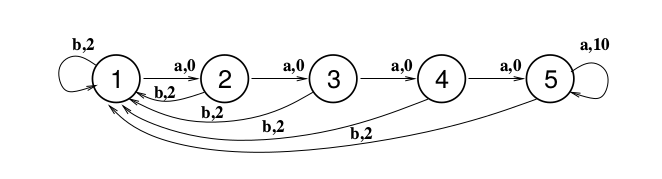
\includegraphics[width=\linewidth]{chain_domain.png}
 \caption{Chain domain taken from ~\cite{Dearden98bayesianq-learning}.}
 \label{fig:chain_domain}
\end{figure}
\begin{figure}
 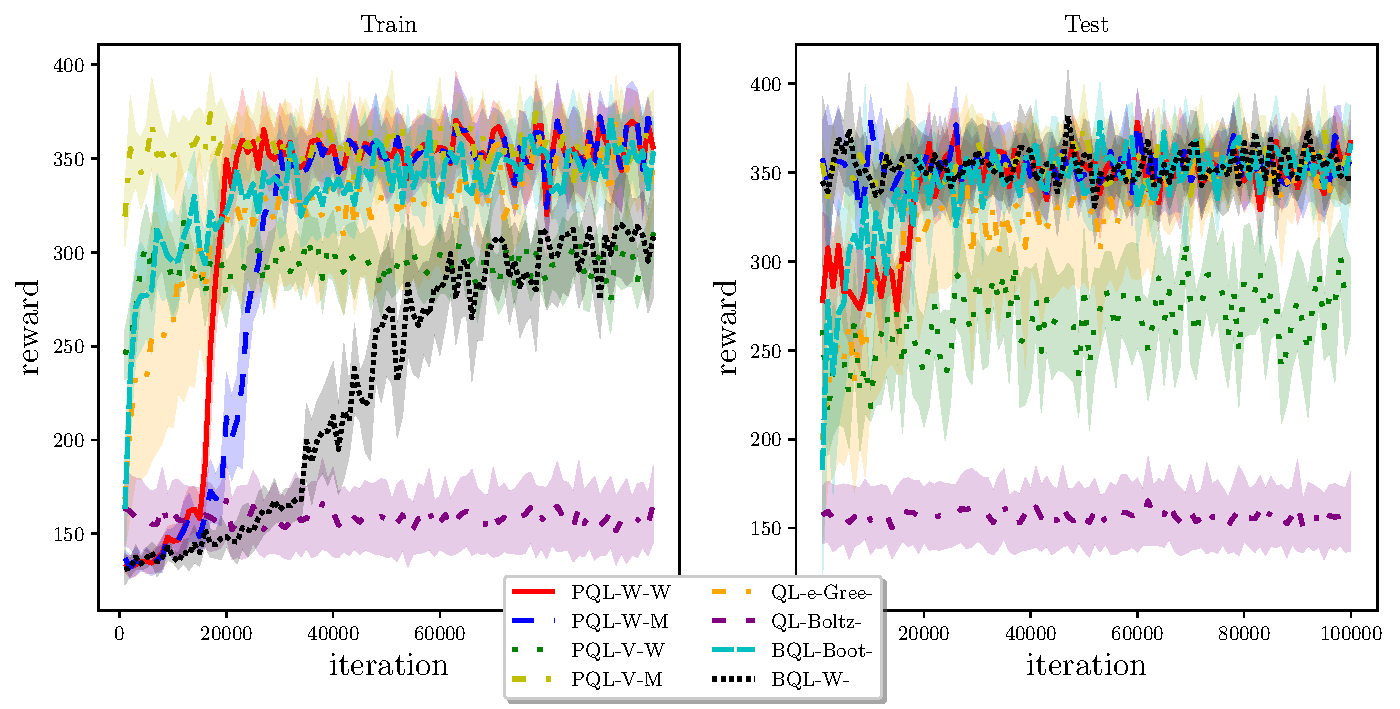
\includegraphics[width=\linewidth]{Chain/learning_curve.pdf}
 \caption{Online (left) and offline (right) scores in the Chain domain.}
 \label{fig:chain_learning_curve}
\end{figure}
Figure~\ref{fig:chain_learning_curve} shows the results of our tests in the Chain domain. We trained each agent for 100 episodes of 1000 timesteps, for a total of 100000 timesteps. The scores collected during training are shown in the left plots. After each training periods, we evaluated the agents for another 1000 steps. During evaluation agents stopped exploring and followed the greedy policies instead. This was done to evaluate the policies derived if training finished at that moment. The plots show the mean score of 10 independent runs and the shaded regions around the line, represent the 95\% confidence interval of the mean.\par
\begin{figure}
\centering
\begin{subfigure}{\linewidth}
  \centering
  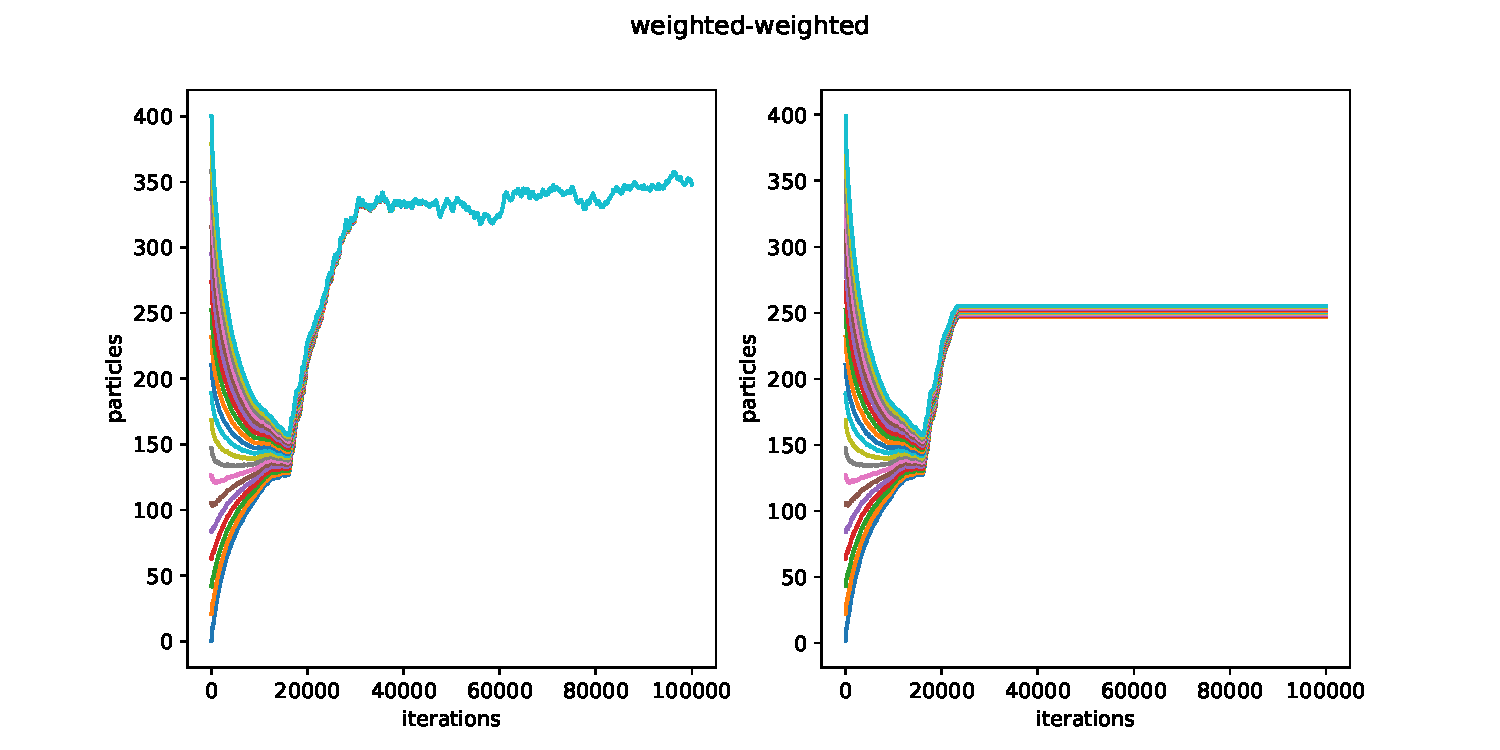
\includegraphics[width=\linewidth]{Chain/particles_weighted-weighted.pdf}
  \caption{}
  \label{fig:chain_particles_weighted_weighted}
\end{subfigure}%

\bigskip
\centering
\begin{subfigure}{\linewidth}
  \centering
  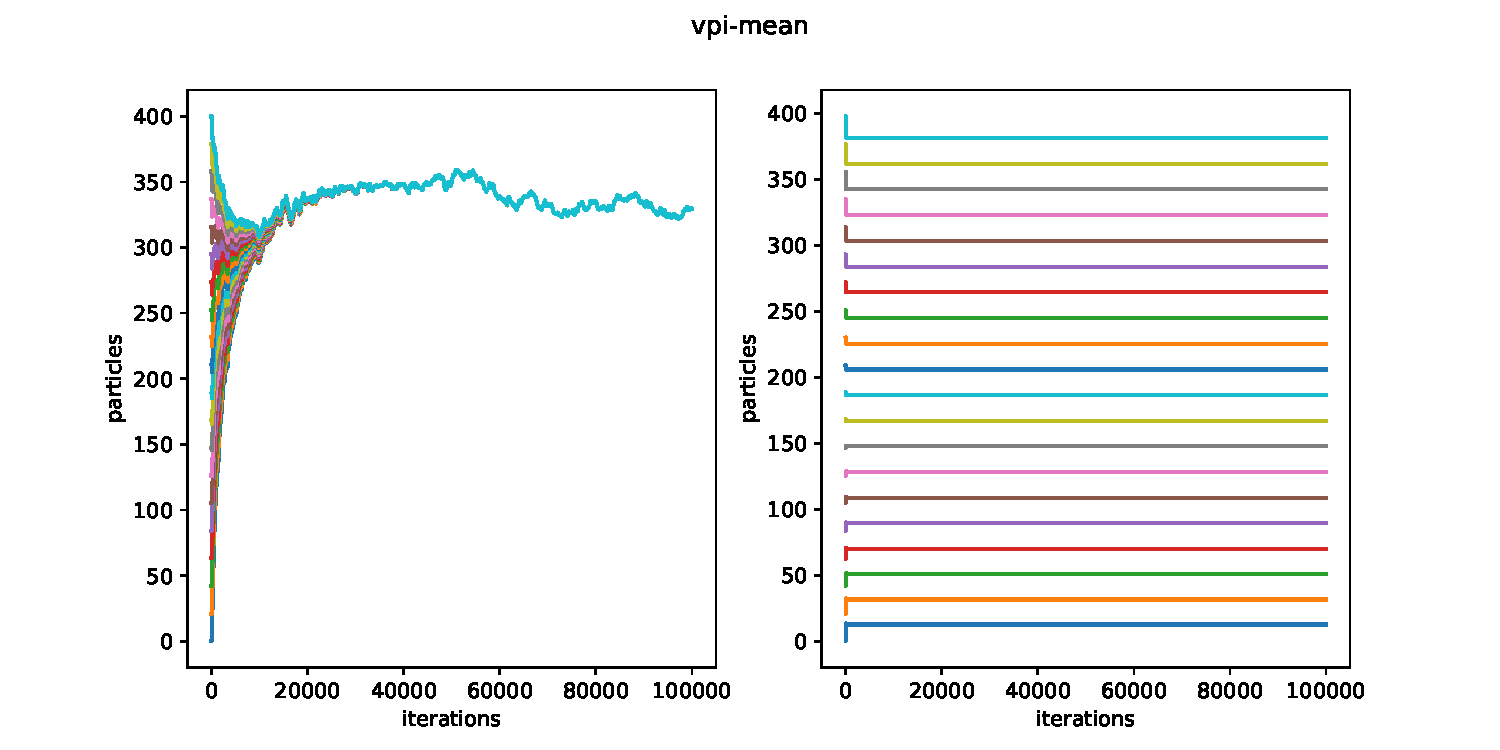
\includegraphics[width=\linewidth]{Chain/particles_vpi-mean.pdf}
   \caption{}
   \label{fig:chain_particles_vpi_mean}
\end{subfigure}
\caption{Evolution of the particles in the first state of the Chain domain during the learning process for the Particle Q-learning algorithm with weighted policy and weighted update (a), and VPI policy and maximum mean update (b). The optimal action \emph{a} is shown on the left, while the suboptimal action \emph{b} is shown on the right on both (a) and (b).}
\label{fig:chain_particle_evolution}
\end{figure}
We can understand immediately from the picture that simple exploration strategies, like Boltzmann, fail to solve this simple domain. If we consider the online case, \ie how the agent behaves during training, our algorithm, Particle Q-learning, used with VPI policy and maximum mean update, has the best performance, scoring the maximum possible since the beginning of learning. We can note that bootstrapped Q-learning (BQL) starts good at the beginning and then its performance is surpassed by the performance of our algorithms using the weighted policy, with both update methods (weighted and maximum mean). We evaluated also another version of BQL, which used the weighted policy. We can see that in the online case, this algorithm did not perform well. It is interesting that, in the offline evaluation, BQL performed really well since the beginning. This means that while it learned the optimal policy quickly, it failed to send exploration to zero fast enough. This is something we will see also in the next experiments.\par
We will now discuss how the particles evolve during time. As mentioned before the desired behaviour is that the particles converge to the real Q-value. Obviously, at this point, the algorithm will stop exploring. Figure~\ref{fig:chain_particle_evolution} shows the evolution of the particles in the first state during learning for two versions of our algorithm. We could show these plots for all state-action pairs but for space considerations we are only showing the particles in the first state for both actions. We made this choice because the first state is the most difficult state to learn because it is the closest to the small reward and the furthest from the high reward. \par
\begin{figure}
\centering
\begin{subfigure}{\linewidth}
  \centering
  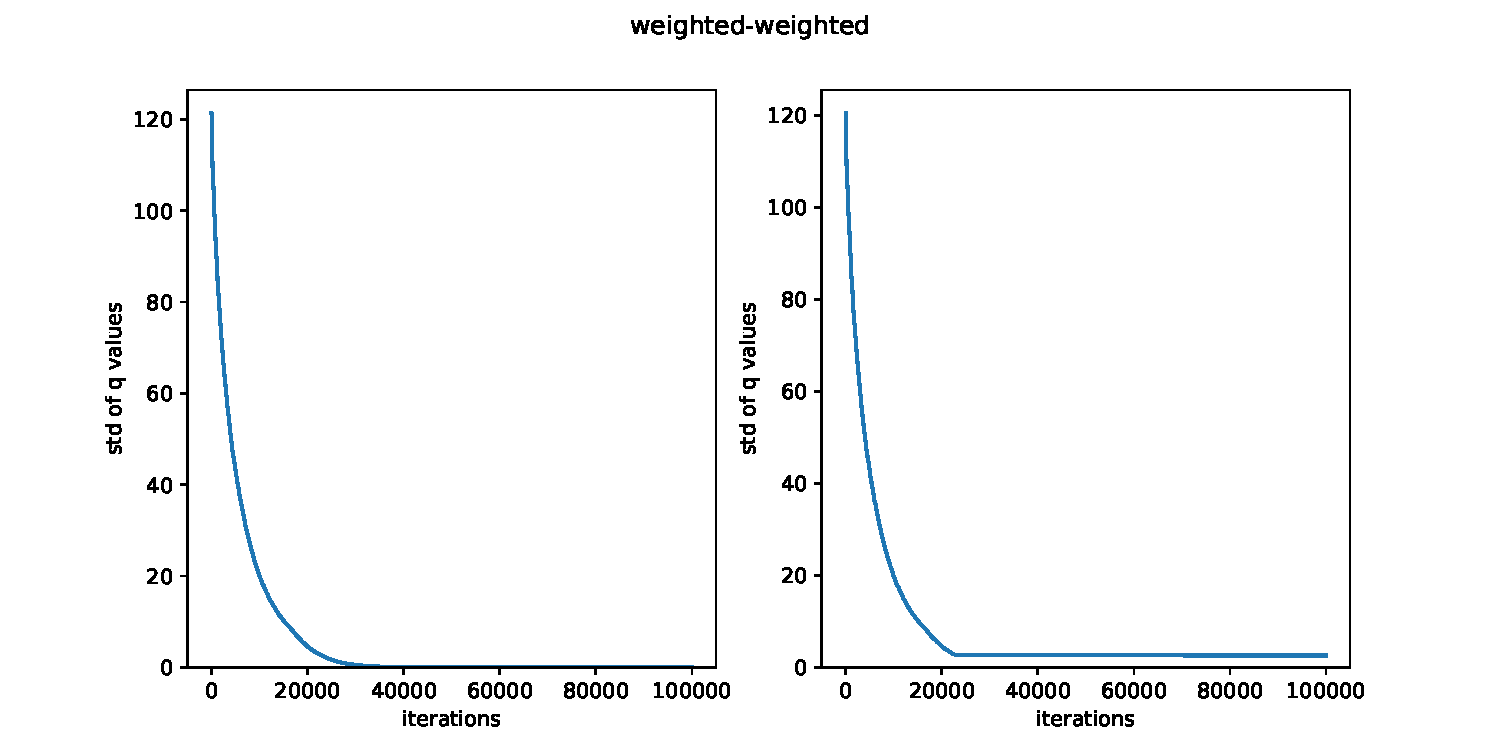
\includegraphics[width=\linewidth]{Chain/std_weighted-weighted.pdf}
  \label{fig:chain_std_weighted_weighted}
  \caption{}
\end{subfigure}

\bigskip
\centering
\begin{subfigure}{\linewidth}
  \centering
  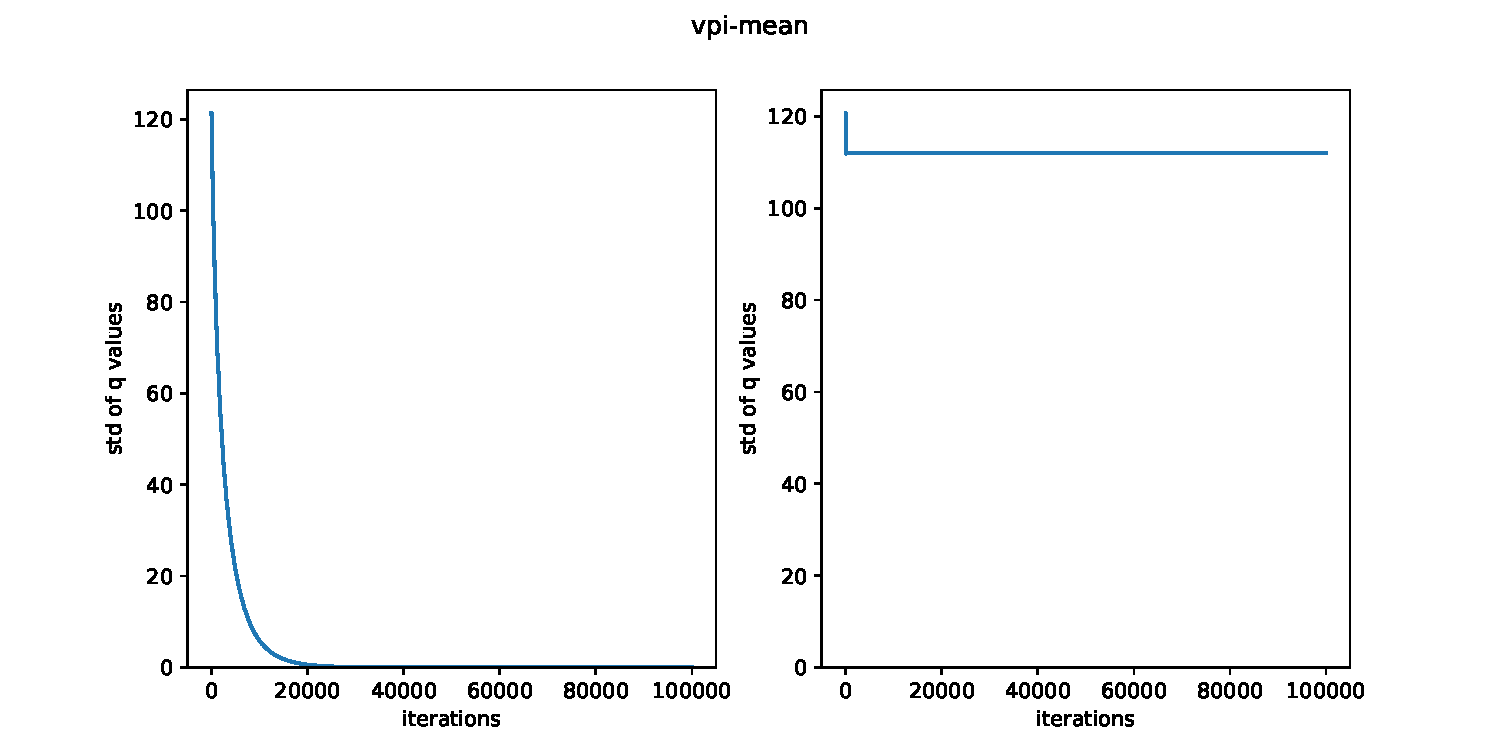
\includegraphics[width=\linewidth]{Chain/std_vpi-mean.pdf}
  \label{fig:chain_std_vpi_mean}
  \caption{}
\end{subfigure}
\caption{Standard deviation of the particles as a function of the learning timestep for the Particle Q-learning algorithm with weighted policy and weighted update (a), and VPI policy and maximum mean update (b). Once again, the optimal action \emph{a} is shown on the left, while the suboptimal action \emph{b} is shown on the right on both (a) and (b).}
\label{fig:chain_std_evolution}
\end{figure}
In Figure~\ref{fig:chain_particles_weighted_weighted}, we can see that for Particle Q-learning with weighted policy and weighted update (PQL\_W\_W), the particles shrink during learning, and after the step 20000, action $b$ is not explored anymore and its particles remain constant. Particle Q-learning with VPI policy and maximum mean update (PQL\_V\_M), shown in Figure~\ref{fig:chain_particles_vpi_mean}, shrinks the particles much faster in the optimal action (left subplot) whereas never shrinks the ones of the suboptimal action. This means that VPI policy stops exploring actions before the uncertainty of their Q-value goes to zero. In this simple domain this gave higher results faster, but in more complicated domains this might lead to premature convergence of the algorithm. This can be seen also in Figure~\ref{fig:chain_std_evolution} where the standard deviation of the particles in the same state is shown for both algorithms. While in the PQL\_W\_W case the standard deviation goes to zero for both actions, in the PQL\_V\_M case only the first action goes to 0. The particles of action $b$ remain spread and the standard deviation remains constant. This is explained by the fact that VPI policy does not consider this action worth exploring even though it is not completely sure about its value, as explained in the previous chapter. we note that while PQL\_V\_M brought good results in this domain, the fact that the actions are not fully explored, and as a result the particles do not shrink, might bring premature convergence in more complex domains.\par
\begin{figure}
  \centering 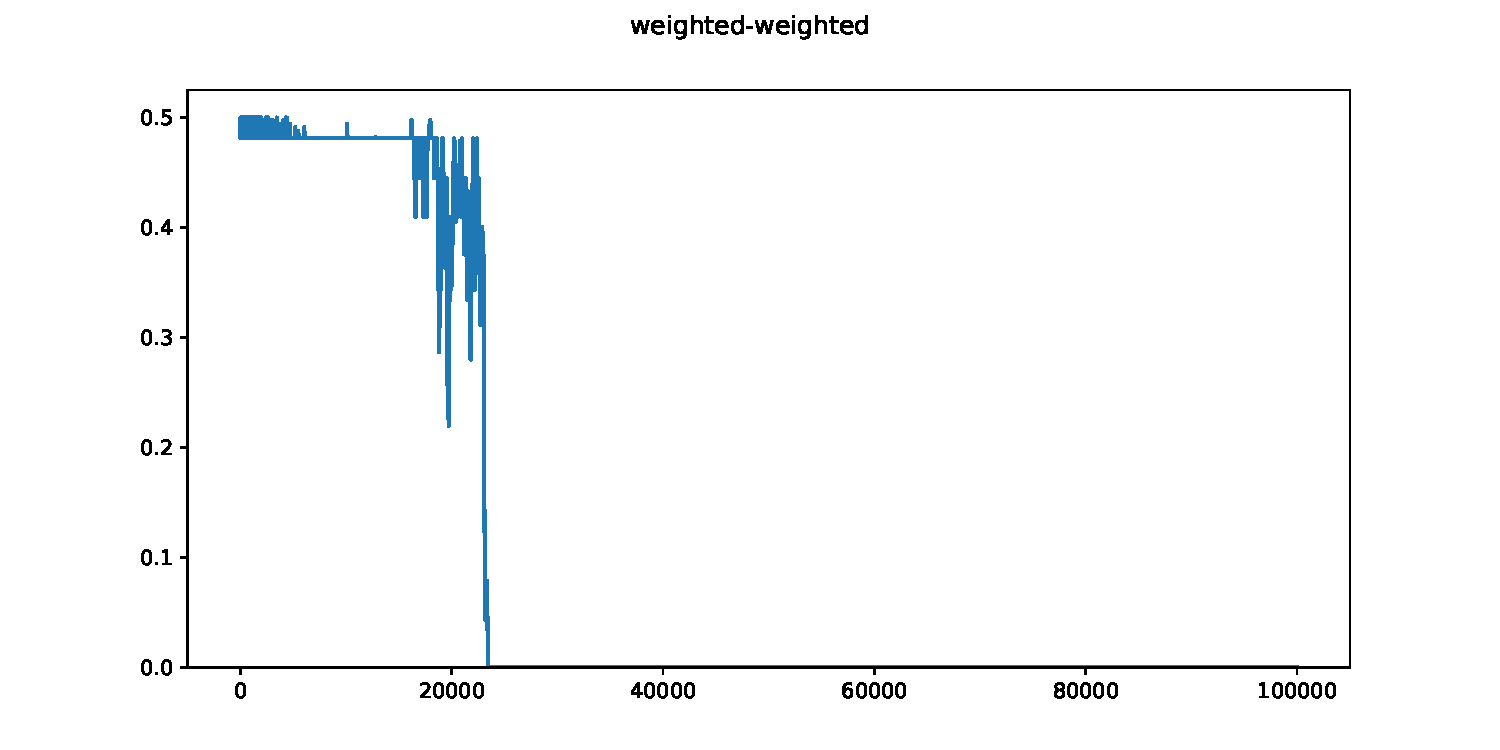
\includegraphics[width=\linewidth]{Chain/prob_weighted-weighted.pdf}
\caption{Probability of exploration as a function of the learning timestep for the Particle Q-learning algorithm with weighted policy and weighted update in the Chain domain.}
\label{fig:chain_prob_evolution}
\end{figure}
Finally we show how the probability of exploration evolves as learning continues. Again we recall that the probability should go to 0, as we go closer the true Q-value. Figure~\ref{fig:chain_prob_evolution} displays our results for PQL\_W\_W. Again we consider just the first state. Same plots could be shown for all states of the domain. We can see that  the probability of exploration goes to 0.

\subsection{Loop Domain}
The second domain we consider, shown in Figure ~\ref{fig:loop_domain}, is also taken from~\cite{Dearden98bayesianq-learning}. Similar to the first domain, the agent has 2 available actions in each of the 9 states. The name comes from the fact that, starting from the initial state 0, the agent has to choose between the two loops available. All rewards are 0, except the last transitions of the loops. The agent has to learn to perform the left loop, which gives the highest reward, but the right loop, although suboptimal, is easier to reach. An agent that does not explore enough might be stuck in the suboptimal loop.\par
\begin{figure}
 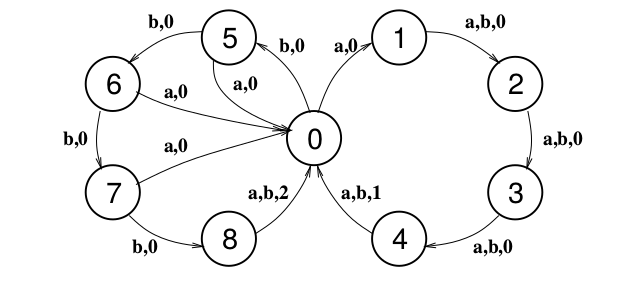
\includegraphics[width=\linewidth]{loop_domain.png}
 \caption{Loop domain taken from ~\cite{Dearden98bayesianq-learning}.} 
 \label{fig:loop_domain}
\end{figure}
\begin{figure}
 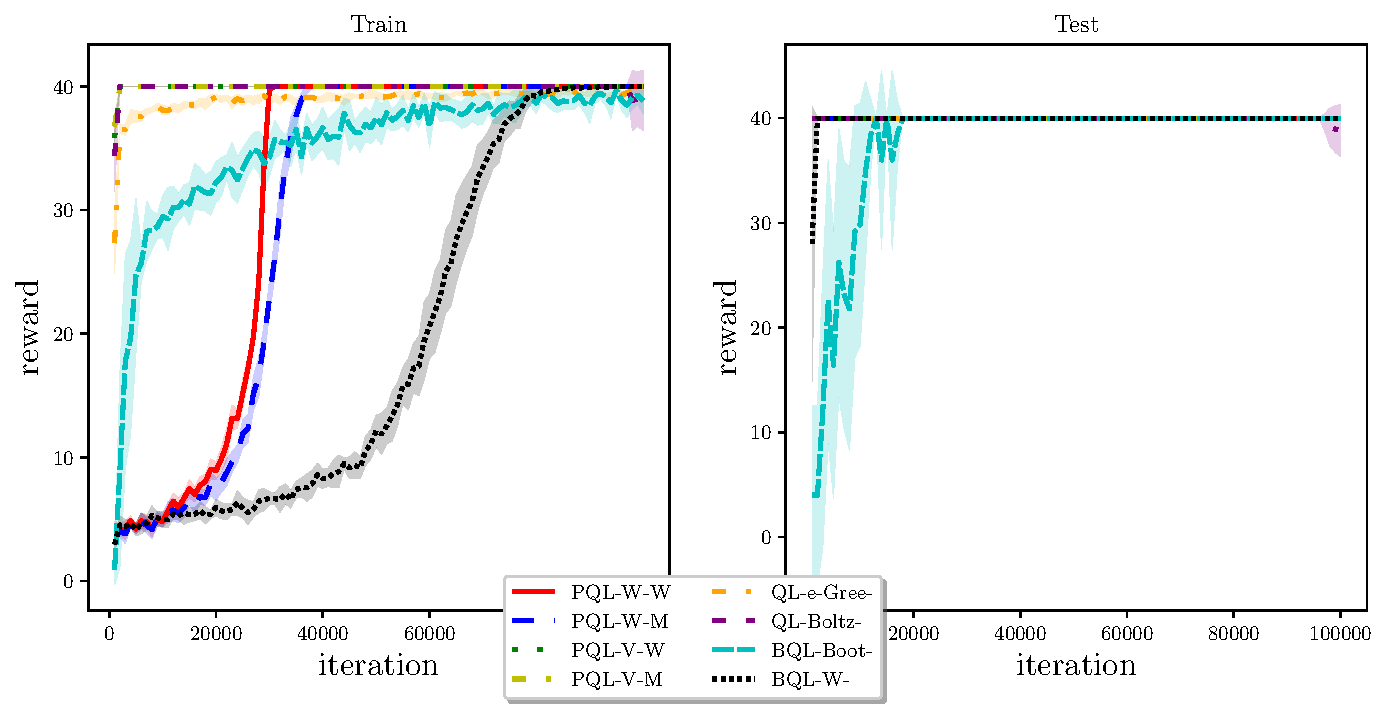
\includegraphics[width=\linewidth]{Loop/learning_curve.pdf}
 \caption{Online and offline scores in the Loop domain.}
 \label{fig:loop_learning_curve}
\end{figure}
Figure~\ref{fig:loop_learning_curve} shows the results of our tests in the Loop domain. Again we trained each agent for 100 episodes of 1000 timesteps, for a total of 100000 timesteps and display the online and offline undiscounted scores. This domain is slightly more simple than Chain. Indeed simple exploration approaches like Boltzmann or $\epsilon$-greedy perform well in this domain. Nonetheless, PQL with VPI policy performs best in both offline and online cases, while the versions using weighted policy learn slower due to the fact that they explore actions until they are sure about their value. We can see that boostrapped Q-learning starts better than these algorithms, but its performance is surpassed later. We will also discuss the behaviour of the particles as before. \par
\begin{figure}
\centering
\begin{subfigure}{\linewidth}
  \centering
  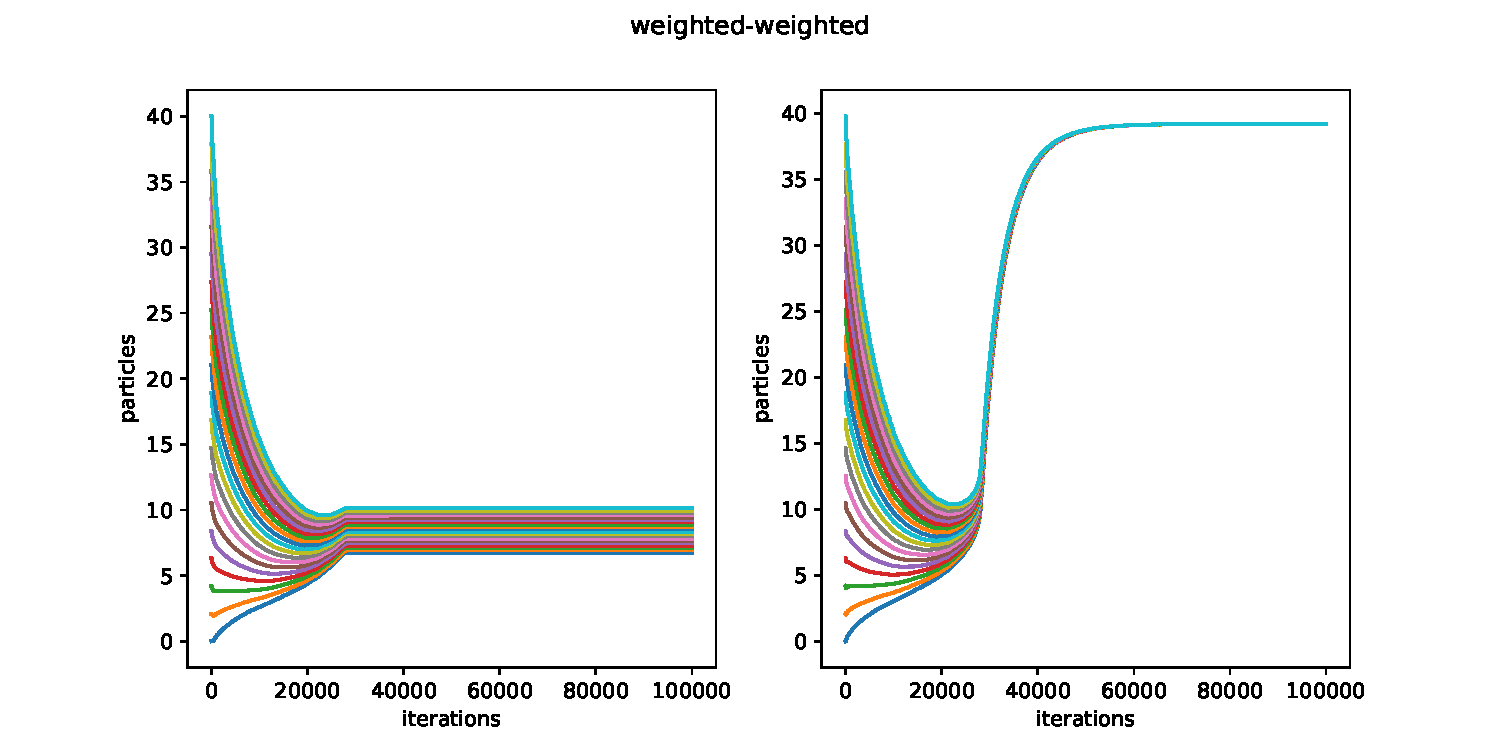
\includegraphics[width=\linewidth]{Loop/particles_weighted-weighted.pdf}
  \label{fig:loop_particles_weighted_weighted}
  \caption{}
\end{subfigure}%

\bigskip
\centering
\begin{subfigure}{\linewidth}
  \centering
  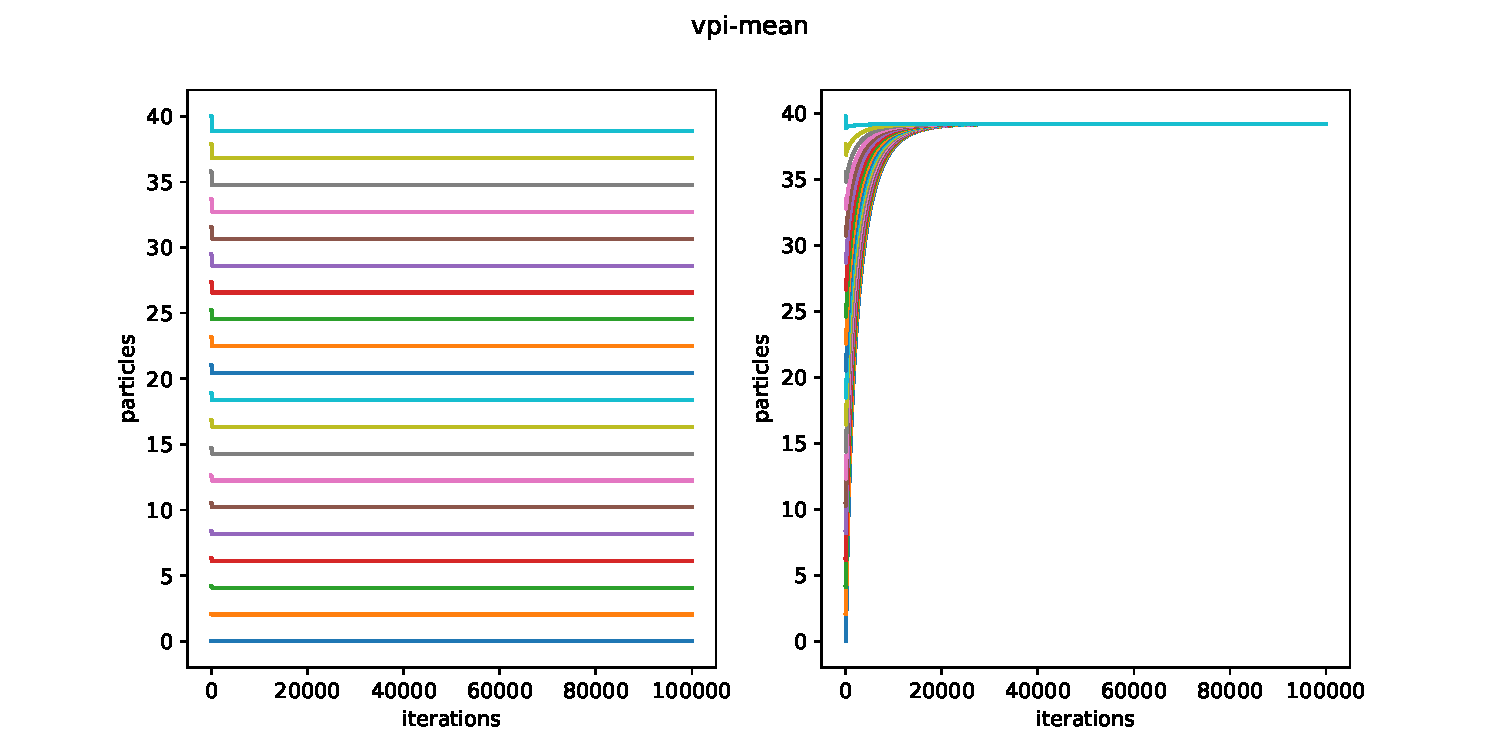
\includegraphics[width=\linewidth]{Loop/particles_vpi-mean.pdf}
  \caption{}
  \label{fig:loop_particles_vpi_mean}
\end{subfigure}
\caption{Evolution of the particles in the first state of the Loop domain during the learning process for the Particle Q-learning algorithm with weighted policy and weighted update (a), and VPI policy and maximum mean update (b). The optimal action \emph{b} is shown on the right, while the suboptimal action is shown on the left on both (a) and (b).}
\label{fig:loop_particle_evolution}
\end{figure}
Again we will consider just the first state as it is the state where we have to choose which loop to execute. Figure~\ref{fig:loop_particle_evolution} shows a situation similar to the Chain domain. While PQL\_W\_W explores actions until the uncertainty of the Q-values shrinks, PQL\_V\_M stops exploring when it estimates that there is no added value in executing actions. We can see this in Figure~\ref{fig:loop_particles_vpi_mean} where the particles of the suboptimal action remain spread, so the action is not explored further. Figure~\ref{fig:loop_std_evolution} shows the standard deviation of the particles. Again this converges in both action in the PQL\_W\_W case but in PQL\_V\_M, the standard deviation of the particles of the suboptimal action remains large.\par
\begin{figure}
\centering
\begin{subfigure}{\linewidth}
  \centering
  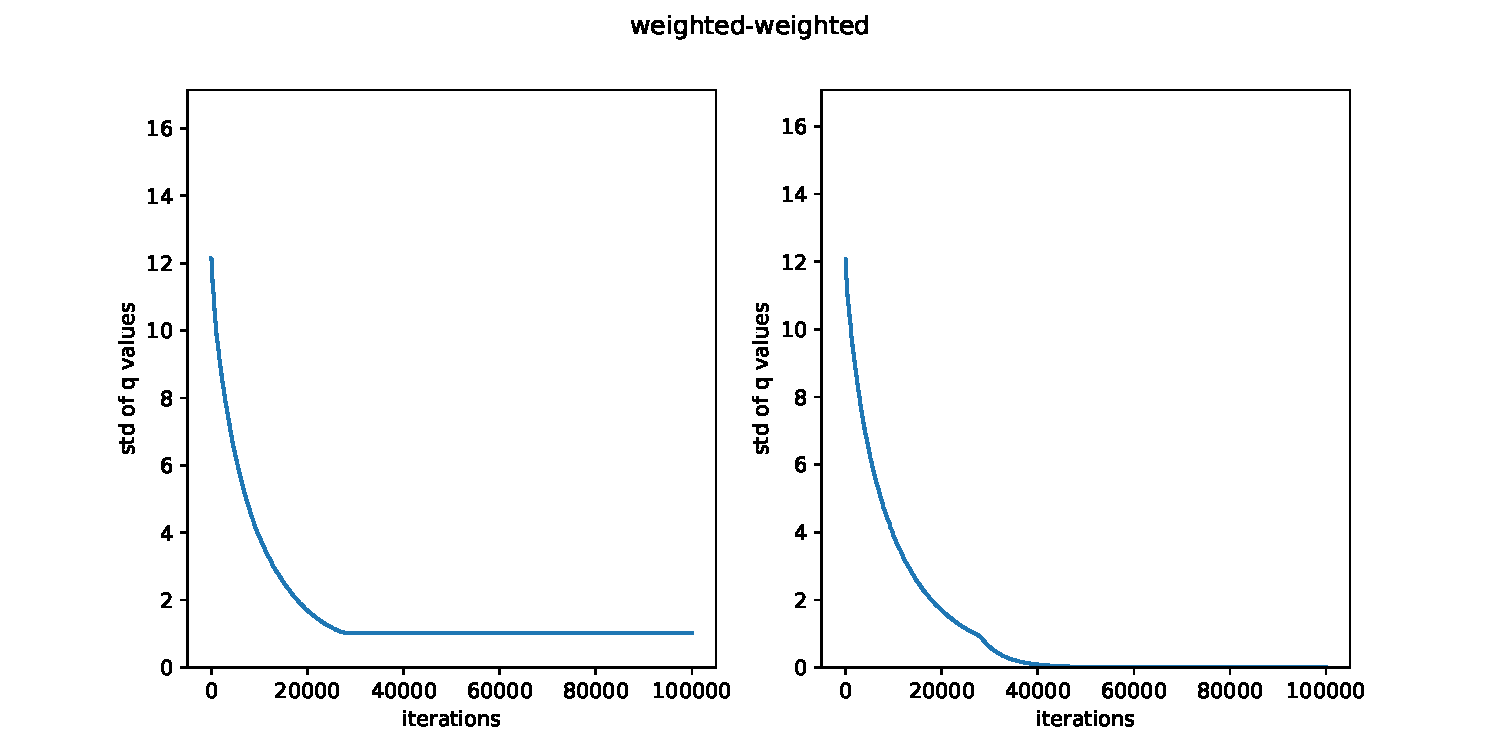
\includegraphics[width=\linewidth]{Loop/std_weighted-weighted.pdf}
  \label{fig:loop_std_weighted_weighted}
  \caption{}
\end{subfigure}

\bigskip
\centering
\begin{subfigure}{\linewidth}
  \centering
  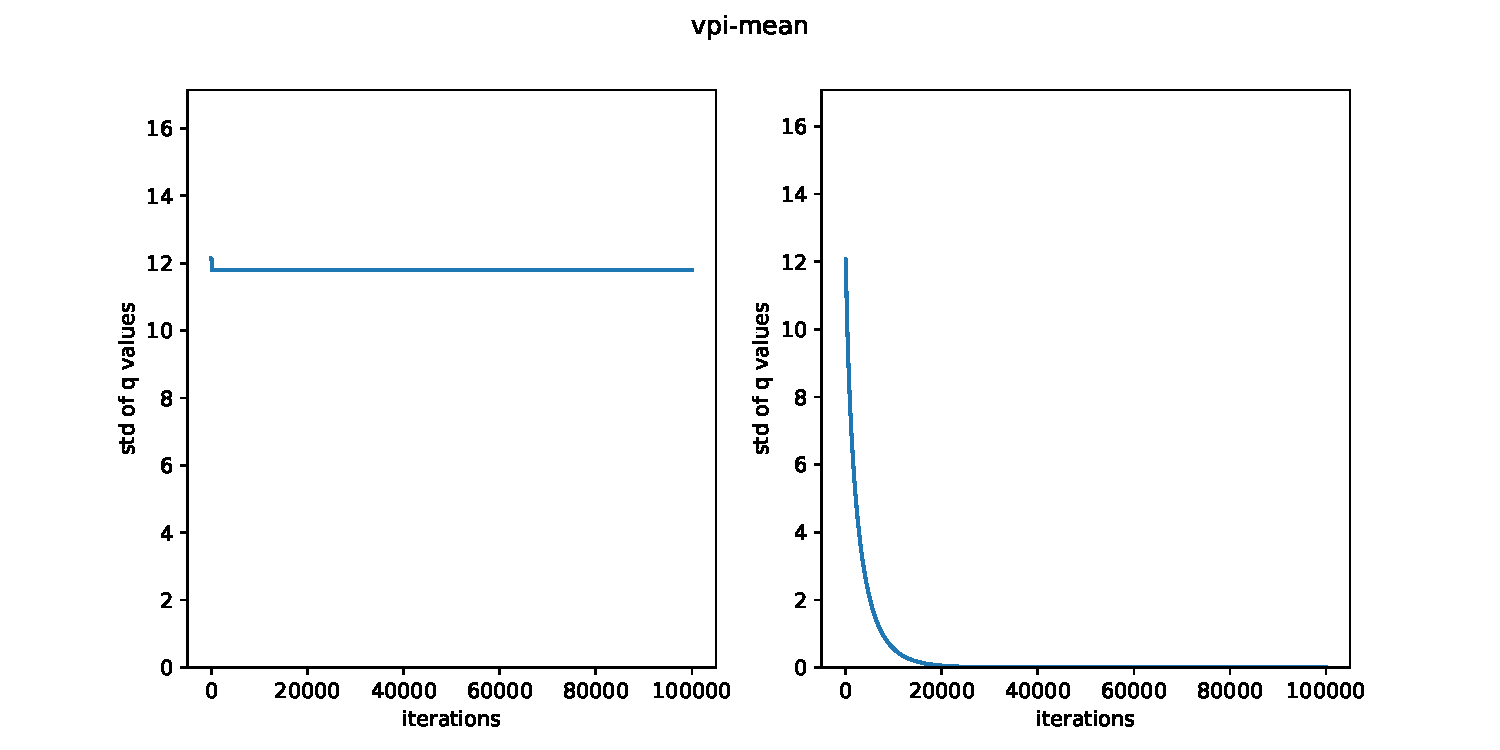
\includegraphics[width=\linewidth]{Loop/std_vpi-mean.pdf}
  \label{fig:loop_std_vpi_mean}
  \caption{}
\end{subfigure}
\caption{Standard deviation of the particles as a function of the learning timestep for the Particle Q-learning algorithm with weighted policy and weighted update (a), and VPI policy and maximum mean update (b) in the Loop domain. The optimal action  is shown on the right, while the suboptimal action is shown on the left on both (a) and (b).}
\label{fig:loop_std_evolution}
\end{figure}
Finally, Figure~\ref{fig:loop_prob_evolution} shows the probability of exploring as a function of the timesteps. As before, in the PQL\_W\_W the probability of exploration goes to 0.
\begin{figure}
  \centering
  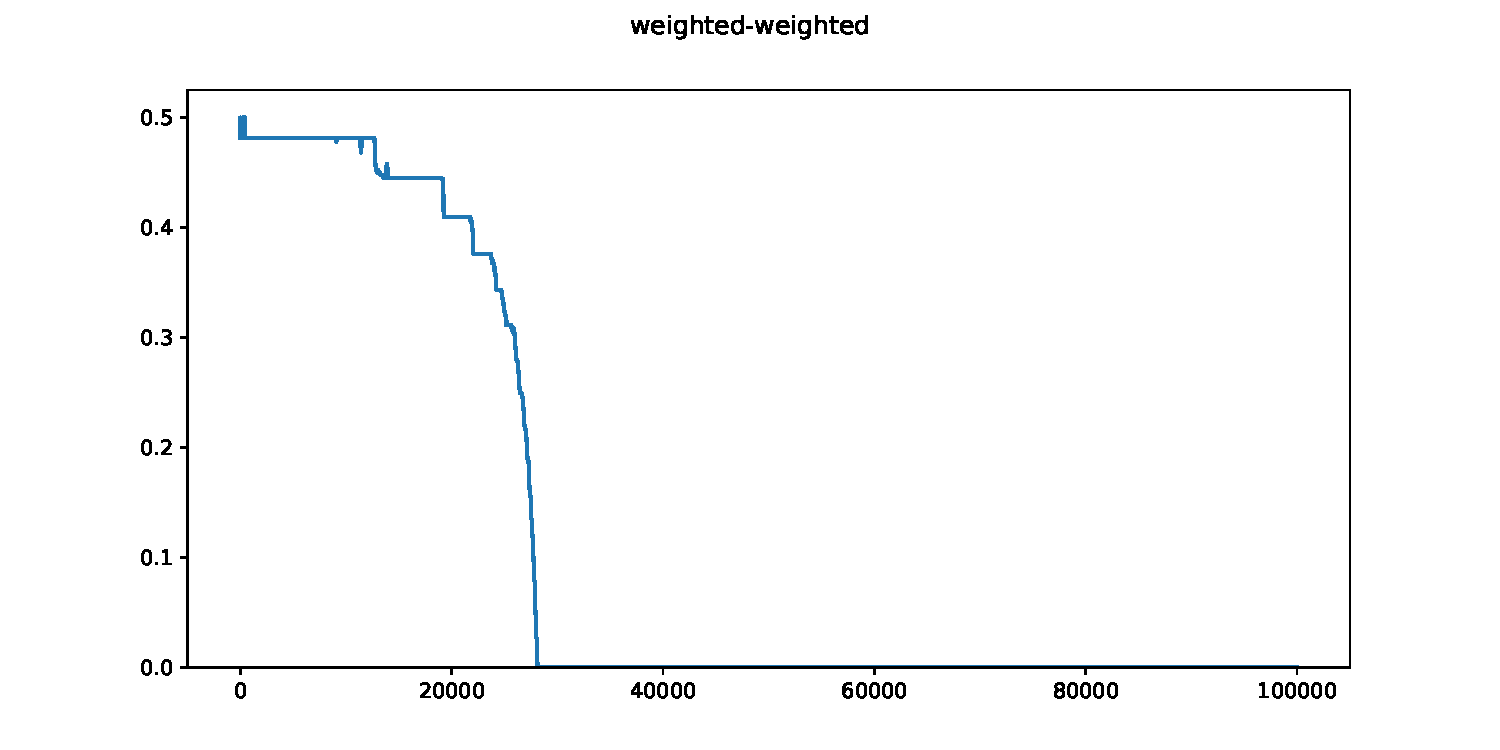
\includegraphics[width=\linewidth]{Loop/prob_weighted-weighted.pdf}
\caption{Probability of exploration as a function of the learning timestep for the Particle Q-learning algorithm with weighted policy and weighted update in the Loop domain.}
\label{fig:loop_prob_evolution}
\end{figure}
\subsection{Taxi Domain}
We will now review our results in the Taxi domain. This domain is a classical benchmark for exploration in literature and has different versions. We will consider the version taken from \cite{Dearden98bayesianq-learning} where it appears as the Maze domain. The domain is shown in Figure ~\ref{fig:taxi_domain}.\par 
Taxi is a navigation problem. The environment is a $5\times5$ grid with 5 special locations labeled by different letters (S,F,F,F,G). The agent starts from cell $S$ (start). The objective of the agent is to pick up passengers, situated at the F (flag) locations and drop them off at the goal location (G). The reward is zero for every transition except when the goal is reached, where the reward collected depends on the number of passengers the agent has picked up. When the agent reaches the goal, the reward is 0, 1, 3, 15 for 0, 1, 2 and 3 passengers collected respectively.\par 
The agent has 4 possible actions, up, down, left and right. The agent picks up passengers by going in their location, but does not observe the reward until it reaches the goal state. The environment also has walls in some locations. When an agent performs an action that would transition into a location occupied from a wall, the agent does not change its location. Finally, each action has a 0.1 probability of ``failing''. When an action fails, the agent goes in a perpendicular direction instead. The challenge of the domain is to do sufficient exploration and collect all passengers before going to the goal.\par
\begin{figure}
 \centering 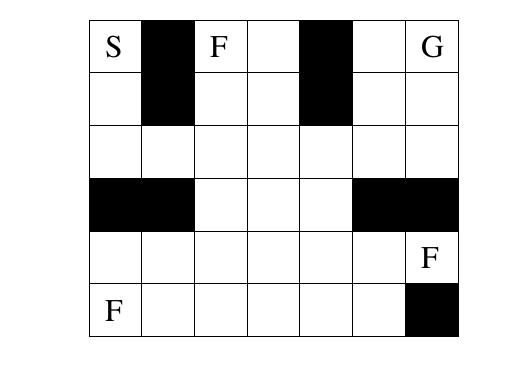
\includegraphics[width=.7\linewidth]{taxi_domain.png}
 \caption{Taxi domain taken from ~\cite{Dearden98bayesianq-learning}, where it appears as the Maze domain.} ~
 \label{fig:taxi_domain}
\end{figure}
\begin{figure}
 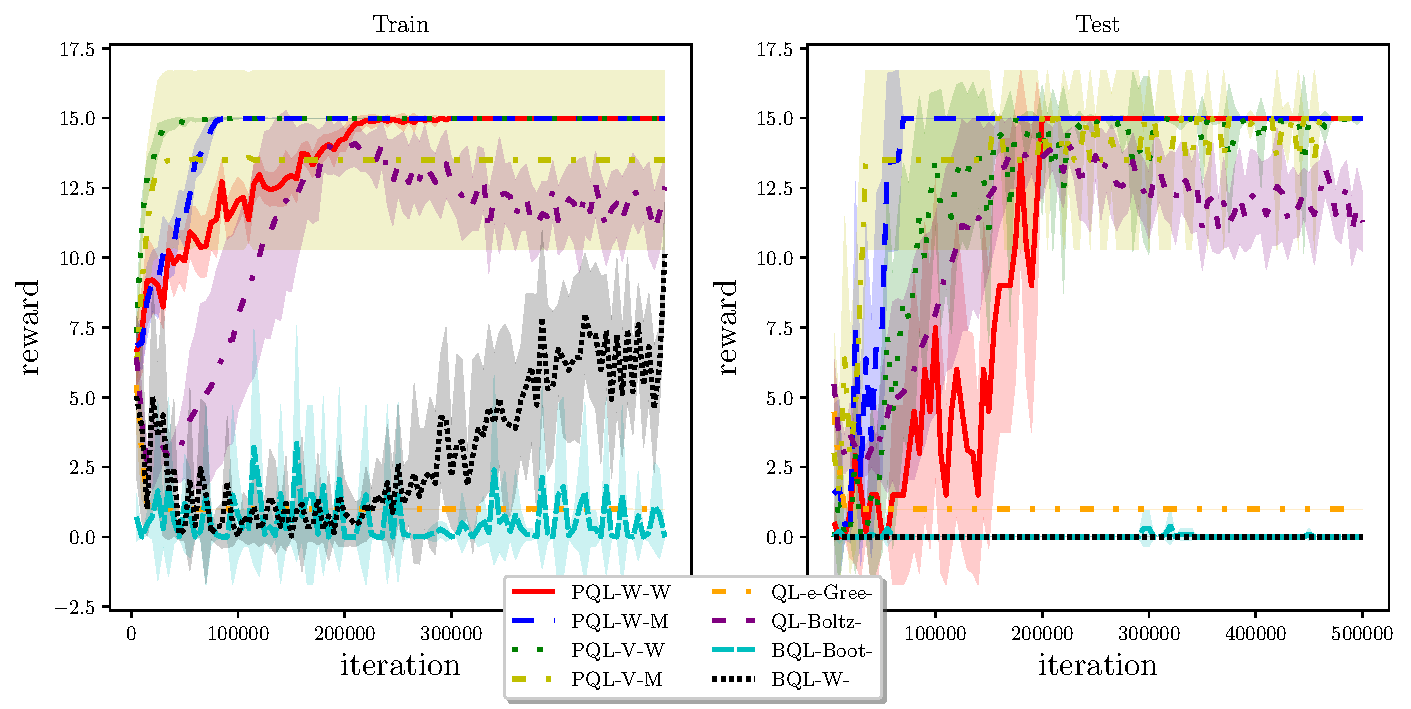
\includegraphics[width=\linewidth]{Taxi/learning_curve.pdf}
 \caption{Online and offline scores in the Taxi domain.}
 \label{fig:taxi_learning_curve}
\end{figure}
Figure~\ref{fig:taxi_learning_curve} shows the results of our tests in the Taxi domain. We considered again 100 training episodes, but with 5000 training steps each. We increased the size of the training periods to allow the agent to reach the goal multiple times in the first steps. We found that smaller training episodes might prevent the agent from learning, since it will not reach the goal before the end of the episode.\par
We can see immediately that BQL performs extremely badly in this domain. The agent scores zero because it does not learn to reach the goal. Instead it moves around the grid during the whole duration of the experiments. Q-learning with $\epsilon$-greedy also performs poorly as it learns to pick-up only a single passenger. Surprisingly enough, Q-learning with Boltzmann exploration performs better. The best performance is shown by all 4 versions of PQL, which quickly learn to pick-up all the passengers, even if with different learning speeds. Again, the versions using weighted policy are fairly slower than the rest of the algorithms due to the fact that they explore the actions until the uncertainty about their Q-values is low enough. This might lead to unnecessary exploration as in the first two domains.
\subsection{River Swim Domain }
The next domain we consider is the River Swim domain, taken from ~\cite{Strehl2008AnAO}. The environment is shown in Figure ~\ref{fig:riverswim_domain}. The MDP consists of six states numbered 1 to 6. The two actions available to the agent are to swim left or right represented by the edges in the figure. The agent starts in one of the states near the beginning of the row. Swimming to the right (against the current of the river) will more often than not leave the agent in the same state, but will sometimes transition the agent to the right (and with a much smaller probability to the left). Swimming to the left (with the current) always succeeds in moving the agent to the left, until the leftmost state is reached at which point swimming to the left yields a small reward of five units. The agent receives a much larger reward, of ten thousand units, for swimming upstream and reaching the rightmost state. The $(a,p,r)$ labels next to the edges in Figure~\ref{fig:riverswim_domain} represent the action, probability of success and reward tuple. For example, the label (1,0.7,0) next to the edge from node 0 to node 0 means that when executing action 1 from state 0 there is a 0.7 probability of staying in node 0 and receiving reward 0 and a 0.3 probability of transitioning to state 1 and receiving again reward 0.\par
\begin{figure}
 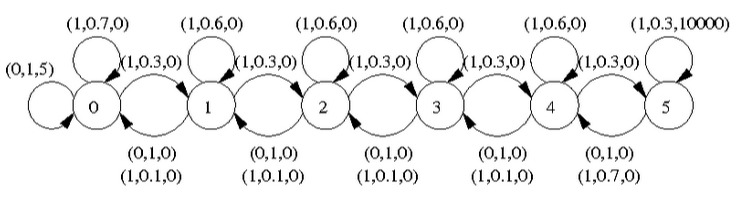
\includegraphics[width=\linewidth]{riverswim_domain.jpeg}
 \caption{River Swim domain taken from ~\cite{Strehl2008AnAO}.} ~
 \label{fig:riverswim_domain}
\end{figure}
\begin{figure}
 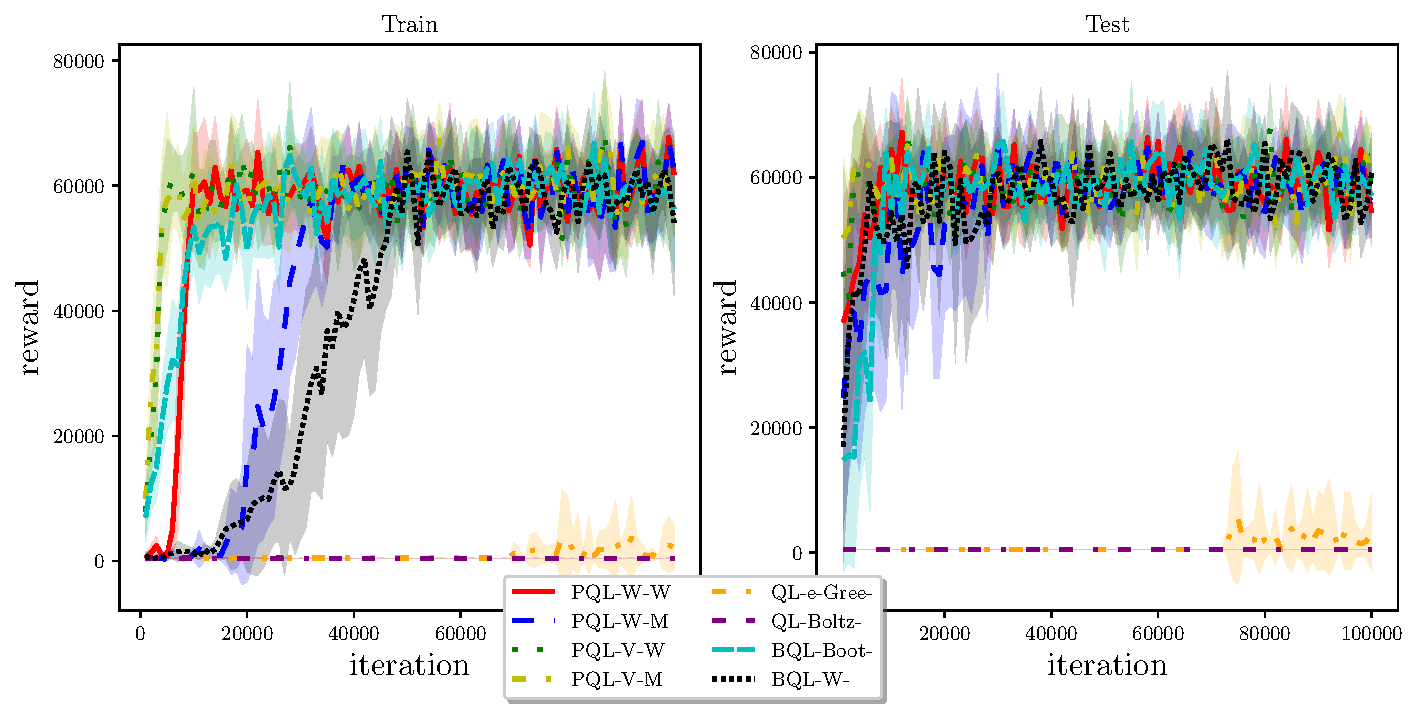
\includegraphics[width=\linewidth]{RiverSwim/learning_curve.pdf}
 \caption{Online and offline scores in the River Swim domain.}
 \label{fig:riverswim_learning_curve}
\end{figure}
Figure~\ref{fig:riverswim_learning_curve} shows the results of our tests in the River Swim domain. The length of the training episodes is 1000 timesteps. We train each agent for 100 episodes and show the undiscounted online and offline scores. This domain is the first of our tests where the simple exploration methods completely fail. \par
\begin{figure}
\centering
\begin{subfigure}{\linewidth}
  \centering
  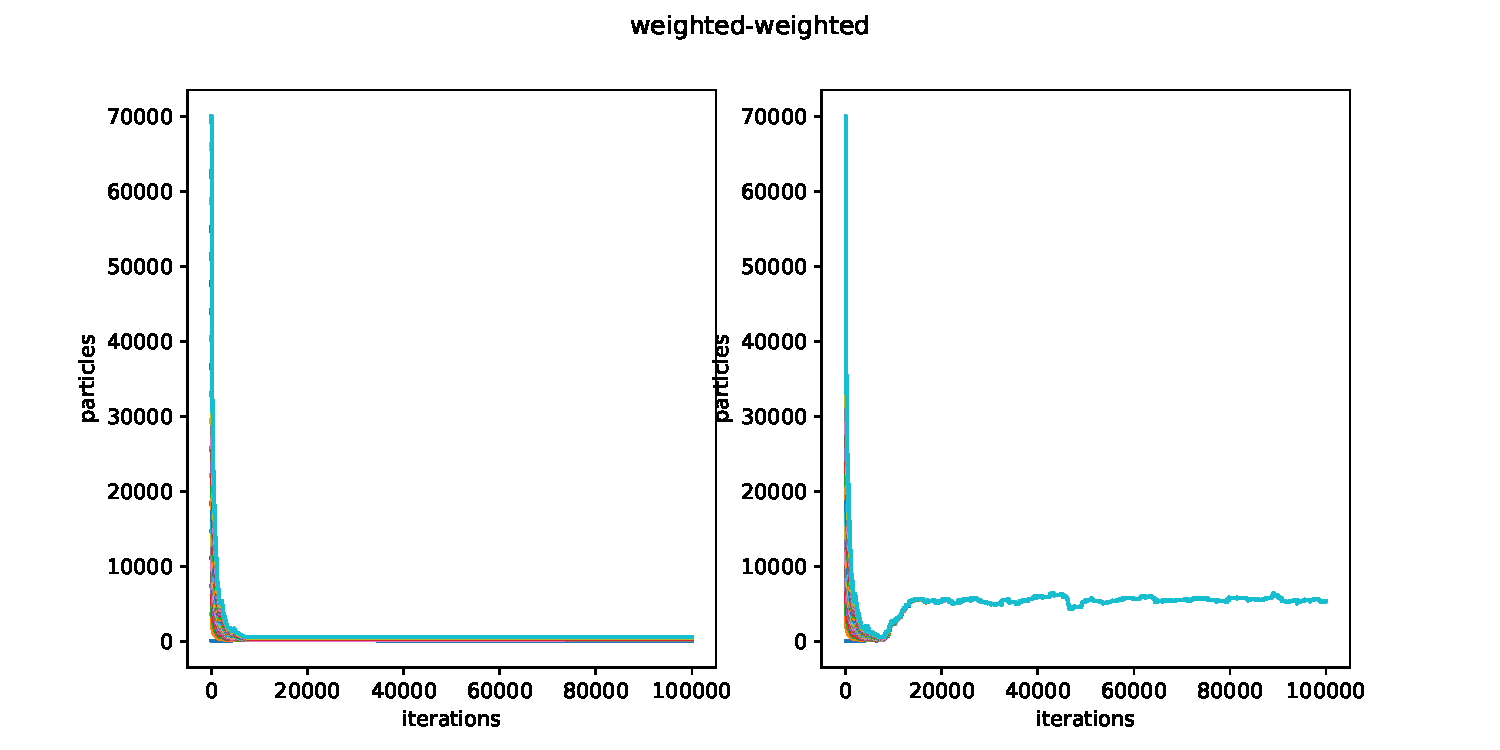
\includegraphics[width=\linewidth]{RiverSwim/particles_weighted-weighted.pdf}
  \label{fig:riverswim_particles_weighted_weighted}
  \caption{}
\end{subfigure}

\bigskip
\centering
\begin{subfigure}{\linewidth}
  \centering
  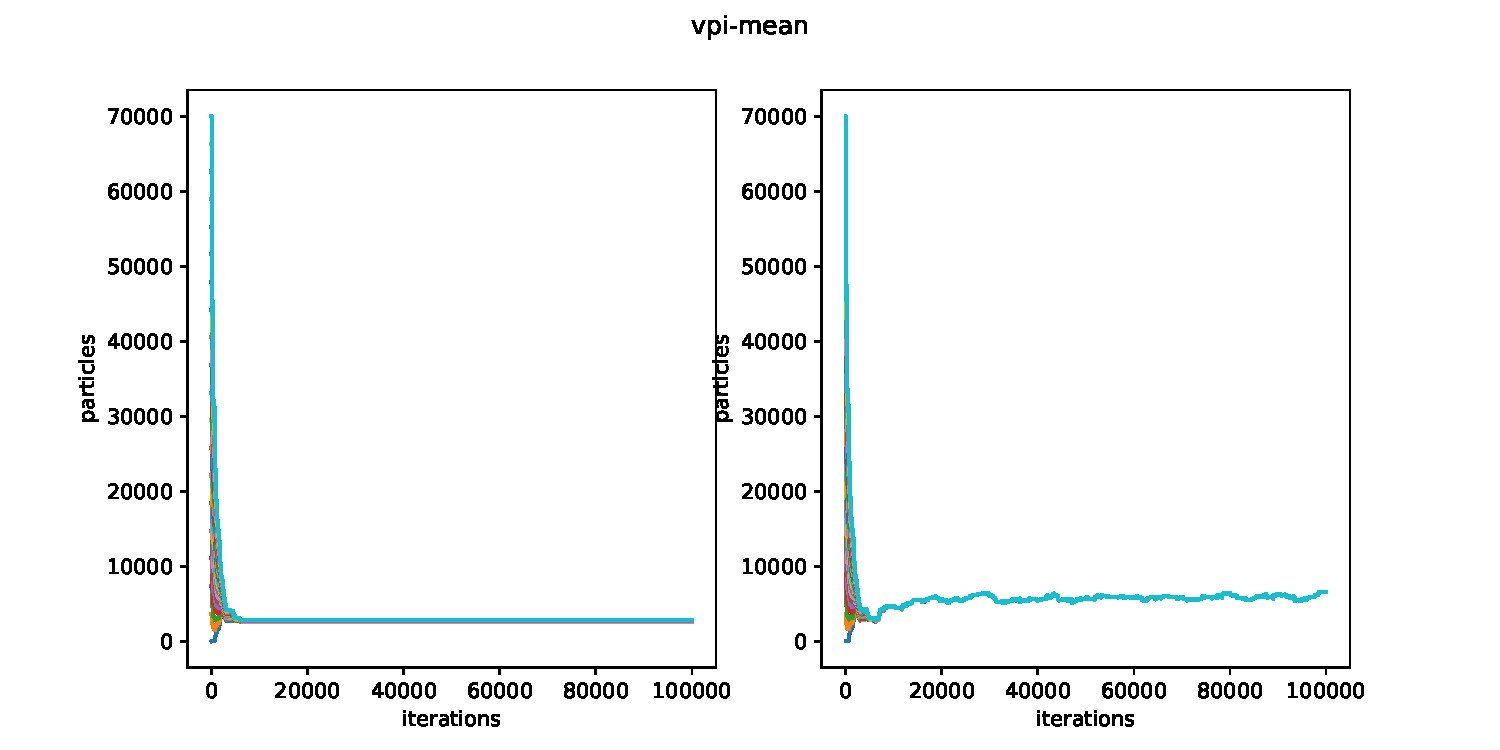
\includegraphics[width=\linewidth]{RiverSwim/particles_vpi-mean.pdf}
  \caption{}
  \label{fig:riverswim_particles_vpi_mean}
\end{subfigure}
\caption{Evolution of the particles in the first state of the RiverSwim domain during the learning process for the Particle Q-learning algorithm with weighted policy and weighted update (a), and VPI policy and maximum mean update (b). The optimal action is shown on the right, while the suboptimal action is shown on the left on both (a) and (b).}
\label{fig:riverswin_particle_evolution}
\end{figure}
Both Q-learning versions fail to learn the optimal policy. The other algorithms learn fairly quickly. PQL\_V\_M again is the fastest learner. While BQL starts better, is again surpassed in performance by PQL\_W\_W, which learns faster in this domain compared to the previous. This domain has two actions available in every state. Once again we will discuss the evolution of the particles of these two actions in the first state. Figure~\ref{fig:riverswim_particles_vpi_mean} shows how the particles evolve for the same versions of PQL we have investigated in the previous domains. What we can see here, is that the algorithms are robust \wrt the choice of the initialization interval. We can see that, even though the particles are initialized in a large interval, they quickly converge to the true Q-value. This can be seen also in Figure~\ref{fig:riverswim_std_evolution} where the standard deviation of the particles is shown to quickly converge to 0, for both algorithms, for both actions.\par
\begin{figure}
\centering
\begin{subfigure}{\linewidth}
  \centering
  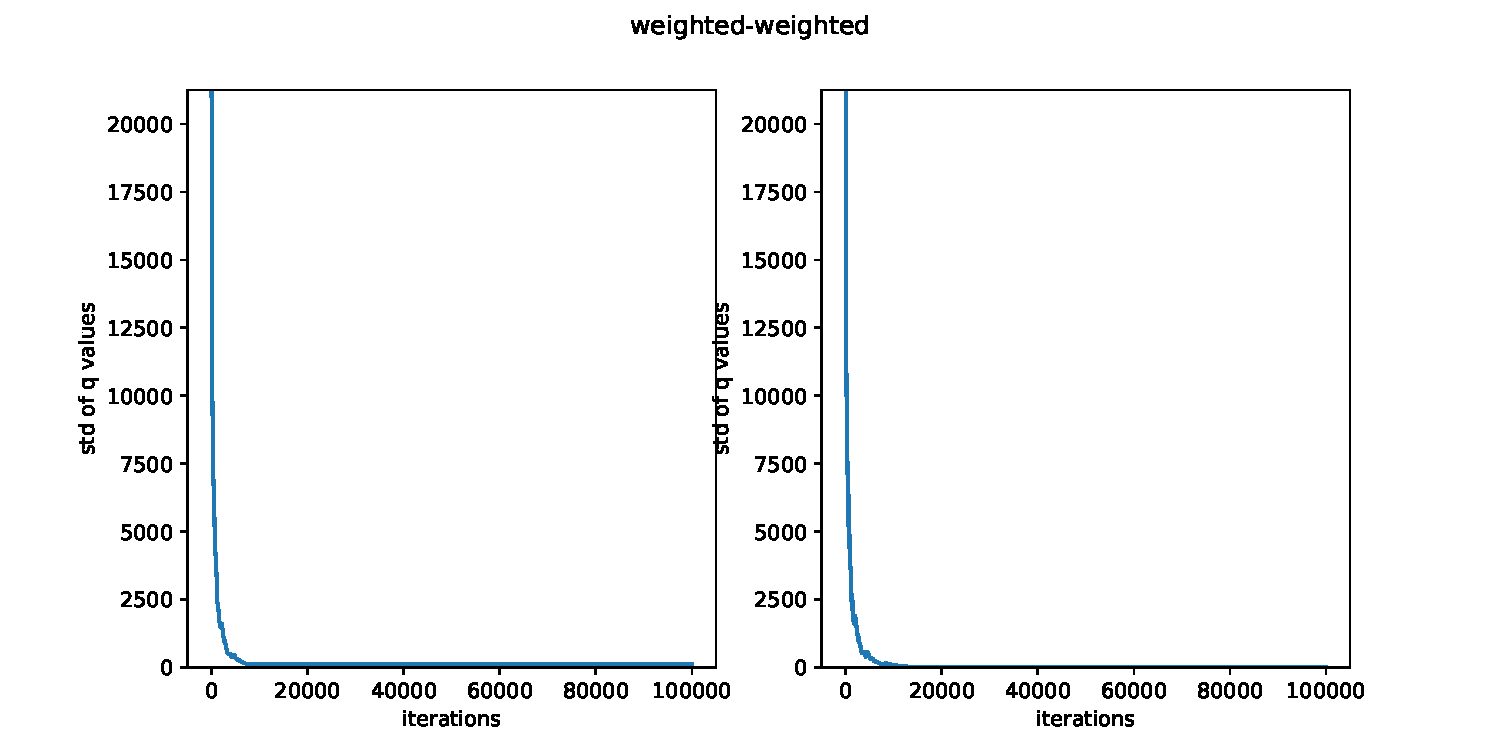
\includegraphics[width=\linewidth]{RiverSwim/std_weighted-weighted.pdf}
  \label{fig:riverswim_std_weighted_weighted}
  \caption{}
\end{subfigure}%

\bigskip
\centering
\begin{subfigure}{\linewidth}
  \centering
  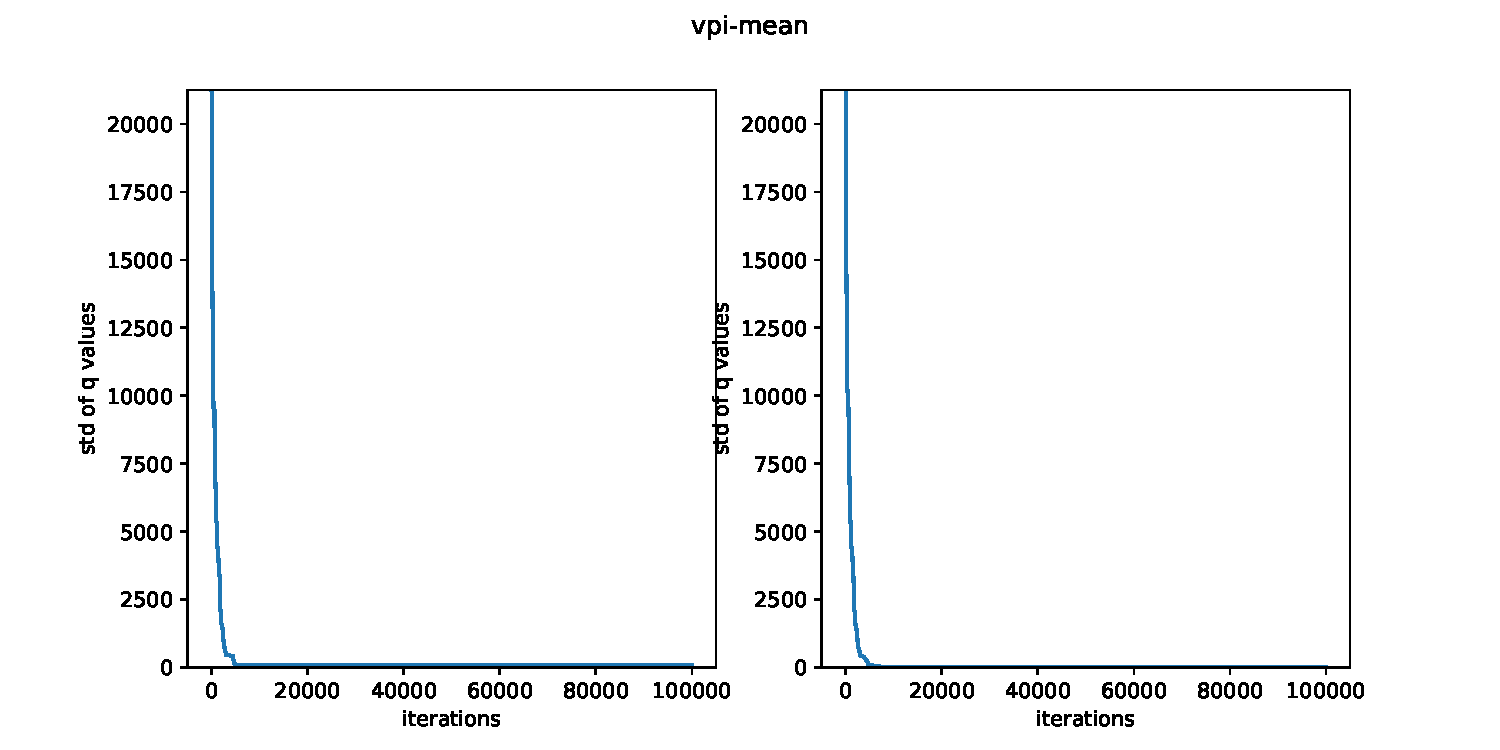
\includegraphics[width=\linewidth]{RiverSwim/std_vpi-mean.pdf}
  \label{fig:riverswim_std_vpi_mean}
  \caption{}
\end{subfigure}
\caption{Standard deviation of the particles as a function of the learning timestep for the Particle Q-learning algorithm with weighted policy and weighted update (a), and VPI policy and maximum mean update (b) in the RiverSwim domain. The optimal action  is shown on the right, while the suboptimal action is shown on the left on both (a) and (b).}
\label{fig:riverswim_std_evolution}
\end{figure}
Finally, we show, in Figure~\ref{fig:riverswim_prob_evolution}, the probability of exploration in the first state as a function of the learning step. Again, this probability converges to 0.
\begin{figure}
  \centering
  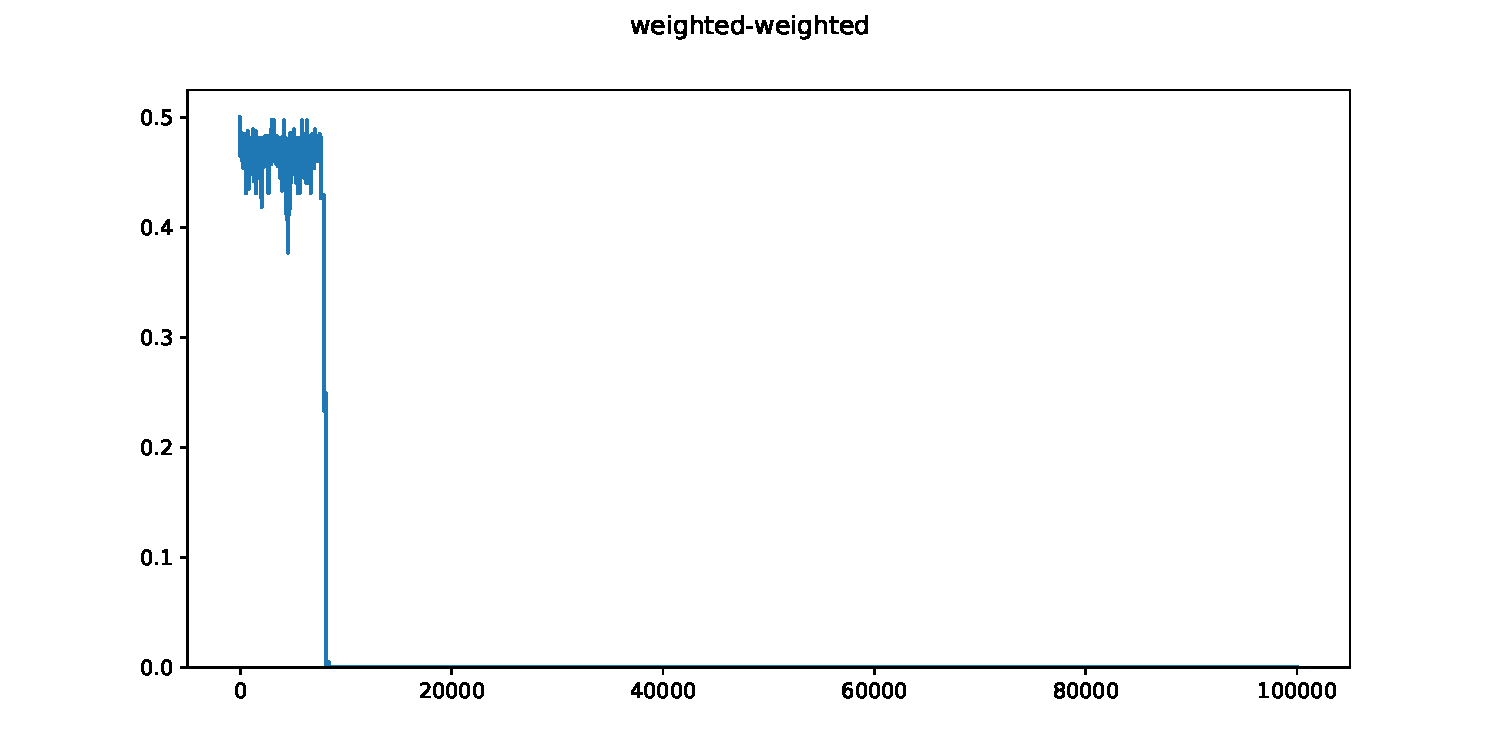
\includegraphics[width=\linewidth]{RiverSwim/prob_weighted-weighted.pdf}
  \label{fig:riverswim_prob_weighted_weighted}
\caption{Probability of exploration as a function of the learning timestep for the Particle Q-learning algorithm with weighted policy and weighted update in the RiverSwim domain.}
\label{fig:riverswim_prob_evolution}
\end{figure}
\subsection{Six Arms Domain}
The next environment is again taken from ~\cite{Strehl2008AnAO}. Six Arms, shown in Figure ~\ref{fig:sixarms_domain}, consists of seven states, one of which is the initial state. For how it is build, Six Arms resembles a multi armed bandit problem. The agent must choose from six different actions. Each action pulls a different arm, with a different payoff probability. When the arm pays off, the agent is sent to another state. Within that new state, large rewards can be obtained. The higher the payoff probability for an arm, the smaller the reward received (from the room the agent is sent to by the arm). In this MDP, a decision maker can make use of smaller amounts of experience on the low paying arms and still perform well.\par
\begin{figure}
 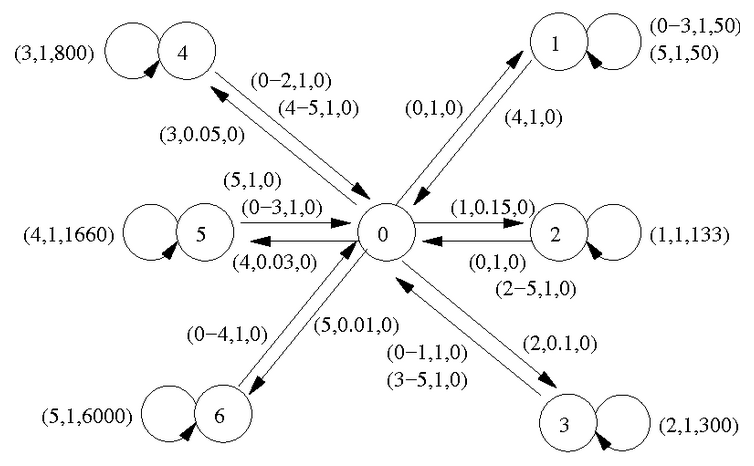
\includegraphics[width=\linewidth]{sixarms_domain.png}
 \caption{Six Arms domain taken from ~\cite{Strehl2008AnAO}.} ~
\label{fig:sixarms_domain}
\end{figure}
Figure~\ref{fig:sixarms_learning_curve} shows the results of our tests in the SixArms domain. Training episodes are the same as in River Swim, Chain and Loop domains. Once again PQL\_V\_M learns faster than the other algorithms. Simple exploration approaches (Boltzmann and $\epsilon$-greedy) fail to learn again. We note the fact that Particle Q-learning with VPI policy and weighted update (PQL\_V\_W) also perform extremely badly. Six Arms is a highly non deterministic domain, and exploration here is really important. VPI policy stops exploration rather quickly and fails to find the optimal actions. We saw this also in the previous domains. The algorithms converged quickly, but the domains were simpler, so VPI policy performed better. PQL\_W\_W on the other hand learns slower than PQL\_V\_M but still better than BQL approaches. BQL with weighted policy seems to have an advantage in the offline setting after the last periods of training, but the behaviour is rather unstable, also due to the uncertainty of the domain itself.
\begin{figure}
 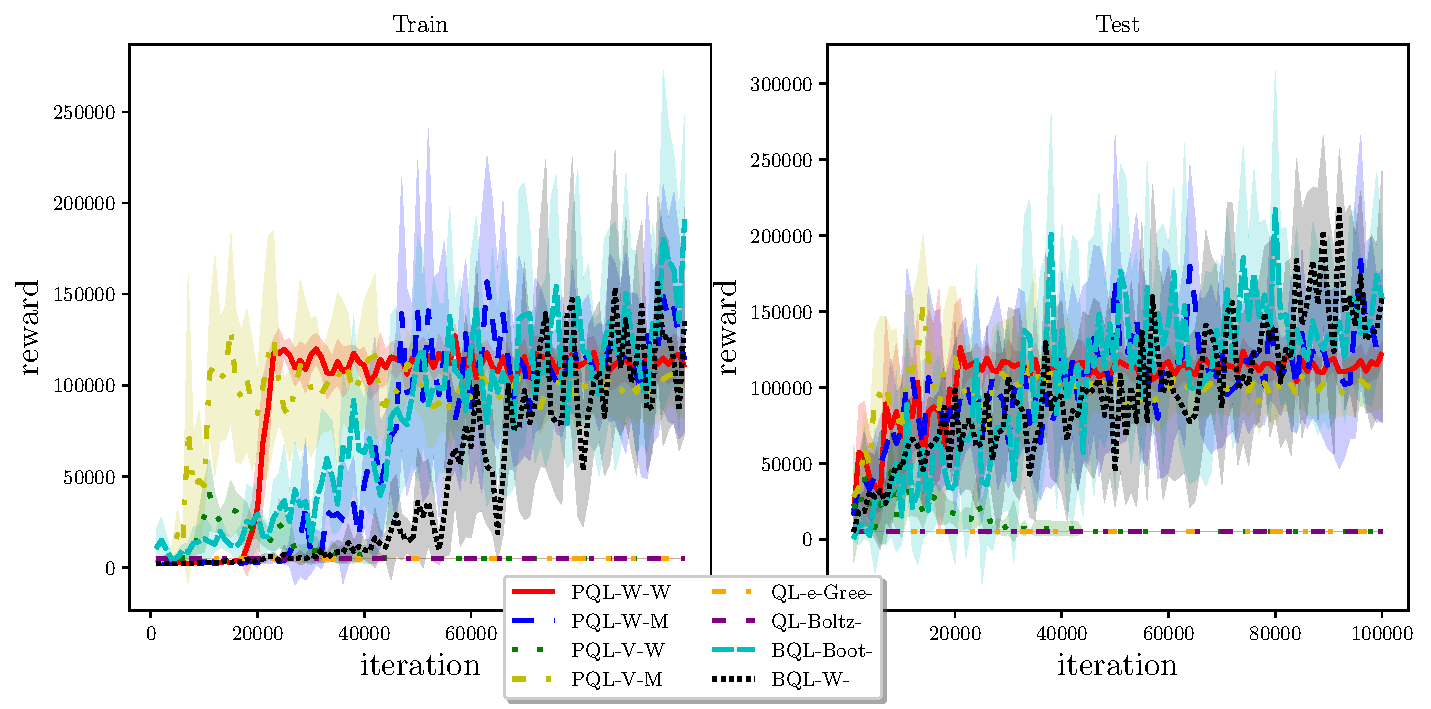
\includegraphics[width=\linewidth]{SixArms/learning_curve.pdf}
 \caption{Online and offline scores in the SixArms domain.}
 \label{fig:sixarms_learning_curve}
\end{figure}
\subsection{Knight Quest}
The last environment we will test our algorithm in is called Knight Quest~\cite{DBLP:conf/icml/FruitPLO18}. This environment takes inspiration from classical arcade games. The goal is to rescue a princess in the shortest time without being killed by the dragon. To achieve this task, the knight needs to collect gold, buy the magic key and reach the princess location. A representation of the game is given in Figure ~\ref{fig:knightquest_domain}.\par
\begin{figure}
 \centering 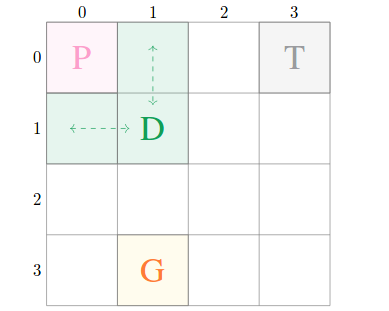
\includegraphics[width=10cm]{knightquest_domain.png}
 \caption{Knight Quest domain taken from ~\cite{DBLP:conf/icml/FruitPLO18}. The green cells are the three locations the dragon can move to.} ~
\label{fig:knightquest_domain}
\end{figure}
The elements of the game are:
\begin{itemize}
\item The knight,
\item the princess,
\item the dragon patrolling the princess,
\item a gold mine,
\item a town.
\end{itemize}
The knight is the only player of the game. He moves in the environment using the four cardinal actions (\ie right, down, left and up) plus an action to keep the current position (stay). Additionally, the knight can collect the gold (collect gold), buy a key (buy key) or buy an armour (buy armour).\par
The town (T) is the place where the knight can buy objects and where it is reset when he rescues the princess or he is killed by the dragon. Saving the princess (P) is the objective, while the gold mine (G) is the place where the knight can collect gold. The dragon (D) is the enemy and it is randomly moving around the princess's location. The dragon can kill the knight when they are at the same position and the knight does not have the armour. We denote as $d \in \{0,1,2\}$ the position of the dragon such that: $d = 0 := (0,1)$, $d= 1 := (1,0)$ and $d= 2 := (1,1)$. The transition probabilities of the dragon are:
\begin{equation*}
p_d(\cdot \vert 0)=[0.4,0,0.6]; \qquad p_d(\cdot \vert 1)=[0,0.4,0.6]; \qquad p_d(\cdot \vert 2)=[0.4,0.2,0.4]. 
\end{equation*}
\par
The state $s_t$ of the game is represented by the following elements:
\begin{itemize}
\item Knight position: coordinates of the grid, $(row,col), \quad row,col \in \{0,1,2,3\};$
\item Gold level: the amount of gold own by the knight, $g \in \{0,1\}$;
\item Dragon position: $d \in \{0,1,2\}$;
\item Object identifier: the object(s) owned by the knight, $o=\{0,1,2,3\}$ where 0 := nothing, 1 := key, 2 := armour and 3 :=key and armour.
\end{itemize}
The movement actions have the trivial effect of changing the knight position. The
action \emph{collect gold} changes the state only when the knight is at the mine. In this case the level of gold is incremented by one, formally $g_{t+1}= \min \{1,g_t + 1\}$. Actions \emph{buy key} and \emph{buy armour} alter the state only when are executed in the town with gold-level equal to 1. All the actions are deterministic when the knight does not own the armour. When the knight has the armour: 
\begin{itemize}
\item The movement actions result in a normal transition with probability 0.5, otherwise the current position is kept;
\item The \emph{collect gold} action fails with probability 0.9, \ie with probability 0.01 the gold level is increment by 1;
\item Actions \emph{buy key} and \emph{buy armour} are not modified.
\end{itemize}
When the knight is equipped with the armour it cannot be killed by the dragon (i.e., knight and dragon can occupy the same cell). At the same time, the armour makes the collection of the goal very challenging (i.e., success probability is 0.01).\par
The basic reward signal is $-1$ at each time step. Nevertheless, the knight receives a reward of $-10$ when he executes \emph{collect gold}, \emph{buy key} or \emph{buy armour} outside the designed location (i.e., mine and town).  The knight obtains a reward of $20$ when he reaches the princess with the key and $-20$ when he is killed by the dragon (i.e., knight and dragon are in the same cell and the knight
does not have the armour). Finally, when the episode ends (i.e., the knight reaches the princess with the key or he is killed), the knight is reset at town location with no gold or object ($g,o= 0$) and the dragon position is randomly drawn, $d \sim U(\{0,1,2\})$.\par
\begin{figure}
 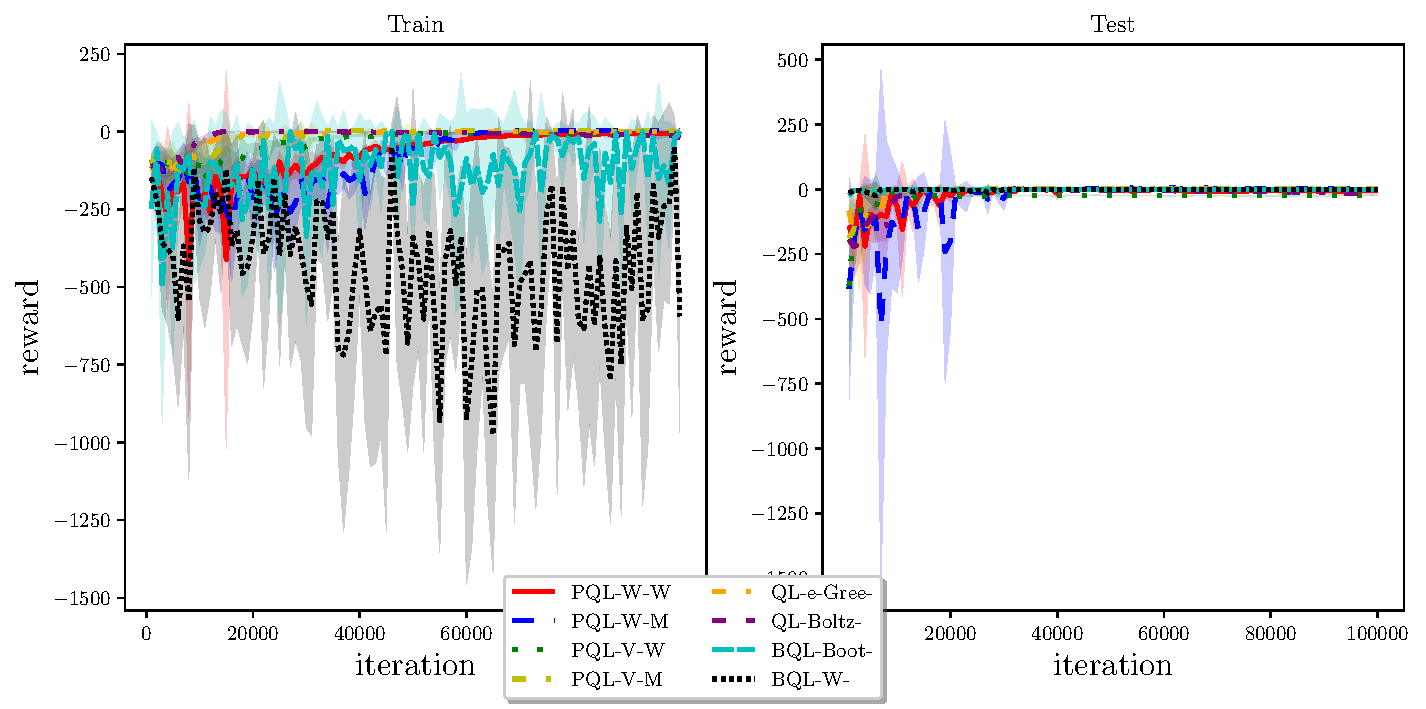
\includegraphics[width=\linewidth]{KnightQuest/learning_curve.pdf}
 \caption{Online and offline scores in the KnightQuest domain.}
 \label{fig:knightQuest_learning_curve}
\end{figure}
Figure~\ref{fig:knightQuest_learning_curve} shows the results of our tests in the KnightQuest domain with the same standard training periods. We can see that in the offline case, simple exploration strategies perform better. Q-learning with Boltzmann and $\epsilon$-greedy exploration quickly reach maximum reward (0 in this domain). Our PQL algorithms learn to achieve maximum rewards also, but slower since they perform exploration. It is interesting that BQL does not reach this maximum reward in the online case, for neither of the policy models. Nonetheless, in the offline evaluations, all algorithms achieve optimal performance rather quickly, with PQL\_W\_W being the slower algorithm. We think these results are due to the fact that this domain is a simple grid-world environment and does not require deep exploration.
\section{Atari Experiments}		 \label{sec:atari_experiments}
In this section we will discuss the results of the ``deep'' version of our algorithm, Particle DQN, and compare its results with Bootstrapped DQN. We chose to compare our results with Bootstrapped DQN because both algorithms perform deep exploration using Q-distributions. Indeed the architecture of the deep network we use to conduct the experiments was taken from ~\cite{DBLP:journals/corr/OsbandBPR16}, which in turn adapts the famous DQN architecture designed by Mnih et al. in ~\cite{mnih2015humanlevel}.\par
We test our algorithms using the Arcade Learning Environment (ALE) described in ~\cite{Bellemare:2013:ALE:2566972.2566979}. Although there is a large number of Atari games we could have tested the algorithms, we present here results obtained in two games, due to the long training time required by the algorithm. It takes three to four days to train the agents in a single Atari game, this by considering training periods only a quarter of the length of the standard of the literature. This is further worsened by the fact that we had to run multiple instances of each algorithm in each environment to show the mean performance over multiple runs (a standard in literature to account for the random initialization of the deep networks).
\subsection{Experimental Setup}
Again we are testing for deep exploration, but in this section we focus in Atari games. Each step of the agent corresponds to four steps of the emulator, where the same action is repeated. The reward values observed by the agents are clipped between -1 and 1 for stability. We evaluate our agents and report performance based upon the raw scores and not the discounted scores. As it is common in literature, we do not show the online performance of the agent during training. We show the scores collected, when exploiting the greedy policies derived from the Q-function after each training period.\par
The \emph{convolutional} part of the network used is identical to the one used in ~\cite{DBLP:journals/corr/OsbandBPR16}. The input to the network is $4\times 84 \times 84$ \emph{tensor} with a rescaled, grayscale version of the last four observations. The first convolutional layer has 32 filters of size 8 with a stride of 4. The second layer has 64 filters of size 4 with stride 2. The last layer has 64 filters of size 3. We split the network beyond the final layer into $N = 20$ distinct heads, each one is fully connected and identical to the network in ~\cite{DBLP:journals/corr/OsbandBPR16}. This consists of a fully connected layer to 512 units followed by another fully connected layer to the Q-Values for each action. The fully connected layers all use \emph{Rectified Linear Units} (ReLU) as a \emph{non-linearity}. We normalize gradients $\frac{1}{N}$ that flow from each head as in ~\cite{DBLP:journals/corr/OsbandBPR16}.
We trained the networks with \emph{RMSProp} optimizer. The discount was set to $\gamma = 0.99$, the number of steps between target updates was set to $\tau= 10000$ steps. We trained the agents for a total of 12.5M steps per game, which corresponds to 50M frames. The agents were evaluated every 1M frames. \par
The \emph{experience replay} contains the 1M most recent transitions. We update the network every 4 steps by randomly sampling a minibatch of 32 transitions from the replay buffer to use the exact same minibatch schedule as Bootstrapped DQN. \par
We show the results of our tests in 3 algorithms: Bootstrapped DQN (Boot\_DQN), Particle DQN with weighted policy and weighted update (P\_DQN\_W\_W), Particle DQN with weighted policy and maximum mean update (P\_DQN\_W\_M). The versions using VPI policy because they did not show good results in preliminary tests. As a result, for time considerations, we did not conduct the full tests on Particle DQN with VPI policy. All algorithms use 20 network heads, \ie we use 20 particles in Particle DQN and $K=20$ in Bootstrapped DQN. We used exactly the same network architecture for all algorithms.
\subsection{Breakout}
In this section we will discuss the experiments conducted on the Breakout Atari 2600 game. A frame from the game is shown in Figure~\ref{fig:breakout_frame}. In this game multiple layers of bricks are positioned in the top of the screen. A ball moves across the screen and bounces at the sides of the screen and at the bricks. When the ball bounces off a brick the brick is removed from the screen and the player gains points. If the ball reaches the bottom of the screen, the player loses a turn. To prevent this from happening the player can move a paddle situated at the bottom of the screen, to bounce the ball back up. The objective of the game is to remove bricks and collect scores as a result. The highest achievable score is 896.\par
We simulated the game through the ALE~\cite{Bellemare:2013:ALE:2566972.2566979}. In the simulator, the game has 4 possible actions. Figure~\ref{fig:breakout_learning_curve} shows the learning curves of the three algorithms considered. We can see that the algorithms have similar performance, with our Particle algorithms scoring slightly higher than Boot\_DQN. An interesting result is that our algorithms seem to be more stable than Boot\_DQN. Being that we implemented the deep networks for both algorithms with the same architecture, if the instability observed in Bootstrapped DQN was a result of the network, we would observe it in all algorithms. This suggests that Particle DQN improved the stability of the agent. 
\begin{figure}
 \centering 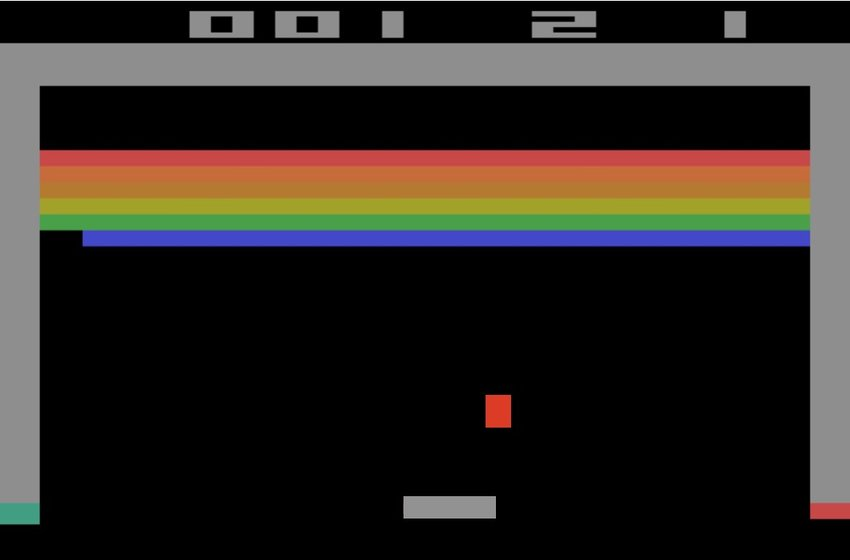
\includegraphics[width=0.7\linewidth]{breakout_frame.jpeg}
 \caption{Frame taken from the Breakout Atari 2600 game.}
 \label{fig:breakout_frame}
\end{figure}
\begin{figure}
 \centering 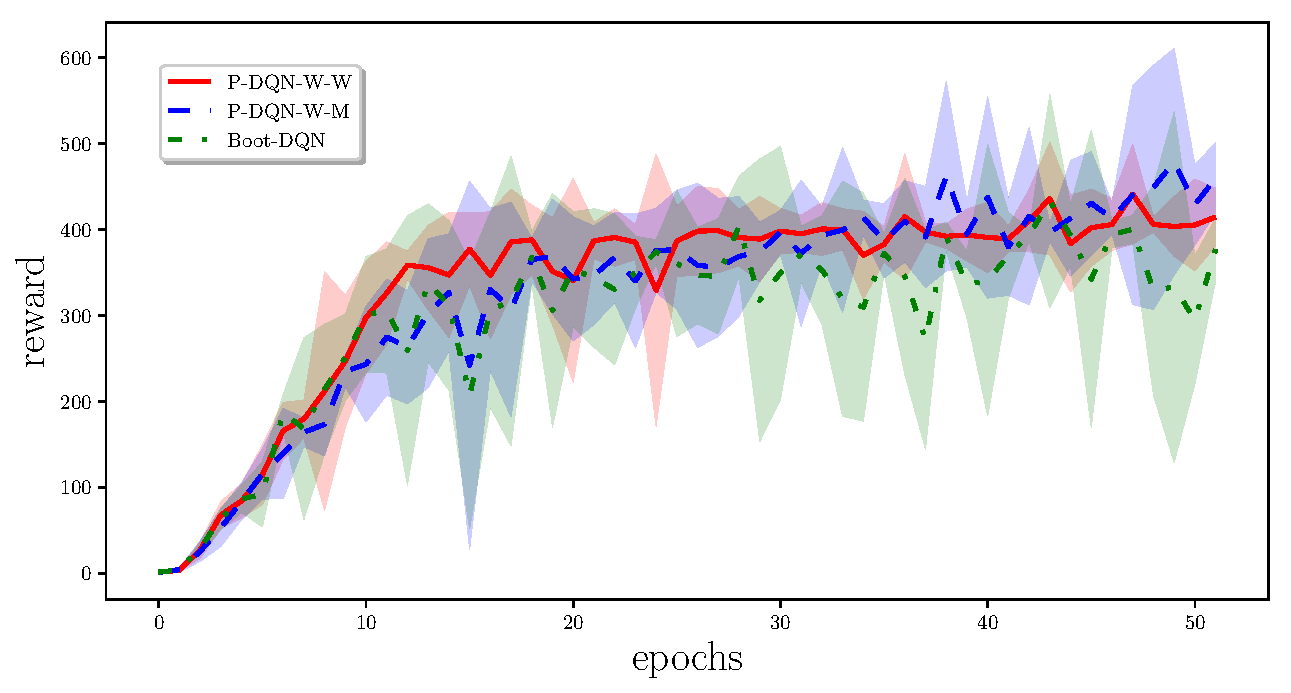
\includegraphics[width=\linewidth]{Breakout/learning_curve.pdf}
 \caption{Evaluation scores in the Breakout Atari 2600 game.}
 \label{fig:breakout_learning_curve}
\end{figure}
\subsection{Montezuma's Revenge}
Breakout is not a game that requires substantial exploration to be played. To test for deep exploration we tested the algorithms in Montezuma's Revenge, a famous Atari 2600 game. In this game, the player controls a character that moves in a 2D world. The character can move between rooms in a underground labyrinth. The objective is to score points by gathering jewels and killing enemies along the way. The agent must find keys to open doors, collect and use equipment such as torches, swords, amulets, etc., and avoid or defeat the challenges in his path.\par
\begin{figure}[H]
 \centering 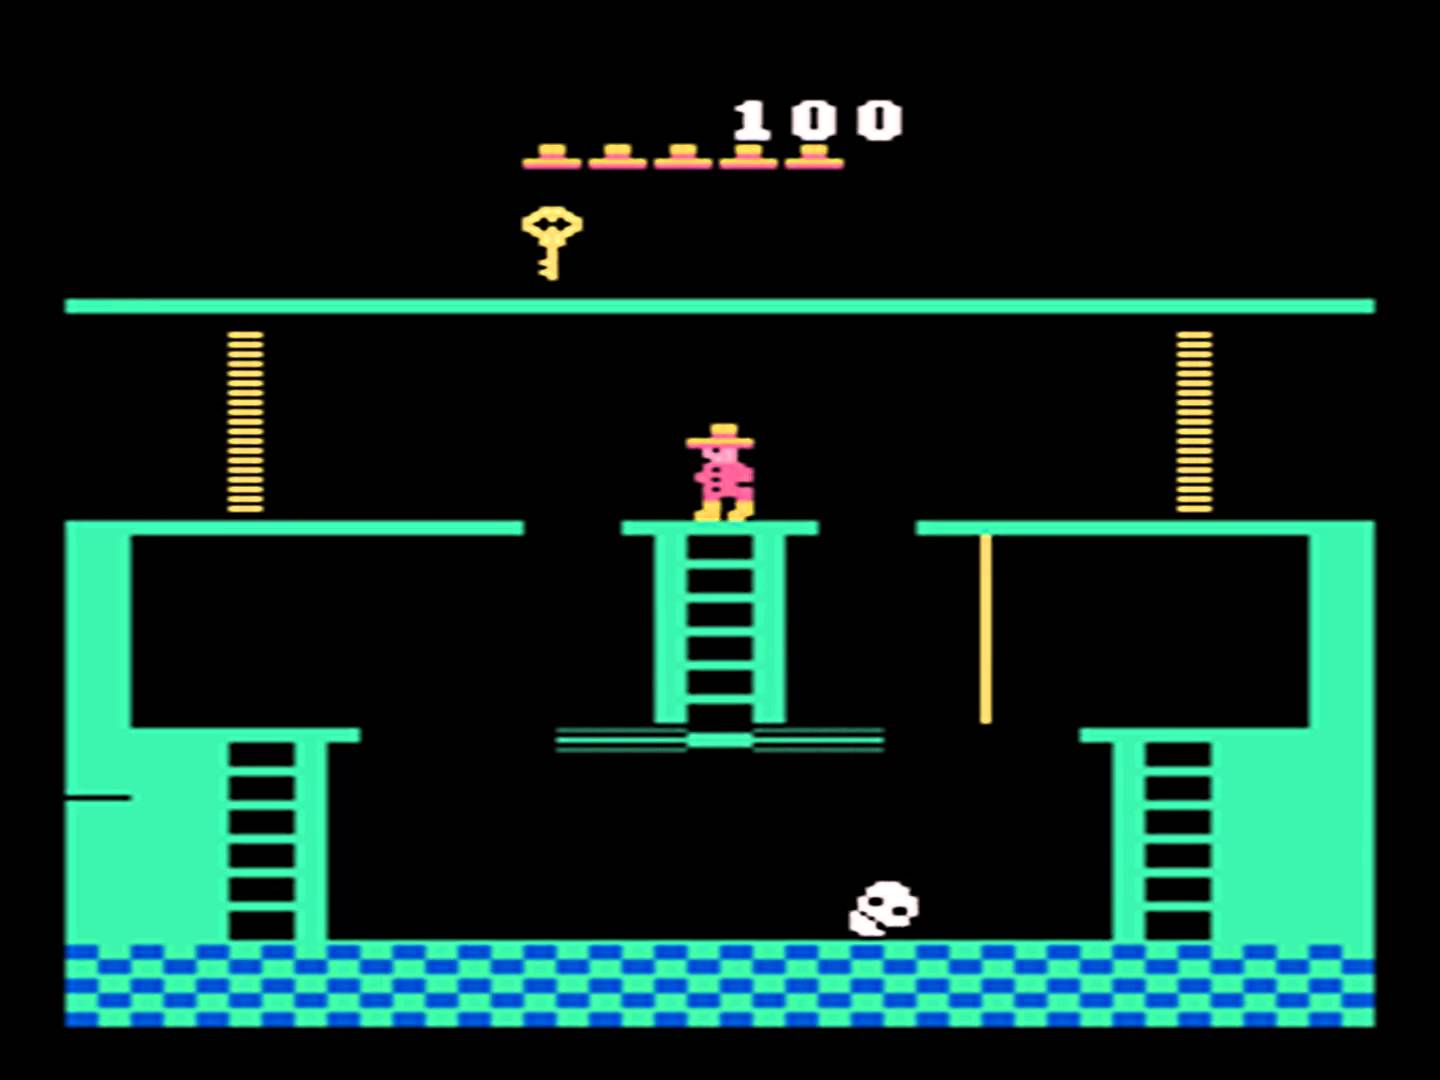
\includegraphics[width=0.7\linewidth]{montezuma_revenge_frame.jpg}
 \caption{Image of the first room of Montezuma's Revenge.}
 \label{fig:montezuma_frame}
\end{figure}
The main characteristic of this game is the scarcity of rewards. As an example, in the first room of the game shown in Figure~\ref{fig:montezuma_frame} the player collects a reward of 100 points when it collects the key, and then another reward of 300 when it opens one of the doors. Reaching the key is extremely difficult, as the agent will die if he falls from a hight or if he touches the enemy (white skull). To move in the following room, the agent needs to follow a very specific route to the key and back to the door. Exploration is extremely important in this domain because the agent requires long sequences of very specific actions to experience any reward, and such sequences are extremely unlikely to occur randomly. As a result, this is considered as one of the most difficult games to beat in the deep RL literature.\par
Figure~\ref{fig:montezuma_learning_curve} shows the results of testing the algorithms in Montezuma's Revenge. Indeed the game lives up to its reputation. Boot\_DQN and P\_DQN\_W\_W fail to score any points in this game. On the other hand, P\_DQN\_W\_M, in all the independent runs, manages to pass to the second room of the game and score 400 points in the process. Unfortunately, the agent does not learn to exploit this in future games. As a result, we see some spikes in the learning curve but no stable growth.
\begin{figure}[H]
 \centering 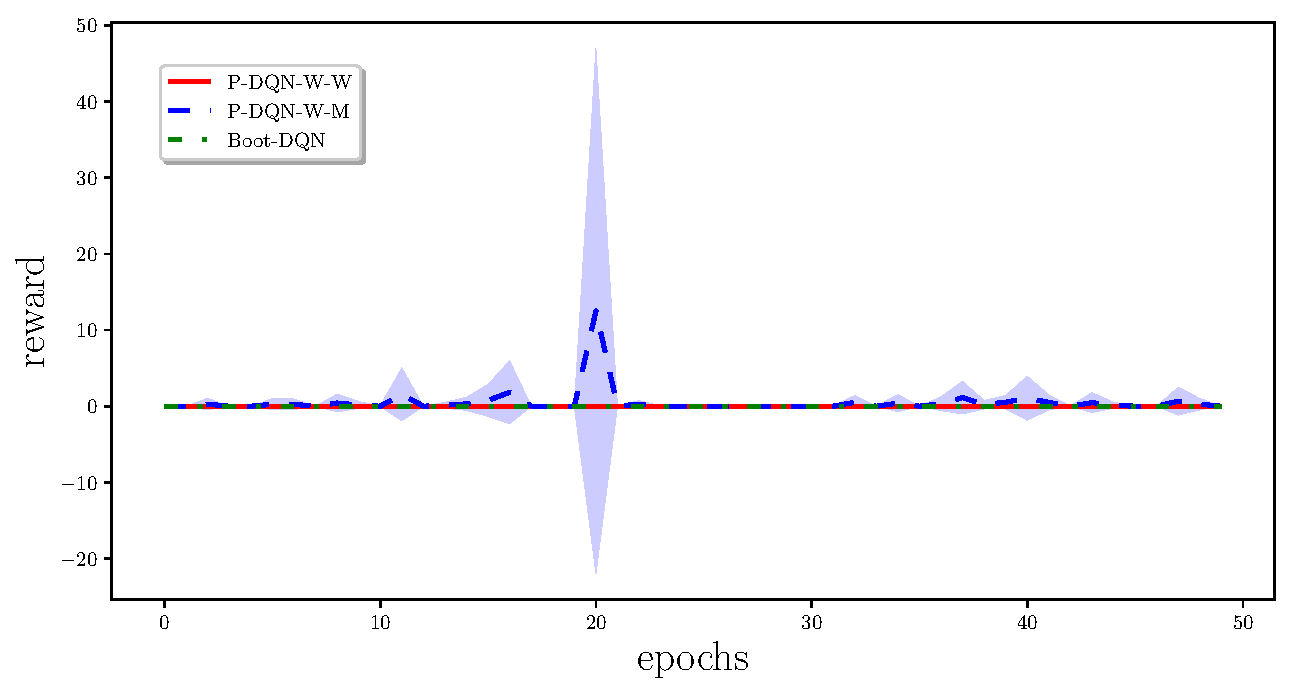
\includegraphics[width=\linewidth]{Montezuma/learning_curve.pdf}
 \caption{Evaluation scores in Montezuma's Revenge.}
 \label{fig:montezuma_learning_curve}
\end{figure} 
\chapter{Conclusions}		\label{chap:chapter6}
In this thesis we addressed the exploration vs. exploitation dilemma and proposed a new model-free algorithm that performs deep exploration by estimating the uncertainty about the agent's Q-values. We argued about the importance of maintaining Q-distributions to estimate this uncertainty, and further use these Q-distributions to drive exploration. We derived some interesting results on approximating the Q-distributions using the mixture of deltas model. We call these distributions Particle Q-Distributions. We compared our algorithm with some classical approaches to exploration as well as with Bootstrapped Q-learning, a state of the art algorithm that uses a similar approach to ours to drive exploration. We tested on various domains, some designed to encourage exploration as well as some simple navigation problems. Our algorithm showed improvements, sometimes substantial, in learning speed compared to Q-learning and Bootstrapped Q-learning when tested in finite MDPs. In the Taxi domain, not only we learned faster, but we also found the optimal policy of picking-up all the passengers, which Q-learning and Bootstrapped Q-learning failed to do.\par
We observed how the Q-distribution ``shrinked'' as the agent gathered more observations, driving the uncertainty about the agent's Q-values to zero. When using the weighted policy, this brought the probability of exploration to zero, and the agent exploits its current Q-values. Differently from classic exploration approaches, like $\epsilon$-greedy, we do not need to explicitly define a schedule of exploration that vanishes as the state-action counters increase. Our agent will stop exploration automatically when it is certain about its Q-value estimates.\par
A drawback of our algorithm is the increased spatial and computational complexity. Compared to classical Q-learning, we now need to store $M$ times more values, as we will store the Q-distributions instead of the Q-values. On the other hand, we have the same spatial complexity as Bootstrapped Q-learning. However, our algorithms come with a higher computational cost. Bootstrapped Q-learning does not have any substantial additional cost compared to classical Q-learning as it uses one Q-value estimate at a time (in the basic version). Our method, on the other hand, uses all estimates at any time to perform the updates, which gives us a linear complexity \wrt the number of particles (given that we do not sort the particles at every update). Additionally, we add the cost of the policies, which calculate the VPI or probability of being maximum at every timestep. This adds a substantial computational cost to our algorithms which we have not analyzed. Intuitively, this larger computational requirement is compensated by the faster convergence to the optimal policy.\par 
We extended the algorithm to the deep RL world by borrowing the architecture used  in Bootstrapped DQN. We tested two versions of the particle algorithms and Bootstrapped DQN in Atari 2600 games. We tried to initialize the networks in such a way that the output of the network represents the equally spaced particles in the interval $[q_{min},q_{max}]$ (same prior distribution we used in the tabular case). We did this by forcing this values in the last layer by inducing a bias. This unfortunately caused our agents not to be unstable and fail to learn as a result. Consequently, we decided to use the initialization of Bootstrapped DQN, \ie we initialized each head randomly.\par 
In Breakout we scored slightly better than Boot\_DQN and also improved the stability of the agent. The tests in Montezuma's Revenge showed some promising results but more work needs to be done. 
\subsubsection{Future Work}
We received some encouraging results about the learning speed of our particle algorithm. Despite these good experimental results, unfortunately we have not yet proved the ``efficiency'' of Particle Q-learning, \ie we do not have any bounds on the sample complexity or  regret. Something we leave for future work definitely is deriving these bounds. Moreover we have not done any analysis of the computational complexity of our particle algorithm. Computing the probabilities of each action to be maximal (in weighted policy or weighted update) comes with a high computational cost. We could approximate these probabilities by sampling but that would come with performance cost. We might try to balance these computational and performance costs. Finally, we leave to future work finding better ways to initialize the deep network when using our particle algorithm. Currently we initialize the network randomly. We might try to pre-train the network to initialize the heads in the desired interval. Furthermore, we did not do an analysis of the hyperparameters of the deep network. More work can be done in this aspect to improve learning speed and stability of the agent.  
\bibliographystyle{plain}
\bibliography{sample}
\appendix
\chapter{Experiments With Double Agents}
In this appendix we report the results of testing Particle Q-learning using the Double version of the algorithm, inspired from \cite{Hasselt:2016:DRL:3016100.3016191}. We tested the algorithms in the same domains described in Chapter \ref{chap:chapter5}, using the same experimental settings. Our PQL agents seem to be more unstable when used in their double version.
\subsubsection{Chain}
\begin{figure}[H]
 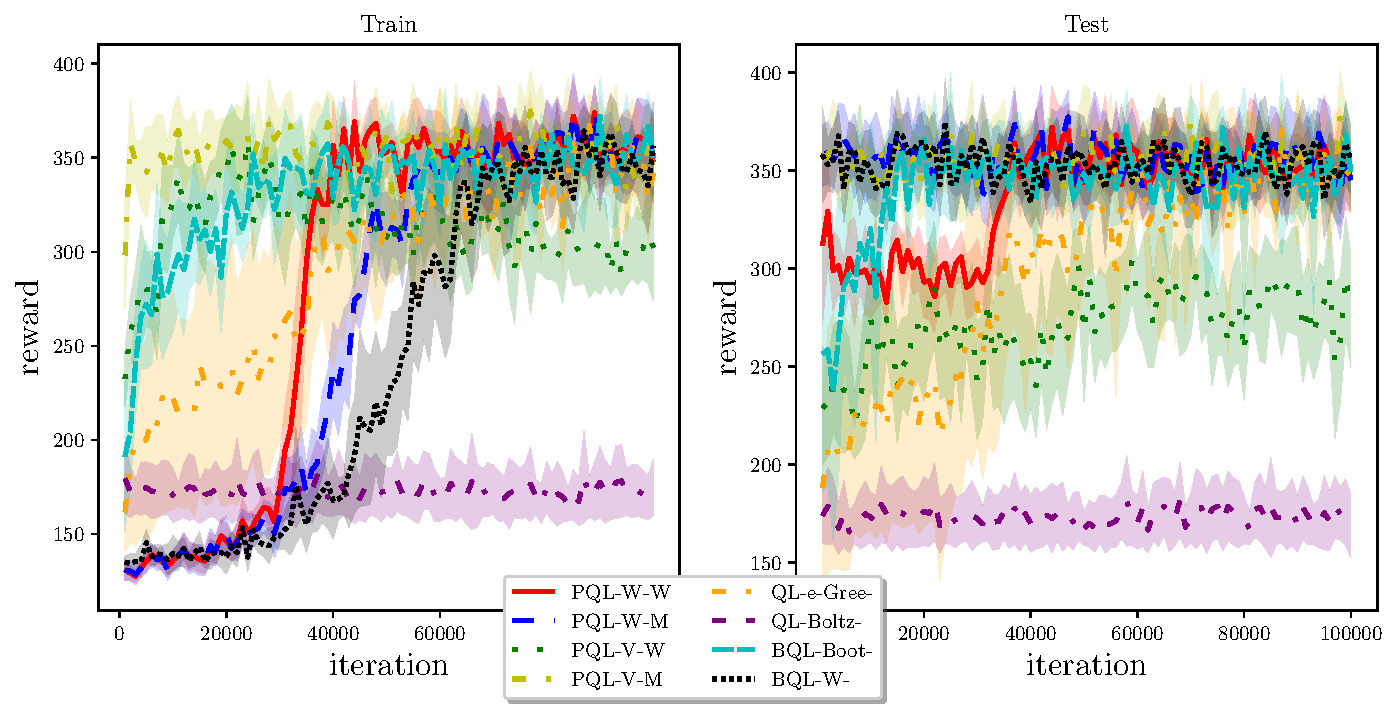
\includegraphics[width=\linewidth]{Chain/double_learning_curve.pdf}
 \caption{Online (left) and offline (right) scores for the double algorithms in the Chain domain.}
\end{figure}
\subsubsection{Loop}
\begin{figure}[H]
 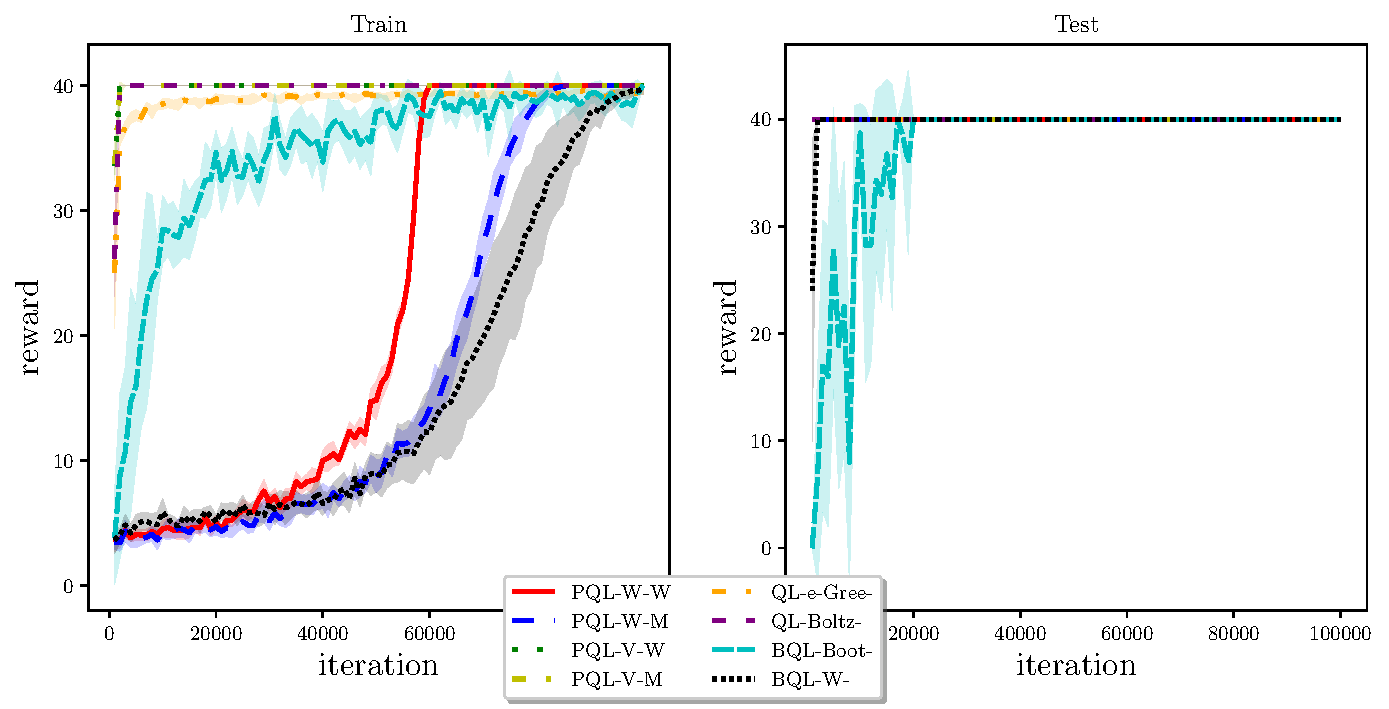
\includegraphics[width=\linewidth]{Loop/double_learning_curve.pdf}
 \caption{Online (left) and offline (right) scores for the double algorithms in the Loop domain.}
\end{figure}
\subsubsection{Taxi}
\begin{figure}[H]
 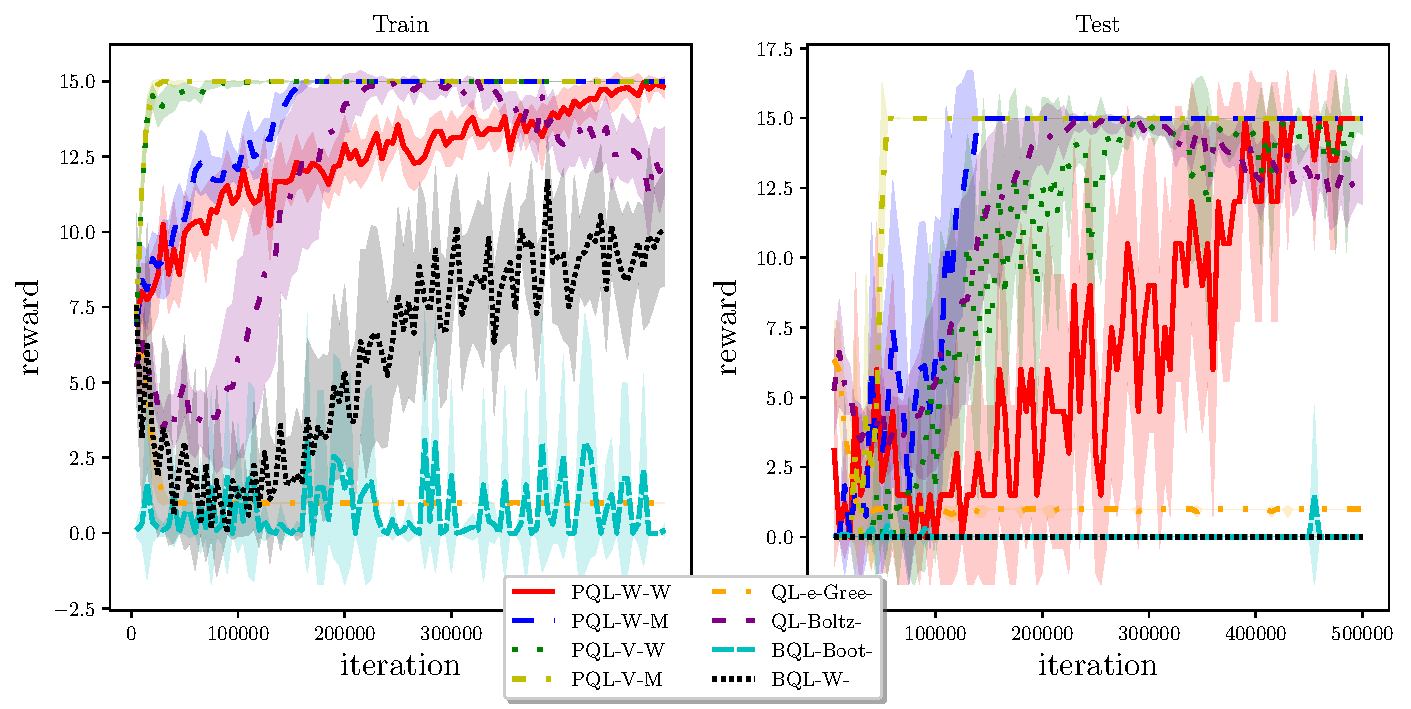
\includegraphics[width=\linewidth]{Taxi/double_learning_curve.pdf}
 \caption{Online (left) and offline (right) scores for the double algorithms in the Taxi domain.}
\end{figure}
\subsubsection{River Swim}
\begin{figure}[H]
 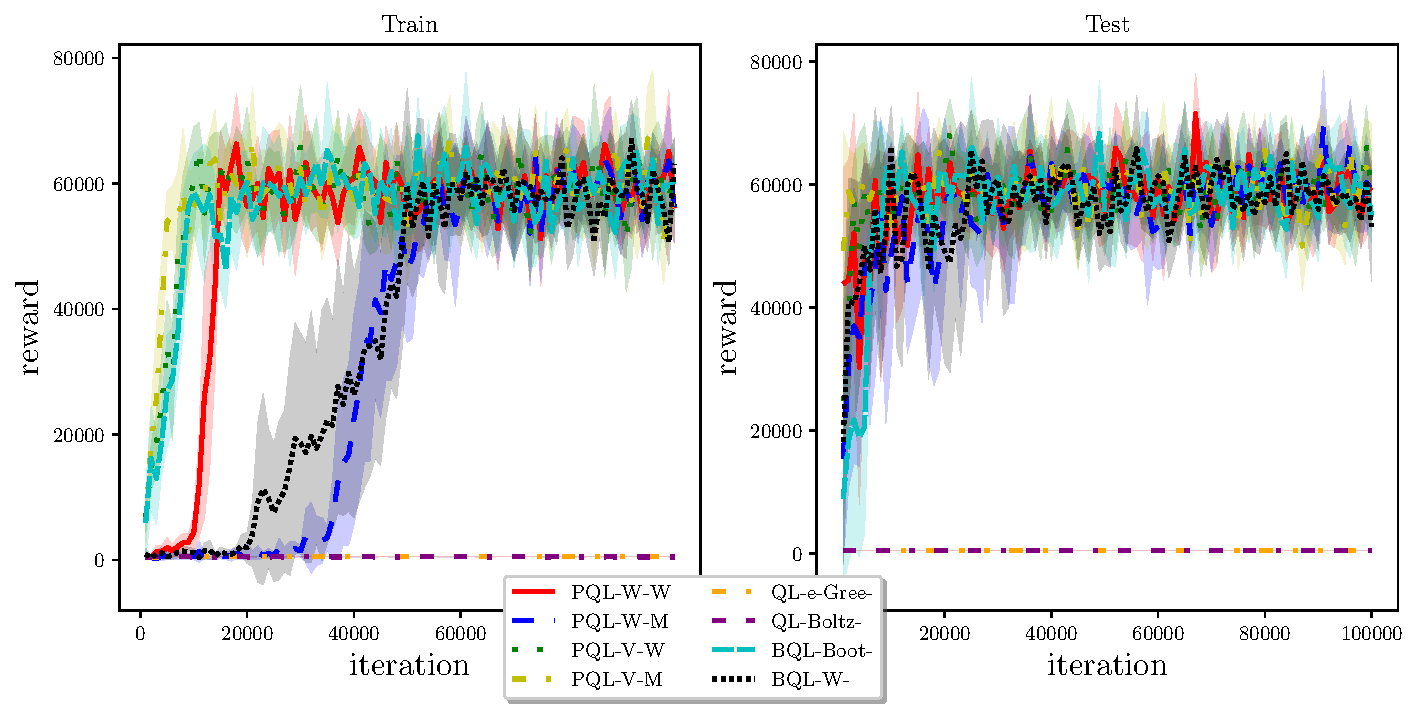
\includegraphics[width=\linewidth]{RiverSwim/double_learning_curve.pdf}
 \caption{Online (left) and offline (right) scores for the double algorithms in the River Swim domain.}
\end{figure}
\subsubsection{Six Arms}
\begin{figure}[H]
 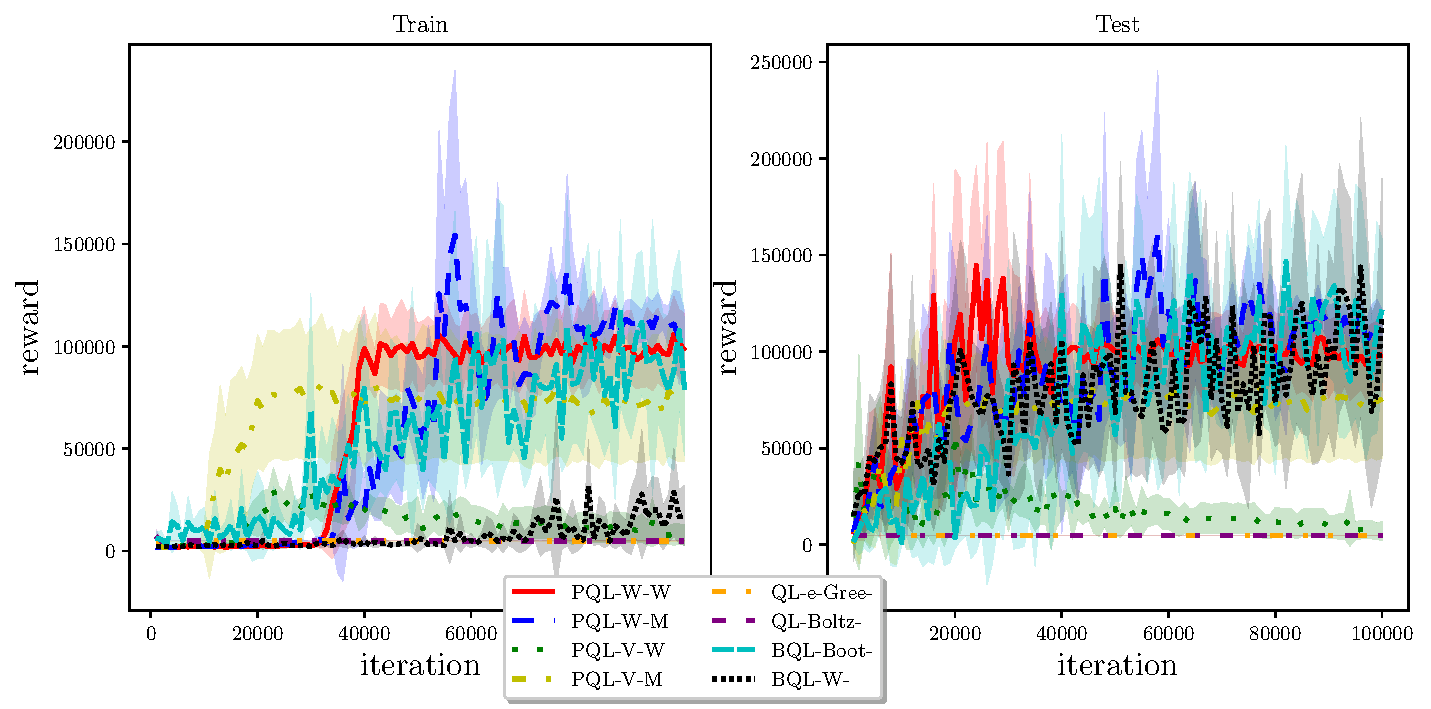
\includegraphics[width=\linewidth]{SixArms/double_learning_curve.pdf}
 \caption{Online (left) and offline (right) scores for the double algorithms in the Six Arms domain.}
\end{figure}
\subsubsection{Knight Quest}
\begin{figure}[H]
 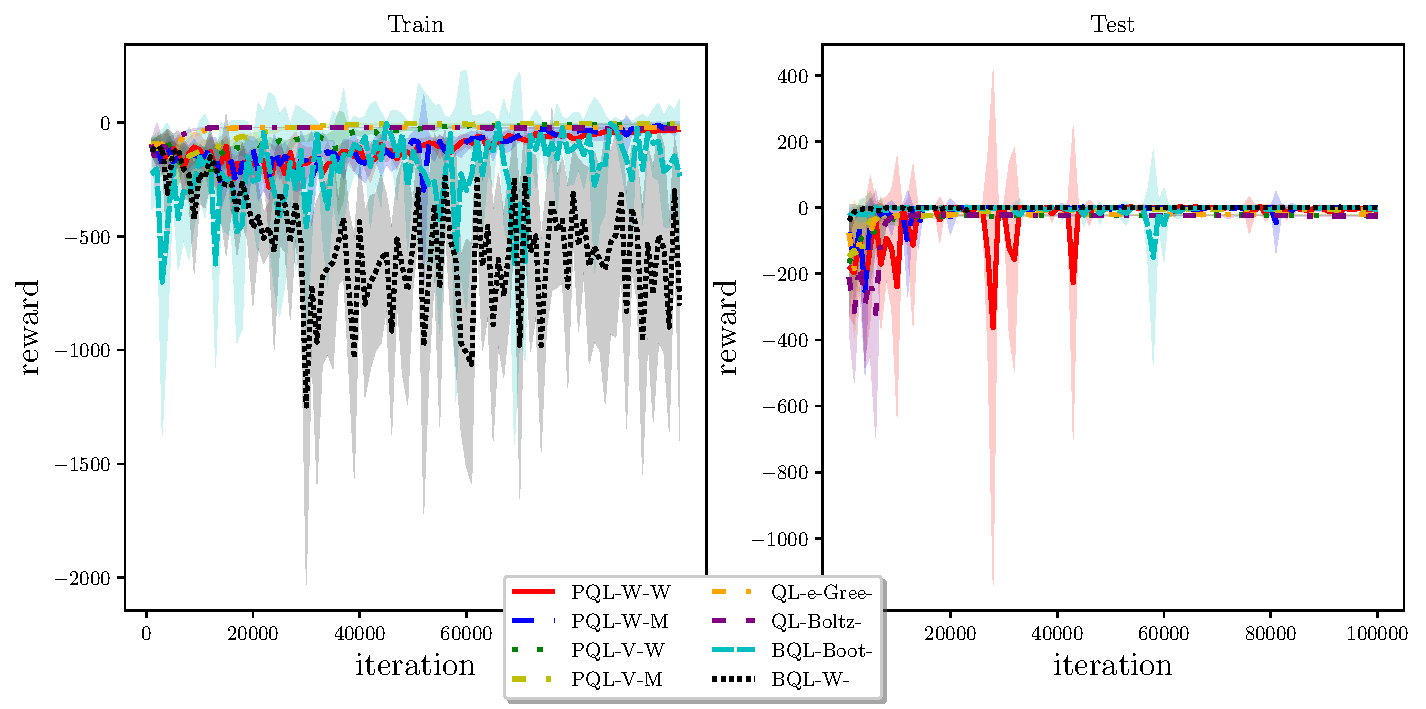
\includegraphics[width=\linewidth]{KnightQuest/double_learning_curve.pdf}
 \caption{Online (left) and offline (right) scores for the double algorithms in the Knight Quest domain.}
\end{figure}\label{app:appendixA}
\end{document}